\documentclass[11pt,twoside]{report}

 \pagestyle{headings}

\textwidth=440pt
\hoffset=-0.6truein

\usepackage{amsmath}
\usepackage{amsfonts}
\usepackage{amssymb}
\usepackage{dsfont}
\usepackage{pifont}
%\usepackage{bbold}
\usepackage{graphicx}
\usepackage{epstopdf}
\usepackage{epsfig}
%\usepackage{bibunits}
%\usepackage{theorem}
\usepackage[framed]{ntheorem}
\usepackage{framed}
%\usepackage{showlabels}
\usepackage{makeidx}
\usepackage{simplewick}
\usepackage{tikz-feynman}

\tikzfeynmanset{compat=1.0.0}  

\newcommand{\tick}{\ding{52}}
\newcommand{\notick}{\ding{56}}
\newcommand{\D}{\displaystyle}
\renewcommand{\chaptername}{Lecture}

\def\bfx{{\mathbf x}}
\def\bfxp{{\mathbf x^\prime}}
\def\bfy{{\mathbf y}}
\def\bfyp{{\mathbf y^\prime}}
\def\bfp{{\mathbf p}}
\def\bfpp{{\mathbf p^\prime}}
\def\ddt{\frac{d}{dt}}
\def\ddtt{\frac{d^2}{dt^2}}
\def\ie{{\it i.e.}\ }
\def\eg{{\it e.g.}\ }
\def\viz{{\it viz.}\ }
\def\matF{\mathcal F}
\def\matE{\mathcal E}
\def\GL{\mathrm{GL}}
\def\kpsi{|\psi\rangle}
\def\kpsione{|\psi_1\rangle}
\def\kpsitwo{|\psi_2\rangle}
\def\kpsionep{|\psi_1^\prime\rangle}
\def\kpsitwop{|\psi_2^\prime\rangle}
\def\kpsii{|\psi_i\rangle}
\def\kpsin{|\psi_n\rangle}
\def\kpsip{|\psi^\prime\rangle}
\def\bpsi{\langle\psi |}
\def\bpsione{\langle\psi_1 |}
\def\bpsitwo{\langle\psi_2 |}
\def\bpsii{\langle\psi_i |}
\def\bpsip{\langle\psi^\prime |}
\def\kphi{|\phi\rangle}
\def\kphione{|\phi_1\rangle}
\def\kphitwo{|\phi_2\rangle}
\def\kphii{|\phi_i\rangle}
\def\kphip{|\phi^\prime\rangle}
\def\bphi{\langle\phi |}
\def\bphione{\langle\phi_1 |}
\def\bphitwo{\langle\phi_2 |}
\def\bphii{\langle\phi_i |}
\def\bphip{\langle\phi^\prime |}
\def\bchi{\langle\chi |}
\def\bchione{\langle\chi_1 |}
\def\bchitwo{\langle\chi_2 |}
\def\bchii{\langle\chi_i |}
\def\bchip{\langle\chi^\prime |}
\def\kjm{|j,m\rangle}
\def\tr{\mathrm{Tr}}
\def\id{\mathds{1}}
{\theoremstyle{plain} \theorembodyfont{\rmfamily} \newframedtheorem{Ex}{Exercise}[section]}
{\theoremstyle{plain} \theorembodyfont{\rmfamily} \newtheorem{Def}{Definition}[section]}
{\theoremstyle{plain} \theorembodyfont{\rmfamily} \newtheorem{Thm}{Theorem}[section]}

\newcommand{\clearemptydoublepage}{\newpage{\pagestyle{empty}\cleardoublepage}}
\newcommand{\HRule}{\rule{\linewidth}{0.5mm}}
\newcommand{\iu}{\underline{i}}
\newcommand{\ju}{\underline{j}}
\newcommand{\ku}{\underline{k}}
\newcommand{\ru}{\underline{r}}
\newcommand{\pu}{\underline{p}}
\newcommand{\Lu}{\underline{L}}
\newcommand{\Ju}{\underline{J}}
\newcommand{\lap}{\nabla^2}
\newcommand{\ad}{\hat{a}}
\newcommand{\ac}{\hat{a}^\dagger}
\newcommand{\re}{\mathrm{Re}}
\newcommand{\ket}[1]{| #1 \rangle}
\newcommand{\bra}[1]{\langle #1 |}
\newcommand{\braket}[2]{\langle #1 | #2 \rangle}
\newcommand{\pref}[1]{(\ref{#1})}
\newcommand{\Eqref}[1]{Eq.~(\ref{#1})}
\newcommand{\del}{\v{\nabla}}				% Underlined del



\makeindex

\begin{document}

\title{Quantum Field Theory}
\author{L. Del Debbio, University of Edinburgh \\
  Version 0.1}

\pagenumbering{roman}
\maketitle
\clearemptydoublepage
\tableofcontents
\clearemptydoublepage

\pagenumbering{arabic}

\chapter{Introductory Thoughts}
\label{chap:intro}
\include{Sections/intro}

\chapter{Gaussian Integrals}
\label{chap:lec0}
\section{Multidimensional Gaussian Integrals}
\label{sec:mult-gauss-integr}

Consider the $n$-dimensional integral
\begin{equation}
  \label{eq:GaussIntOne}
  Z_A = \int d^nx\, \exp\left(
    -\frac12 \sum_{i,j=1}^n x_i A_{ij} x_j
    \right)\, .
\end{equation}
If $A$ is a complex, symmetric $n\times n$ matrix such that
\begin{align}
  & \re\ A \geq 0 \, ,\\
  & a_i \neq 0\, , \quad a_i\ \text{e.vals of }\ A\, ,
\end{align}
then 
\begin{equation}
  \label{eq:GaussIntTwo}
  Z_A = \left(2\pi\right)^{n/2} \left(\det A \right)^{-1/2}\, .
\end{equation}

\paragraph{General Gaussian Integral}

\begin{align}
  Z_A(b) &= \int d^nx\, \exp\left(
  -\frac12 \sum_{i,j=1}^n x_i A_{ij} x_j
  + \sum_{i=1}^n b_i x_i
  \right) \\
  \label{eq:GaussIntThree}
  &=  \left(2\pi\right)^{n/2} \left(\det A \right)^{-1/2}
    \exp\left(
  \frac12 \sum_{i,j=1}^n b_i \Delta_{ij} b_j
  \right) \, ,
\end{align}
where $\Delta = A^{-1}$. The existence of $\Delta$ is guaranteed by the non-vanishing e.vals of $A$.
\begin{Ex}
  Check the result in Eq.~\ref{eq:GaussIntThree} by changing the integration variables in the integral:
  \[
    x_i = y_i + \sum_{j=1}^n \Delta_{ij} b_j\, .
  \]
\end{Ex}

\section{Generating function}
\label{sec:generating-function}

Let $\mu$ be a measure in $\mathbb{R}^n$, we define the expectation value 
\begin{align}
  \label{eq:ExpValMu}
  \langle F \rangle_\mu &= \int d\mu(x)\, F(x) \\
  &= \int d^nx\, \Omega(x)\, F(x)\, .
\end{align}
The measure is normalised so that
\begin{equation}
  \label{eq:MeasureNorm}
  \int d\mu(x) = 1\, .
\end{equation}
We define the generating function
\begin{equation}
  \label{eq:ZGenFunc}
  Z_\mu(b) = \langle e^{(b,x)}\rangle_\mu = 
  \int d\mu(x)\, \exp\left(
    \sum_{i=1}^n b_i x_i
  \right)\, .
\end{equation}
The notation emphasises that $Z_\mu$ is a function of the $n$-dimensional vector $b$. The dependence on the integration measure that defines the expectation value is indicated by the suffix $\mu$. Note that we introduced the notation $(.,.)$ to denote the scalar product of two vectors in $\mathbb{R}^n$.

The integrand can be expanded
\begin{align}
  \exp\left(
    \sum_{i=1}^n b_i x_i
  \right) &= 
            \sum_{\ell=0}^\infty \frac{1}{\ell!} \left(
    \sum_{i=1}^n b_i x_i
  \right)^n \\
  &= \sum_{\ell=0}^\infty \frac{1}{\ell!}
    \sum_{i_1 \ldots i_\ell=1}^n \, b_{i_1} \ldots b_{i_\ell}\,
    x_{i_1} \ldots x_{i_\ell}\, .
\end{align}
Therefore
\begin{equation}
  \label{eq:ZExp}
  Z_\mu(b) =  \sum_{\ell=0}^\infty \frac{1}{\ell!}
    \sum_{i_1 \ldots i_\ell=1}^n \, b_{i_1} \ldots b_{i_\ell}\,
    \langle x_{i_1} \ldots x_{i_\ell}\rangle_\mu\, ,
\end{equation}
where
\begin{equation}
  \label{eq:XCorrel}
   \langle x_{i_1} \ldots x_{i_\ell}\rangle_\mu = 
   \int d\mu(x)\, x_{i_1} \ldots x_{i_\ell}
\end{equation}
are called correlation functions of the variable $x$ in the measure $\mu$.

It is useful to notice that 
\begin{equation}
  \label{eq:DiffGenFunct}
  \frac{\partial}{\partial b_k} Z_\mu(b) = \int d\mu(x)\, x_k\, \exp\left(
    \sum_{i=1}^n b_i x_i
  \right)\, ,
\end{equation}
which allows the correlators above to be written as
\begin{equation}
  \label{eq:DiffGenFunctCorr}
  \langle x_{i_1} \ldots x_{i_\ell}\rangle_\mu = \left.
  \frac{\partial}{\partial b_{i_1}} \ldots \frac{\partial}{\partial b_{i_\ell}}\,
  Z_\mu(b) \right|_{b=0}\, .
\end{equation}

\section{Generating Function and Gaussian Integrals}
\label{sec:gener-funct-gauss}

Let us consider the Gaussian measure
\begin{equation}
  \label{eq:GaussMeas}
  d\mu_0(x) = d^nx\, \Omega_0(x) = d^nx\, \mathcal{N}_0 \exp\left(
    -\frac12 \sum_{i,j=1}^n x_i A_{ij} x_j
    \right)\, ,
\end{equation}
where the normalization $\mathcal{N}_0$ is fixed by Eq.~\ref{eq:MeasureNorm}
\begin{equation}
  \label{eq:GaussNorm}
  \mathcal{N}_0 = \left(2\pi\right)^{-n/2}\, \left( \det A\right)^{1/2}\, .
\end{equation}

\begin{Ex}
  Check that $\mathcal{N}_0=Z_A^{-1}$ yields the correct normalization. 
\end{Ex}

The generating function in this case can be readily computed using Eq.~\ref{eq:GaussIntThree}:
\begin{equation}
  \label{eq:GaussGenFunc}
  Z_0(b) = \frac{Z_A(b)}{Z_A} =
  \exp\left(
  \frac12 \sum_{i,j=1}^n b_i \Delta_{ij} b_j
  \right) \, .
\end{equation}
And therefore
\begin{equation}
  \label{eq:GaussCorrFunc}
  \langle x_{i_1} \ldots x_{i_\ell}\rangle_0 = \left.
  \frac{\partial}{\partial b_{i_1}} \ldots \frac{\partial}{\partial b_{i_\ell}}\,
  \exp\left(
    \frac12 \sum_{i,j=1}^n b_i \Delta_{ij} b_j
  \right) \right|_{b=0} \, ,
\end{equation}
where the suffix '0' on the LHS is a reminder that the expectation
value si computed for the Gaussian measure in
Eq.~\ref{eq:GaussMeas}. Eq.~\ref{eq:GaussCorrFunc} allows us to define
the expectation value for any function $F(x)$ that admits a Taylor
expansion,
\begin{equation}
  \label{eq:TaylorExpF}
  F(x) = \sum_{\ell=0}^\infty \sum_{i_1 \ldots i_\ell=1}^n \, F_{i_1,\ldots,i_\ell}\,
    x_{i_1} \ldots x_{i_\ell}\, .
\end{equation}
The expectation value of $F$ for a generic measure $\mu$ is defined as
\begin{equation}
  \label{eq:GaussExpF}
  \langle F(x) \rangle_\mu = \sum_{\ell=0}^\infty
  \sum_{i_1 \ldots i_\ell=1}^n \, F_{i_1,\ldots,i_\ell}\,
    \langle x_{i_1} \ldots x_{i_\ell}\rangle_\mu\, ;
\end{equation}
and for the case of a Gaussian measure we obtain
\begin{align}
  \langle F(x) \rangle_0 &= \sum_{\ell=0}^\infty
  \sum_{i_1 \ldots i_\ell=1}^n \, F_{i_1,\ldots,i_\ell}\,
       \frac{\partial}{\partial b_{i_1}} \ldots \frac{\partial}{\partial b_{i_\ell}}\,
  \left. \exp\left(
    \frac12 \sum_{i,j=1}^n b_i \Delta_{ij} b_j
  \right) \right|_{b=0} \\
  \label{eq:FuncOfDeriv}
                         &= F\left( \frac{\partial}{\partial b}\right) \, 
    \left. \exp\left(
    \frac12 \sum_{i,j=1}^n b_i \Delta_{ij} b_j
  \right) \right|_{b=0}\, ,     
\end{align}
where the differential operator $F(\partial/\partial b)$ is defined by the Taylor expansion
\begin{align}
  F\left( \frac{\partial}{\partial b}\right) = \sum_{\ell=0}^\infty
   \sum_{i_1 \ldots i_\ell=1}^n \, F_{i_1,\ldots,i_\ell}\,
       \frac{\partial}{\partial b_{i_1}} \ldots \frac{\partial}{\partial b_{i_\ell}}\, .
\end{align}

\section{Gaussian Correlators: Wick's Theorem}
\label{sec:gauss-corr-wicks}

Eq.~\ref{eq:GaussCorrFunc} allows us to compute all Gaussian correlators. It is instructive to start with a couple of explicit examples, which we will compute in full detail in order to get familiar with the algebraic manipulations. 

\paragraph{One-point function}

Let $k$ be an integer between 1 and $n$, we have
\begin{align}
  \langle x_k \rangle_0 &= \frac{\partial}{\partial b_k} \,
  \left. \exp\left(
    \frac12 \sum_{i,j=1}^n b_i \Delta_{ij} b_j
  \right) \right|_{b=0} \\
  &= \left(
    \frac12 \sum_{j=1}^n \Delta_{kj} b_j +
    \frac12 \sum_{i=1}^n b_i \Delta_{ik}  
    \right)\, 
\left. \exp\left(
    \frac12 \sum_{i,j=1}^n b_i \Delta_{ij} b_j
  \right) \right|_{b=0} \\
  \label{eq:ToBeUsedBelow}
  &=  \left(
     \sum_{j=1}^n \Delta_{kj} b_j
    \right)\, 
\left. \exp\left(
    \frac12 \sum_{i,j=1}^n b_i \Delta_{ij} b_j
  \right) \right|_{b=0} \\
  &= 0\, ,
\end{align}
where the last equality comes from the fact that the expression is linear in $b$, and we need to set $b=0$. 

\begin{Ex}
  Check the calculation above in {\bf full} detail. The result is expected, can you figure out why? 
\end{Ex}

\paragraph{Two-point function}

We now consider a pair of indices $k,l$, and compute
\begin{equation}
  \label{eq:GaussTwoPt}
  \langle x_k x_l \rangle_0 = 
  \frac{\partial}{\partial b_l} \frac{\partial}{\partial b_k} \,
  \left. \exp\left(
    \frac12 \sum_{i,j=1}^n b_i \Delta_{ij} b_j
  \right) \right|_{b=0} \, .
\end{equation}
Starting from Eq.~\ref{eq:ToBeUsedBelow}, we can easily derive
\begin{align}
  \langle x_k x_l \rangle_0 &= 
 \left\{
   \Delta_{kl} \exp\left(
     \frac12 \sum_{i,j=1}^n b_i \Delta_{ij} b_j
   \right)
 \right. 
\\
  & \quad\quad\quad\quad \left. \left. + \left(
     \sum_{j=1}^n \Delta_{kj} b_j
    \right)
    \left(
     \sum_{m=1}^n \Delta_{lm} b_m
    \right)\, 
    \exp\left(
    \frac12 \sum_{i,j=1}^n b_i \Delta_{ij} b_j
  \right)
    \right\} \right|_{b=0} \\
  &= \left.\left[ \Delta_{kl} + \left(
     \sum_{j=1}^n \Delta_{kj} b_j
    \right)
    \left(
     \sum_{m=1}^n \Delta_{lm} b_m
    \right)
    \right]\, 
\exp\left(
    \frac12 \sum_{i,j=1}^n b_i \Delta_{ij} b_j
  \right)
   \right|_{b=0} \\
  &= \Delta_{kl}\, ,
\end{align}
where again the simplification in the last line occurs because the vector $b$ is set to zero. We have obtained from the generating function a result that you may have seen already: 
\begin{align}
  \langle x_k x_l \rangle_0 &= 
  \mathcal{N}_0 \int d^nx\, \exp\left(
    -\frac12 \sum_{i,j=1}^n x_i A_{ij} x_j
    \right) x_k x_l \\
  &= A^{-1}_{kl}\, .
\end{align}
For the case of $n=1$, the latter simplifies to the familiar formula
\begin{align}
  \langle x^2 \rangle_0 = 
  \mathcal{N}_0 \int dx\, e^{-x^2/(2\sigma^2)} x^2 = \sigma^2\, .
\end{align}
The generating function $Z_0(b)$ provides a systematic way to compute all correlators for a multi-dimensional Gaussian distribution. 

\paragraph{General Case}

Having seen two examples in detail, we can try to understand the
general pattern tath appears when taking derivatives of the Gaussian
generating function. The generating function is the exponential of a
bilinear in the vector $b$. A derivative with respect to $b_k$ acting
on the exponential 'brings down' a term that is linear in $b$ and
multiplies the exponential. Some other derivative, e.g. with respect
to $b_l$, {\em must} act on this factor, otherwise the contribution is
proportional to $b$ and vanishes when we st $b=0$ in the final step of
the computation - cfr. the terms that vanish in the two explicit
computations discussed above. When the second derivative acts on the
linear term a term $\Delta_{kl}$ is generated, and survives when
$b=0$. Hence we obtain the following recipe to compute
$\langle x_{i_1} \ldots x_{i_\ell}\rangle_0 $:
\begin{itemize}
\item Write {\em all} the possible pairings $(i_p, i_q)$ of the
  indices $i_1,\ldots,i_\ell$. Note in this step that $\ell$ must be even,
  otherwise the correlator vanishes!
\item Denote by $P$ the set of all pairings
  $\{(P_1,P_2),\ldots,(P_{\ell-1},P_\ell)\}$, where
  $P_1,\ldots,P_\ell$ is a permutation of the indices
  $i_1,\ldots,i_\ell$.
\item To each pair $(P_i,P_j)$ associate a factor $\Delta_{P_i,P_j}$.
\end{itemize}
So finally
\begin{align}
  \langle x_{i_1} \ldots x_{i_\ell}\rangle_0 &= 
  \sum_P \langle x_{P_1} x_{P_2} \rangle_0 \ldots \langle x_{P_{\ell-1}} x_{P_\ell} \rangle_0 \\
  &= \sum_P \Delta_{P_1 P_2} \ldots \Delta_{P_{\ell-1} P_{\ell}}\, .
\end{align}
This results is known as Wick's theorem. Let us now see how Wick's theorem is applied in some simple examples.

\paragraph{Two-point function revisited}

We need to compute $\langle x_{i1} x_{i_2}\rangle_0$. In this case there are two indices and therefore only {\em one} possible pairing, $(i_1,i_2)$. The set $P$ of all pairings consists of just the one pair, and therefore
\begin{align}
  \langle x_{i1} x_{i_2}\rangle_0 = \Delta_{i_1 i_2}\, .
\end{align}

\paragraph{Four-point function}

We can now compute the four-point correlator $\langle x_{i_1} x_{i_2} x_{i_3} x_{i_4} \rangle_0 $. First we need to identify the pairings; in this case there are {\em three} different ones
\begin{align}
  P =\left\{
  \{(i_1,i_2),(i_3,i_4)\},
  \{(i_1,i_3),(i_2,i_4)\},
  \{(i_1,i_4),(i_2,i_3)\},
  \right\}\, .
\end{align}
Wick's theorem then yields
\begin{align}
  \langle x_{i_1} x_{i_2} x_{i_3} x_{i_4} \rangle_0  = 
  \Delta_{i_1 i_2} \Delta_{i_3 i_4} + \Delta_{i_1 i_3} \Delta_{i_2 i_4} + 
  \Delta_{i_1 i_4} \Delta_{i_2 i_3}\, .
\end{align}
We can represent this result pictorially as
\begin{align}
  \label{eq:FourPtGaussContract}
  \langle x_{i_1} x_{i_2} x_{i_3} x_{i_4} \rangle_0 = 
  \contraction{}{x_{i_1}}{}{x_{i_2}}
  \contraction{x_{i_1} x_{i_2}}{x_{i_3}}{}{x_{i_4}}
  x_{i_1} x_{i_2} x_{i_3} x_{i_4} + 
  \contraction{}{x_{i_1}}{x_{i_2}}{x_{i_3}}
  \contraction[2ex]{x_{i_1}}{x_{i_2}}{x_{i_3}}{x_{i_4}}
  x_{i_1} x_{i_2} x_{i_3} x_{i_4} + 
  \contraction{}{x_{i_1}}{x_{i_2} x_{i_3}}{x_{i_4}}
  \contraction[2ex]{x_{i_1}}{x_{i_2}}{}{x_{i_3}}
  x_{i_1} x_{i_2} x_{i_3} x_{i_4} \,. 
\end{align}
The equation above allows you to visualise clearly the three possible pairings. Every {\em Wick contraction} yields a factor of $\Delta$:
\begin{align}
  \langle x_i x_j\rangle_0 = 
  \contraction{}{x_i}{}{x_j}
  x_i x_j =
  \Delta_{ij}\, .
\end{align}

\paragraph{Number of Pairings}

We have seen enough examples now to be able to estimate the number of pairings that will appear when computing an $\ell $-point correlator $\langle x_{i_1} \ldots x_{i_\ell}\rangle_0$. First of all, remember that $\ell $ has to be even, and therefore we can write $\ell=2p$, where $p$ is an integer. Then 
\begin{align}
  \text{\#\ of\  pairings} = (2p-1) \times (2p-3) \ldots 3 \times 1\, .
\end{align}
You can check that this formula reproduces the right results for $\ell=2,4$.

\paragraph{Six-point function}

For the case of a six-point function, $\ell=6$, $p=3$, and hence 
\begin{align}
  \text{\#\ of\  pairings} = 5 \times 3 \times 1 = 15\, .
\end{align}

\begin{Ex}
  Try listing all the possible pairings, and write the result for the six-point function using Wick's theorem.  
\end{Ex}

\begin{Ex}
  \begin{align}
    \langle x_k F(x) \rangle_0 = 
    \int d\mu_0(x) x_k F(x) 
  \end{align}
  Show that
  \begin{align}
     \langle x_k F(x) \rangle_0  = 
    \sum_l \langle x_k x_l \rangle_0 \langle \frac{\partial F}{\partial x_l}\rangle_0\, .
  \end{align}
  {\em Hint:} 
  \begin{align}
    - \sum_l \Delta_{kl} \frac{\partial}{\partial x_l}
    \exp\left(
    -\frac12 \sum_{i,j=1}^n x_i A_{ij} x_j
    \right) = 
    x_k \exp\left(
    -\frac12 \sum_{i,j=1}^n x_i A_{ij} x_j
    \right)\, .
  \end{align}
\end{Ex}

\section{Perturbed Gaussian Measure}
\label{sec:pert-gauss-meas}

Let us consider now a more complicated measure, 
\begin{align}
  \label{eq:PertGaussMeas}
  \Omega(x) = \frac{1}{Z(\lambda)}\, e^{-S(x,\lambda)}\, ,
\end{align}
where the normalization is given as usual by
\begin{align}
  \label{eq:PertGaussNorm}
  Z(\lambda) = \int d^nx\, e^{-S(x,\lambda)}\, ,
\end{align}
and 
\begin{align}
  \label{eq:PertGaussAction}
  S(x,\lambda) &= \frac12 \sum_{i,j=1}^n x_i A_{ij} x_j + 
  \lambda V(x) \\
  &= S_0(x) + \lambda V(x)\, ,
\end{align}
where we have introduced $S_0$ to denote the Gaussian part of the
measure that we have already discussed in the sections above.  The
term proportional to $\lambda$ in $S$, which we will call the
potential term, describes the deviation from gaussianity.
$Z(\lambda)$ can be computed by expanding the exponential of the
potential and using the results of the previous section.
\begin{align}
  Z(\lambda) &= \sum_{k=0}^\infty \frac{(-\lambda)^k}{k!}\, 
               \int d^nx\, V(x)^k  \exp\left(
    -\frac12 \sum_{i,j=1}^n x_i A_{ij} x_j
    \right) \\
  &= Z(0) \sum_{k=0}^\infty \frac{(-\lambda)^k}{k!}\,
    \langle V(x)^k\rangle_0\, ,
\end{align}
where the expectation value in the last line is a Gaussian average of the kind we have discussed in the previous section. 

Using Eq.~\ref{eq:FuncOfDeriv} 
\begin{align}
  \frac{Z(\lambda)}{Z(0)} &= \langle e^{-\lambda V(x)} \rangle_0 \\
  &= \exp\left[-\lambda V\left(\frac{\partial}{\partial b}\right)\right]
    \left. \exp\left(
    \frac12 \sum_{i,j=1}^n b_i \Delta_{ij} b_j
  \right) \right|_{b=0}\, .
\end{align}

\begin{Ex}
  Compute the ratio 
\begin{align}
  Z(\lambda)/Z(0)
\end{align}
for the potential 
\begin{equation}
  \label{eq:QuarticPot}
  V(x) = \frac{1}{4!} \sum_{i=1}^n x_i^4\, ,
\end{equation}
to second order in $\lambda$.

\noindent{\bf 
This exercise is very important. Make sure you understand all the steps in full detail. }
\end{Ex}

\noindent
{\bf Solution}
\begin{align}
  \label{eq:PhiFourPartitionFuncOrderLambdaTwo}
  Z(\lambda)/Z(0) &= 
                    1 - \frac{1}{4!} \lambda \sum_{i=1}^n \langle x_i^4\rangle_0 
                    + \frac{1}{2!} \frac{1}{(4!)^2} \lambda^2 \sum_{i,j=1}^n 
                    \langle x_i^4 x_j^4\rangle_0 + O(\lambda^3) \\
                  &=
                    1 - \frac{\lambda}{8} \sum_{i=1}^n \Delta_{ii}^2 +
                    \nonumber\\
                  &\quad + \lambda^2
                    \left[
                    \frac{1}{128} \sum_i \Delta_{ii}^2 \sum_j \Delta_{jj}^2 +
                    \frac{1}{16} \sum_{ij} \Delta_{ii} \Delta_{jj} \Delta_{ij}^2 +
                    \frac{1}{48} \sum_{ij} \Delta_{ij}^4
                    \right] + O(\lambda^3)\, .
\end{align}
You can check that for $n=1$ you recover the well-known result
\begin{align}
  Z(\lambda)/Z(0) = 1 - \frac{1}{8} \lambda + \frac{35}{184} \lambda^2 + O(\lambda^3)\, .
\end{align}

\paragraph{Diagrammatic representation}

We can introduce a convenient diagrammatic representation for the
expression above. To each factor $\Delta_{ij}$, we associate a line
with indices $i$ and $j$ at its ends:
\begin{equation}
  \label{eq:DeltaFeynDiag}
  \Delta_{ij} = 
  \begin{tikzpicture}[baseline={([yshift=1.4ex]current bounding box.center)}]
    \begin{feynman}[inline=(a)]
      \vertex (a);
      \vertex (b);
      \diagram {
        a -- b,
      };
      \vertex [below=0.2em of a] {\(_{i}\)};  
      \vertex [below=0.2em of b] {\(_{j}\)};  
    \end{feynman}
  \end{tikzpicture}\, .
\end{equation}
Whenever the end of a line is part of a closed path, we sum over the
corresponding index, so for instance:
\begin{align}
  \label{eq:SumDeltaOneIndexClosed}
  \begin{tikzpicture}[baseline={([yshift=0.2ex]current bounding box.center)}]
  \begin{feynman}
    \vertex (b);
    \diagram {
      b -- [out=45, in=-45, loop, min distance=2cm] b,
    };
    \vertex [below=0.5em of b] {\(_{i}\)};  
  \end{feynman}
\end{tikzpicture}
  &= \sum_{i=1}^n \Delta_{ii}\, , \\
  \label{eq:SumDeltaOneIndexOpen}
  \begin{tikzpicture}[baseline={([yshift=0.2ex]current bounding box.center)}]
  \begin{feynman}
    \vertex (a);
    \vertex (b);
    \diagram {
      a -- b -- [out=45, in=-45, loop, min distance=2cm] b,
    };
    \vertex [below=0.2em of a] {\(_{i}\)};  
    \vertex [below=0.2em of b] {\(_{j}\)};  
  \end{feynman}
\end{tikzpicture}
  &= \sum_{j=1}^n \Delta_{ij} \Delta_{jj}\, .
\end{align}
Using this notation, we can rewrite
Eq.~\ref{eq:PhiFourPartitionFuncOrderLambdaTwo} 
\begin{align}
  Z(\lambda)/Z(0) =& 1 - \lambda \left[ \quad \frac{1}{8}
  \begin{tikzpicture}[baseline={([yshift=0.2ex]current bounding box.center)}]
  \begin{feynman}
    \vertex (b);
    \diagram {
      b -- [out=45, in=-45, loop, min distance=2cm] b --
      [out=135, in=-135, loop, min distance=2 cm] b,
    };
    \vertex [below=0.2em of b] {\(_{i}\)};  
  \end{feynman}
\end{tikzpicture} 
 \right] + \nonumber \\
  &+ \lambda^2 \left[
    \frac{1}{128} 
    \begin{tikzpicture}[baseline={([yshift=0.2ex]current bounding box.center)}]
      \begin{feynman}[vertical=a to b]
        \vertex (a);
        \vertex (b);
        \diagram {
          b -- [out=45, in=-45, loop, min distance=2cm] b --
          [out=135, in=-135, loop, min distance=2 cm] b,
          a -- [out=45, in=-45, loop, min distance=2cm] a --
          [out=135, in=-135, loop, min distance=2 cm] a,
       };
        \vertex [below=0.2em of a] {\(_{i}\)};  
        \vertex [below=0.2em of b] {\(_{j}\)};  
      \end{feynman}
    \end{tikzpicture} 
    + \frac{1}{16}
    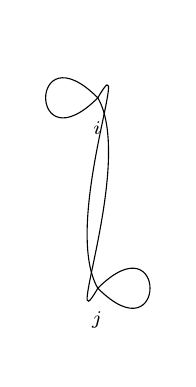
\begin{tikzpicture}[baseline={([yshift=0.2ex]current bounding box.center)}]
      \begin{feynman}
        \vertex (a);
        \vertex (b);
        \diagram {
          a -- [out=135, in=-135, loop, min distance=1.25 cm] a -- 
          [out=60, in=120] b -- [out=45, in=-45, loop, min distance=1.25cm] b 
          -- [out=-120, in=-60] a,
        };
        \vertex [below=0.5em of a] {\(_{i}\)};  
        \vertex [below=0.5em of b] {\(_{j}\)};  
      \end{feynman}
    \end{tikzpicture}
    + \frac{1}{48} 
    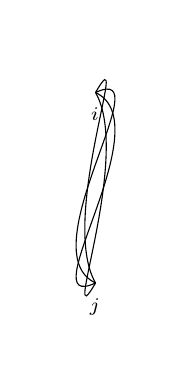
\begin{tikzpicture}[baseline={([yshift=0.2ex]current bounding box.center)}]
      \begin{feynman}
        \vertex (a);
        \vertex (b);
        \diagram {
          a -- 
          [out=60, in=120] b 
          -- [out=-120, in=-60] a,
          a -- [out=25, in=155] b 
          -- [out=-155, in=-25] a,
        };
        \vertex [below=0.2em of a] {\(_{i}\)};  
        \vertex [below=0.2em of b] {\(_{j}\)};  
      \end{feynman}
    \end{tikzpicture}
    \right]\, .
\end{align}
It it clear from the diagrammatic representation that we can
distinguish connected and disconnected contributions. The connected
contributions are represented by connected diagrams, i.e. diagrams
that are made of a single line. The disconnected diagrams are products
of multiple connected parts, and therefore correspond to products of
independent sums over subset of indices. In
Eq.~\ref{eq:PhiFourPartitionFuncOrderLambdaTwo} only the first term in
the bracket in the second line is a disconnected contribution. 

\paragraph{Connected contribution}

Using the Taylor expansion for the logarithm,
\begin{equation}
  \label{eq:TaylorLog}
  \log(1+x) = \sum_{n=1}^\infty (-)^{n+1} \frac{x^n}{n}\, ,
\end{equation}
we can compute
\begin{align}
  \label{eq:PhiFourPartitionFuncConnectOrderLambdaTwo}
  \log\left(Z(\lambda)/Z(0)\right) = 
                    &- \lambda \frac{1}{8} \sum_{i=1}^n \Delta_{ii}^2
                                     +\nonumber \\
                     &+\lambda^2
                    \left[
                    \frac{1}{128} \sum_i \Delta_{ii}^2 \sum_j \Delta_{jj}^2 +
                    \frac{1}{16} \sum_{ij} \Delta_{ii} \Delta_{jj} \Delta_{ij}^2 +
                    \frac{1}{48} \sum_{ij} \Delta_{ij}^4
                    \right] -  \nonumber \\
  &- \lambda^2 \frac{1}{2} \left( - \frac{1}{8}
    \sum_{i=1}^n \Delta_{ii}^2\right)^2 +  O(\lambda^3)\, . 
\end{align}
Eq.~\ref{eq:PhiFourPartitionFuncConnectOrderLambdaTwo} shows
explicitly the cancellation at order $\lambda^2$ between the first
term in the square bracket in the second line, and the last term in
the third line, which comes from squaring the order $\lambda$
contribution when computing the second term in the Taylor expansion in
Eq.~\ref{eq:TaylorLog}. This is a general property, taking the
logarithm of the generating function yields the generating function of
connected conributions. We shall prove this property later in the
course. 

\section{Perturbed Gaussian Correlators}
\label{sec:pert-gauss-corr}

The perturbative treatment discussed above can be extended to compute
moments of the distribution:
\begin{equation}
  \label{eq:lPointCorrPert}
  \langle x_{i_1} \ldots x_{i_\ell}\rangle =
  \frac{1}{Z(\lambda)} 
  \int d^nx\, e^{-S(x;\lambda)} x_{i_1} \ldots x_{i_\ell}\, ,
\end{equation}
which often referred to as an $\ell$-point correlator/function. Let us start
our discussion with a simple example. 

\paragraph{Two-point function}

We need to evaluate
\begin{align}
  \int d^nx\, e^{-S(x;\lambda)} x_{i_1} x_{i_2} &= 
  \int d^nx\, e^{-S_0(x;\lambda)}\, \left[\sum_{k=0}^\infty
  \frac{(-)^k}{k!} \lambda^k V(x)^k \right]\, x_{i_1} x_{i_2} \\
  \label{eq:TwoPointCorrPert}
                                               &=Z(0) \sum_{k=0}^\infty
  \frac{(-)^k}{k!} \lambda^k \langle V(x)^k x_{i_1} x_{i_2}\rangle_0\, ,
\end{align}
where in the second line we have expressed the initial correlator in
terms of correlators computed in the Gaussian theory, denoted as
before by $\langle \ldots \rangle_0$. The Gaussian correlators can be
computed using Wick's theorem as before. We shall consider again a
quartic potential:
\begin{equation}
  V(x) = \frac{1}{4!} \sum_{i=1}^n x_i^4\, ,
\end{equation}
and compute all the terms in Eq.~\ref{eq:TwoPointCorrPert} order by
order in $\lambda$ up to order $\lambda^2$.
\begin{itemize}
\item $O(\lambda^0)$ For $k=0$ we simply get the two-point Gaussian
  correlator: 
  \begin{align}
    \langle x_{i_1} x_{i_2} \rangle_0 = \Delta_{i_1 i_2}\, .
  \end{align}
\item $O(\lambda^1)$ At first order in $\lambda$ we have one insertion
  of $V$:
  \begin{align}
    \langle V(x) x_{i_1} x_{i_2} \rangle_0 = \frac{1}{4!} \sum_{i=1}^n
    \langle x_i^4 x_{i_1} x_{i_2} \rangle_0\, .
  \end{align}
  This Gaussian expectation value involving six factors of $x$ (four
  from the potential, and the two coming from the fact that we compute
  a two-point function) can be evaluated using Wick's
  theorem. There two types of contractions.
  \begin{itemize}
  \item [(i)] $x_1$ is contracted with $x_2$, and the four $x_i$ are
    contracted amongst themselves:
    \begin{align}
      \contraction{}{x_{i_1}}{}{x_{i_2}}
      x_{i_1} x_{i_2} 
      \left(
      \contraction{}{x_{i}}{}{x_{i}}
      \contraction{x_{i} x_{i}}{x_{i}}{}{x_{i}}
      x_{i} x_{i} x_{i} x_{i} +
      \contraction{}{x_{i}}{x_{i}}{x_{i}}
      \contraction[2ex]{x_{i}}{x_{i}}{ x_{i}}{x_{i}}
      x_{i} x_{i} x_{i} x_{i} +
      \contraction{}{x_{i}}{x_{i}x_{i}}{x_{i}}
      \contraction[2ex]{x_{i}}{x_{i}}{}{x_{i}}
      x_{i} x_{i} x_{i} x_{i} 
      \right) = \Delta_{i_1 i_2} \langle x_i^4\rangle_0
      \, ,
    \end{align}
    where we have used the fact that the term inside the bracket on
    the LHS is simply $\langle x_i^4\rangle_0$ --
    cfr. Eq.~\ref{eq:FourPtGaussContract}.
  \item [(ii)] $x_1$ and $x_2$ are contracted with some of the $x_i$;
    there are 12 such contractions:
    \begin{align}
      \contraction{}{x_{i_1}}{x_{i_2}}{x_{i}}
      \contraction[2ex]{x_{i_1}}{x_{i_2}}{x_{i}}{x_{i}}
      x_{i_1} x_{i_2}  x_{i} x_{i} x_{i} x_{i} + \ldots = 
      \Delta_{i i_1} \Delta_{i i_2} \Delta_{i i} \times 4
      \times 3\, .
    \end{align}
  \end{itemize}
  Collecting all terms yields
  \begin{align}
   \frac{1}{4!} \sum_{i=1}^n
    \langle x_i^4 x_{i_1} x_{i_2} \rangle_0 = 
    \Delta_{i_1 i_2} \frac{1}{4!} \sum_{i=1}^n \langle x_i^4\rangle_0
    + \frac{1}{4!} \times 4 \times 3 \sum_{i=1}^n \Delta_{i i_1}
    \Delta_{i i_2} \Delta_{i i} \, .
  \end{align}
\item $O(\lambda^2)$ At this order we need to evaluate
  \begin{align}
    \frac{1}{2!} \langle V(x)^2 x_{i_1} x_{i_2} \rangle_0 = 
    \frac{1}{2!} \frac{1}{(4!)^2} \sum_{i,j=1}^n \langle x_i^4 x_j^4
    x_{i_1} x_{i_2} \rangle_0\, .
  \end{align}
  There are five different types of contractions, each of them coming
  with a given multiplicity. We encourage the interested reader to
  compute those contributions, and check carefully that the correct
  multiplicities are recovered. 
\end{itemize}
Collecting all contributions yields
\begin{align}
  \int d^nx\, e^{-S(x;\lambda)} 
  x_{i_1} x_{i_2} = Z(0) & 
                           \left[
                           \Delta_{i_1 i_2} - \lambda \left(\Delta_{i_1 i_2}
                           \frac{1}{4!} \sum_{i=1}^n \langle
                           x_i^4\rangle_0 +  \frac12 \sum_{i=1}^n
                           \Delta_{i i_1} \Delta_{i i_2} \Delta_{i i} 
                           \right) + \right. \nonumber \\
                         & \left.
                           + \lambda^2 \left( 
                           \frac{1}{2!} \Delta_{i_1 i_2} \frac{1}{(4!)^2}
                           \sum_{i,j=1}^n \langle x_i^4 x_j^4 \rangle_0
                           + \frac{1}{2!} \sum_{i=1}^n \Delta_{i i_1}
                           \Delta_{i i_2} \Delta_{i i}  \frac{1}{4!}
                           \sum_{j=1}^n \langle x_j^4 \rangle_0
                           + \right. \right. \nonumber \\
                         & + \left. \left.
                           \frac{1}{4} \sum_{i,j=1}^n \Delta_{i i_1}
                           \Delta_{i i_2} \Delta_{i j}^2 \Delta_{jj}
                           + \frac{1}{6} \sum_{i,j=1}^n \Delta_{i i_1}
                           \Delta_{j i_2} \Delta_{i j}^3 +
                           \right. \right. \nonumber \\
  \label{eq:TwoPointNotNorm}
                         & + \left. \left.
                           \frac{1}{4} \sum_{i,j=1}^n \Delta_{i i_1}
                           \Delta_{j i_2} \Delta_{i j} \Delta_{ii}\Delta_{jj}
                           \right)
                           \right]\, .
\end{align}
Diagrammatically we have: 
\begin{align}
  \label{eq:TwoPtVacuumIncluded}
  \langle x_{i_1} x_{i_2}\rangle = 
  \frac{Z(0)}{Z(\lambda)} \Bigg[
    \begin{tikzpicture}[baseline={([yshift=1.4ex]current bounding box.center)}]
    \begin{feynman}[inline=(a)]
      \vertex (a);
      \vertex (b);
      \diagram {
        a -- b,
      };
      \vertex [below=0.2em of a] {\(_{i_1}\)};  
      \vertex [below=0.2em of b] {\(_{i_2}\)};  
    \end{feynman}
  \end{tikzpicture}
  + \frac{\lambda}{8}
    \begin{tikzpicture}[baseline={([yshift=-5ex]current bounding box.center)}]
    \begin{feynman}[layered layout, vertical'=i to c]
      \vertex (a);
      \vertex (c); 
      \vertex (b);
      \vertex (i);
      \vertex (j);
      \vertex (k);
      \diagram {
        j -- [draw=none]  i -- [draw=none] k, 
        i -- [out=45, in=-45, loop, min distance=2cm] i --
        [out=135, in=-135, loop, min distance=2 cm] i,
        a -- c -- b, 
        c --[opacity=0.1] i, 
      };
      \vertex [below=0.2em of a] {\(_{i_1}\)};  
      \vertex [below=0.2em of b] {\(_{i_2}\)};  
%      \vertex [below=0.2em of c] {\(c\)};  
      \vertex [below=0.2em of i] {\(_{i}\)};  
    \end{feynman}
  \end{tikzpicture}
  + \frac{\lambda}{2}
    \begin{tikzpicture}[baseline={([yshift=-3ex]current bounding box.center)}]
    \begin{feynman}[layered layout, vertical'=i to c]
      \vertex (a);
      \vertex (b);
      \vertex (i);
      \diagram {
        a -- i -- b, 
        i -- [out=135, in=45, loop, min distance=2cm] i,
      };
      \vertex [below=0.2em of a] {\(_{i_1}\)};  
      \vertex [below=0.2em of b] {\(_{i_2}\)};  
%      \vertex [below=0.2em of c] {\(c\)};  
      \vertex [below=0.2em of i] {\(_{i}\)};  
    \end{feynman}
  \end{tikzpicture}
  + O(\lambda^2)
  \Bigg]\, ,
\end{align}
where for simplicity we have omitted the contribution of order
$\lambda^2$. A diagram that can be factorised as the product of a
subdiagram with external lines and a subdiagram that is made of loops
only is called a {\em vacuum contribution}. For instance the second
diagram inside the bracket in Eq.~\ref{eq:TwoPtVacuumIncluded} is a
vacuum contribution, while the first and third ones are not.

Finally, we need to divide this expression by $Z(\lambda)$ in order to
obtain the two-point correlator as defined in
Eq.~\ref{eq:lPointCorrPert}.  As a result, we obtain a factor of
$Z(0)/Z(\lambda)$ multiplying the expression inside the square bracket
in Eq.~\ref{eq:TwoPointNotNorm}. Inverting
Eq.~\ref{eq:PhiFourPartitionFuncOrderLambdaTwo} for the ratio
$Z(0)/Z(\lambda)$ yields
\begin{align}
 Z(0)/Z(\lambda) &= 
                    1 + \frac{1}{4!} \lambda \sum_{i=1}^n \langle x_i^4\rangle_0 
                    - \frac{1}{2!} \frac{1}{(4!)^2} \lambda^2 \sum_{i,j=1}^n 
                    \langle x_i^4 x_j^4\rangle_0 
                   + \frac{1}{(4!)^2} \lambda^2 \left(\sum_{i=1}^n \langle x_i^4\rangle_0\right)^2
                   + O(\lambda^3) 
\end{align}

\begin{Ex}
  Show that all the vacuum contributions cancel when computing $\langle
  x_{i_1} x_{i_2}\rangle$. The final result is
  \begin{align}
  \int d^nx\, e^{-S(x;\lambda)} 
  x_{i_1} x_{i_2} = Z(0) & 
                           \left[
                           \Delta_{i_1 i_2} - \lambda  \frac12 \sum_{i=1}^n
                           \Delta_{i i_1} \Delta_{i i_2} \Delta_{i i} 
                            + \right. \nonumber \\
                         & \left.
                           + \lambda^2 \left( 
                           \frac{1}{4} \sum_{i,j=1}^n \Delta_{i i_1}
                           \Delta_{i i_2} \Delta_{i j}^2 \Delta_{jj}
                           + \frac{1}{6} \sum_{i,j=1}^n \Delta_{i i_1}
                           \Delta_{j i_2} \Delta_{i j}^3 +
                           \right. \right. \nonumber \\
  \label{eq:TwoPointNorm}
                         & + \left. \left.
                           \frac{1}{4} \sum_{i,j=1}^n \Delta_{i i_1}
                           \Delta_{j i_2} \Delta_{i j} \Delta_{ii}\Delta_{jj}
                           \right)
                           \right]\, .
\end{align}
Write a diagrammatic representation for the contributions $O(\lambda^2)$.
\end{Ex}
This is a general property: when the integral is divided by the
correct normalization factor $1/Z(\lambda)$, all vacuum contributions
cancel.

\section{Generating Functions for the Perturbed Gaussian Measure}
\label{sec:gener-funct-pert}

\paragraph{Correlators}

We can now generalise the idea of a generating function to the case of
a non Gaussian measure. Introducing
\begin{equation}
  \label{eq:GenFunctPert}
  Z(b;\lambda) = \int d^nx\, \exp\left[
    -S(x;\lambda) + (b,x)
    \right]\, ,
\end{equation}
where we introduced the notation
\begin{equation}
  \label{eq:ScalProd}
  (b,x) = \sum_{i=1}^n b_i x_i\, .
\end{equation}
Note that we can also write
\begin{equation}
  \label{eq:GenFunctPertTwo}
  \langle e^{(b,x)} \rangle = Z(b;\lambda)/Z(\lambda)\, .
\end{equation}
The correlators in the perturbed measure are obtained by
differentiation
\begin{equation}
  \label{eq:CorrGenPert}
  \langle x_{i_1} \ldots x_{i_\ell}\rangle = \frac{1}{Z(\lambda)} \left.
  \frac{\partial}{\partial b_{i_1}} \ldots \frac{\partial}{\partial b_{i_\ell}}\,
  Z(b;\lambda)
\right|_{b=0} \, .
\end{equation}

\paragraph{Cumulants}

The logarithm of $Z(b;\lambda)$ is usually denoted $W(b;\lambda)$, 
\begin{equation}
  \label{eq:WGenDef}
  Z(b;\lambda) = e^{W(b;\lambda)}\, ;
\end{equation}
$W(b;\lambda)$ is the generator is the generator of the connected
$\ell$-point correlators, $W_{i_1 \ldots i_\ell}$, i.e. the correlators that can be represented as a single
diagram, with $\ell$ open ends:
\begin{equation}
  \label{eq:DiffWGen}
  W_{i_1 \ldots i_\ell} = \left.
  \frac{\partial}{\partial b_{i_1}} \ldots \frac{\partial}{\partial b_{i_\ell}}\,
  W(b;\lambda)
\right|_{b=0} \, .
\end{equation}
In statistics, the $W_{i_1 \ldots i_\ell}$ are called the {\em
  cumulants} of the probability distribution $e^{-S(x;\lambda)}$.





\chapter{Distributions}
\label{chap:distr-notes}
\section{Definitions}
\label{sec:distr-defs}

We collect here a quick summary of definitions and properties of distributions.
These are commonly used in QFT -- often without paying too much attention to
them. 

\begin{Def}
    A {\em distribution} is a continuous linear functional on a space of 
    test functions. 
\end{Def}
The space of test functions may vary. We will mostly focus on {\em tempered}
distributions, \ie distributions that act on
$\mathcal{S}\left(\mathbb{R}^n\right)$, the space of complex-vaued, infinitely
differentiable functions, which, together with their derivatives, approach zero
at infinity, faster than any inverse power of the Euclidean distance. In order
to make this statement mathematically precise, we need to introduce some
notation. We denote by $k$ a generic $n$-tuple of integers, 
\begin{equation}
    \label{eq:MultiIndexDef}\
    k = \left\{ k_1, \ldots k_n\right\}\, ,
\end{equation}
then 
\begin{align}
    \label{eq:modk-def}
    |k| &= k_1 + \ldots + k_n\, , \\
    \label{eq:x-power-k}
    x^k &= x_1^{k_1} \ldots x_n^{k_n}\, , \\
    \label{eq:factk-def}
    k! &= k_1! \ldots k_n!\, , \\
    \label{eq:dx-def}
    dx &= \prod_{i=1, \ldots, n} dx_i\, , \\
    \label{eq:derivs}
    D^k &= \frac{\partial^{|k|}}{\partial x_1^{k_1} \ldots \partial x_n^{k_n}}\, .
\end{align}
For each pair of integers, $(r,s)$, a norm can be defined for functions in
$\mathbb{R}^n$,
\begin{Def}
    \[
    ||f||_{r,s} = \sum_{|k|\leq r} \sum_{|l|\leq s} \, 
    \sup_{x\in \Rn} \left| x^k D^l f(x)\right| \, .
    \]
\end{Def}
The set of tempered functions is the set of functions with finite norm, 
\[
    f \in \mathcal{S}(\Rn) \quad 
    \Longleftrightarrow \quad
    ||f||_{r,s} < \infty\, , \quad \forall r,s \in \mathbb{N}\, .    
\]
We can now introduce the concept of convergence in $\mathcal{S}$.
\begin{Def}
    The series $\{f_m\}$ converges to $f$, 
    \[
        \lim_{m\to\infty} f_m = f\, , \quad \mathrm{if} \ 
        \lim_{m\to\infty} ||f_m -f||_{r,s} = 0 \, .
    \] 
\end{Def}
Finally, we can define the notion of continuity for functionals acting on
$\mathcal{S}$. A {\em tempered distribution} $T$ is continuous in $\mathcal{S}$,
\ie
\[
    \lim_{m\to\infty} ||f_m - f||_{r,s} \quad
    \Longrightarrow \quad
    \lim_{m\to\infty} |Tf_m - Tf| = 0\, .
\]
Note that a necessary and sufficient condition for continuity is 
\[
    |Tf| \leq C ||f||_{r,s}\, , 
    \quad \mathrm{for\ some\ values\ of}\ r,s\, .    
\]
A very useful result states that every tempered distribution can be written as
\begin{align}
    \label{eq:TempConv}
    Tf 
        &= \sum_{|k|\leq s} \int dx\, 
            F_k(x_1 \ldots x_n) D^k f(x_1 \ldots x_n) \\
        &= \int dx\, T(x) f(x)\, ,
\end{align}
where $k$ is a multi-index as defined in Eq.~\eqref{eq:MultiIndexDef}, and the
coefficients $F_k$ are continuous functions that satisfy
\begin{equation}
    \label{eq:FkBound}
    \left|F_k(x)\right| \leq C_k \left(1 + |x|^j\right)\, ,
\end{equation}
for some $j$ that depends on $k$. We integrate by parts (when possible) and
write
\begin{align}
    \label{eq:TempKernel}
    T(x) = \sum_{|k|\leq s} (-)^{|k|} D^k F_k(x)\, .
\end{align}
The set of tempered distributions is denoted $\mathcal{S}'$. At times we will
encounter distributions that do not belong to $\mathcal{S}'$, but to the larger
set $\mathcal{D}'$, of linear continuous functionals acting on $\mathcal{D}$,
the space of infinitely differentiable functions with compact support in $\Rn$.
Clearly $\mathcal{D}\subset\mathcal{S}$ and therefore $\mathcal{S}' \subset
\mathcal{D}'$. Examples of elements of $\mathcal{D}'$ that do not belong to
$\mathcal{S}'$ are exponentially growing functions, or 
\[
    T(x) = \sum_{m=0}^\infty \delta^{(m)}(x-m)\, .   
\]

\section{Miscellaneous Properties}
\label{sec:MiscProp}

Let us consider invertible inhomogeneous transformations in $\Rn$
\begin{equation}
    \label{eq:RnInhomogeneous}
    \{a, L\}:\, x \mapsto L x + a\, ,
\end{equation}
for any function $f\in\mathcal{S}$, we define the {\em shifted} function
\begin{equation}
    \label{eq:ShiftedFun}
    \left(\{a,L\} f\right)(x) = 
        f\left(L^{-1}(x-a)\right)\, .
\end{equation}
The shifted distribution in $\mathcal{S}'$ is defined by
\begin{equation}
    \label{eq:ShiftedDistr}
    T_{\{a,L\}} f = \left|\det L\right|^{-1} 
        T\left(\{a,L\}f\right)\, .
\end{equation}
If $T$ is a function
\begin{equation}
    \label{eq:ShiftedDistrFun}
    T_{\{a,L\}}(x) = T(Lx+a)\, .
\end{equation}

The derivatives of a distribution are defined by the relation
\begin{equation}
    \label{eq:DistrDeriv}
    D^p T(f) = (-)^{|p|}\, T\left(D^pf\right)\, .
\end{equation}
Note that using the definition in Eq.~\eqref{eq:ShiftedDistr}, the derivative of
a distribution can be equivalently defined as
\begin{equation}
    \label{eq:EquivDerivDef}
    \frac{\partial}{\partial x_j} T (f) =
    \lim _{a_j\to 0} \frac{1}{a_j} \left(T_{\{a_j\}} - T\right)(f)\, .
\end{equation}
We do not want to write a book on distributions here, so we will not dwell on
proving nice identities. Instead we refer the reader to the book by Streater \&
Wightman for the details.  

Multiplication by a function, tensor product of distributions, and convolution
with a function can be defined in the {\em obvious} way. The only subtlety to
keep in mind is that when we multiply a tempered distribution by a generic,
infinitely differentiable function $g$, the result may not be a tempered
distribution. In order to guarantee that we recover a tempered distribution, we
need to require $g$ and all its derivatives are bounded by polynomials. 

\paragraph{Nuclear Theorem}

It is necessary at times to consider multilinear functionals that are separately
continuous in all their arguments. An obvious way to construct such
distributions is to consider a distribution $G$ in all the variables together,
and specialize it to test functions that are products $f_1(x_1) \ldots
f_m(x_m)$. The nuclear theorem found by Schwartz guarantees that these are the
only possible distributions. 
\begin{Thm}
    Let $T$ be a multilinear functional of arguments 
    $f_1, \ldots, f_m \in \mathcal{S} (\in \mathcal{D})$, which is continuous in 
    each of its arguments while the others are fixed, then there exists a unique 
    distribution $G \in \mathcal{S}' (\in \mathcal{D}')$ such that
    \[
        T(f_1, \ldots, f_m) = G(f_1 \ldots f_m)\, .    
    \]
\end{Thm}

\section{Fourier Transforms}
\label{sec:FTDistr}

Let us recall briefly the conventions used here for the Fourier transform. In
Euclidean space, we use
\begin{align}
    P_k = -i \partial_k 
    \quad \Longrightarrow \quad 
    \braket{x}{p} = e^{i p\cdot x}\, .
\end{align}
The Fourier transform is 
\begin{align}
    \left(\mathcal{F}f\right)(p) 
        &= \braket{p}{f} = \int d^Dx\, \braket{p}{x} \braket{x}{f} \\
        &= \int d^Dx\, e^{-i p\cdot x} f(x)\, ,
\end{align}
and similarly for the inverse transform
\begin{align}
    \left(\bar{\mathcal{F}} f\right)(x) = 
    \int \frac{d^Dp}{(2\pi)^D}\, e^{i p\cdot x} 
    f(p)\, .
\end{align}
With these conventions
\begin{align}
    \mathcal{F} \bar{\mathcal{F}} =
    \bar{\mathcal{F}} \mathcal{F} = 
    1\, .
\end{align}
Using these definitions we have
\begin{equation}
    \label{eq:Fdkf}
    \mathcal{F}\left(D^kf\right)(p) = 
        \left(ip\right)^k \left(\mathcal{F}f\right)(p)\, .
\end{equation}

\begin{Def}
    The Fourier transform of a distribution $T$ is defined by imposing
    \begin{equation}
        \label{eq:FTDistrDef}
        \left(\mathcal{F}T\right) (f) = 
        T\left(\mathcal{F}f\right)\, .
    \end{equation}
\end{Def}

\begin{Ex}
    Show that with the definitions above
    \begin{align}
        \mathcal{F}[\delta(x)] 
            &= 1\, ,    \\
        \mathcal{F}[e^{ikx}] 
            &= (2\pi) \delta(p-k)\, \quad \forall k \in \mathbb{R}\, .
    \end{align}
    where $\delta(x)$ is Dirac's delta function (which is actually a
    distribution). Check that you can generalize these expressions to the case
    of $x,p \in \Rn$.
\end{Ex}

\section{Laplace Transform}
\label{sec:LaplaceTransf}

\begin{Def}
    The Laplace transform of a function $f\in \mathcal{S}(\mathbb{R})$ is 
    defined as
    \begin{align}
        \label{eq:LaplaceTransfDef}
        g(z) = \int_0^\infty dk\, e^{i k (x+iy)} f(k)\, , \quad z=x+iy\, .
    \end{align}
\end{Def}
The function $g(z)$ is holomorphic in the plane $y>0$. This definition can be
generalized to the case of multiple variables, where the integral over the
positive $k$ axis is replaced by an integral in a {\em convex cone}. We admit
distributions as boundary values of these Laplace transforms. The generalization
of the upper half-plane is a so-called {\em tube}, where the imaginary parts of
the complex variables are constrained to be in a cone. In the multi-dimensional
case, we can extend the definition of holomorphic function as follows. 

\begin{Def}
    A function $f$, defined in a neighbourhood of $w \in \Cn$, is {\em
    holomorphic} (or analytic) at the point $w$ if there exists a series
    \begin{align}
        \label{eq:HoloSeriesDef}
        \sum_{k_1, \ldots, k_n=0}^\infty &a_{k_1 \ldots k_n} (z_1-w_1)^{k_1} \ldots
            (z_n - w_n)^{k_n} \\
        & \sum_k a_k (z-w)^k\, ,
    \end{align}
    which converges for $z$ in a neighbourhood of $w$, and is equal to $f(w)$
    when $z=w$. 
\end{Def}
Note that the second line is a compact rewriting of the first one using the
multi-index notation. If the series converges at $z$, then it converges
absolutely and uniformly in the polydisc
\begin{align}
    \left| \zeta_j - w_j \right| \leq |z_j - w_j| - \epsilon\, .
\end{align}
The coefficients are obtained by differentiating the function at $w$, 
\begin{align}
    \label{eq:CoeffsFromDerivs}
    a_{k_1\ldots k_n} = 
        \left. \frac{1}{k!} D^{k}f(z_1, \ldots, z_n) \right|_{w_1=z_1 \ldots w_n=z_n}\, .
\end{align}
Cauchy's formula yields
\begin{align}
    f(z_1, \ldots, z_n) = \frac{1}{(2\pi i)^n} \int_{R_1} \ldots \int_{R_n}
        d\zeta_1 \ldots d\zeta_n\,  
        \frac{f(\zeta_1, \ldots, \zeta_n)}{(\zeta_1 - z_1) \ldots (\zeta_n - z_n)}\, , 
\end{align}
inside a polydisc of uniform convergence. Holomorphic functions of several
variables can be extended by analytical continuation. The coefficients of the
power series that defines a holomorphic function can be obtained by computing
the derivatives along the real axis, \ie by varying only the real part of the
complex arguments. 

A holomorphic function $F$ defined in an open set $\mathcal{O}$ is a
distribution in $\mathcal{D}(\mathcal{O})'$. If $T$ is a distribution in
$\mathcal{D}_p'$, it may happen that $e^{-\eta \cdot p} T$ is a distribution in
$\mathcal{S}_p'$. Then we can define the Laplace transform of $T$ as the
distribution
\begin{align}
    \label{eq:LaplaceDistrDef}
    \mathcal{L}(T) = \mathcal{F}\left(e^{\eta\cdot p} T\right)\, .
\end{align}
For a function $T$ we get
\begin{align}
    \label{eq:LaplaceDistrFunc}
    \mathcal{L}(T)(\xi,\eta) = 
        \int \frac{d^Dp}{(2\pi)^D}\, e^{-i p (\xi - i \eta)} T(p)\, .
\end{align}
Here there are no requirements on the support of $T$; this is called a two-sided
Laplace transform. The one-dimensional definition in
Eq.~\eqref{eq:LaplaceTransfDef} is a special case of this more general
definition. 

\subsection{Properties}
\label{sec:LaplaceProperties}

We list here some useful properties, without getting into the details of the
proofs.

\begin{Thm}
    Let $T \in \mathcal{D}_p'$, the set of all $\eta$ such that 
    $e^{-p\cdot \eta} T \in \mathcal{S}_p'$ is {\em convex}.
\end{Thm}
The proof is very nice, but we do not have time for it right now. See Thm. 2.5
in Streater \& Wightman for the details. 

\begin{Thm}
    Let $\Gamma$ be a convex open set in $\Rn$, $T \in \mathcal{D}_p'$ such that
    \[
        \forall \eta \in \Gamma\, , e^{-\eta\cdot p} T \in \mathcal{S}_p'\, ,   
    \]
    then $\mathcal{L}(T)$ is a holomorphic function of $\xi-i\eta$ in the tube
    $\Rn - i\Gamma$. $\mathcal{L}(T)$ satisfies
    \begin{align}
        \label{eq:PolyBound}
        |\mathcal{L}(T)(\xi-i\eta)| \leq \left|P_k(\xi)\right|\, ,           
    \end{align}
    where $P_k$ is a polynomial, and $\eta$ varies over any compact 
    subset $K \subset\Gamma$.

    Conversely, every function holomorphic in the tube, and satisfying the bound
    in Eq.~\eqref{eq:PolyBound} is the Laplace transform of a uniquely
    determined $T \in \mathcal{D}_p'$, such that $e^{-\eta\cdot p} T \in
    \mathcal{S}_p'$ for all $\eta\in\Gamma$.
\end{Thm}

\begin{Thm}
    \label{thm:TranslationTube}
    Let $T\in\mathcal{D}_p'$ and $\Gamma\in\Rn$, convex, such that 
    \[
        \forall\eta\in\Gamma\, , e^{-p\cdot\eta} T \in \mathcal{S}_p'\, .    
    \]
    If $T$ has its support in a half-space such that $p\cdot a > A$, then
    $\Gamma$ contains all the points of the form $\eta + t a$, with $t\geq 0$.
\end{Thm}

The `plus' lightcone, $V_+$, is defined as the set of $D$-momenta $p$ such that
\begin{align}
    \label{eq:PlusLightConeDef}
    p^2 = (p^0)^2 - \mathbf{p}^2 > 0\, , \quad p^0 > 0\, .
\end{align}
Its closure is denoted $\bar{V}_+$. In QFT we find distributions $T$ that are
functions of $n$ $D$-momenta $p_1,\dots, p_n$. These distributions vanish if
some momentum $p_i$ is outside $\bar{V}_+$, and are also tempered. Using
Theorem~\ref{thm:TranslationTube}, we deduce that $\mathcal{L}(T)(\xi-ia)$ is
analytic in the {\em tube}:
\begin{align}
    \label{eq:ForwardTube}
    \mathcal{T}_n=\Rn - i\Gamma\, ,
\end{align}
where
\[
    \Gamma = \left\{
        (a_1, \ldots a_n)\, , \, a_j \in V_+\, , \, j=1, \ldots n
    \right\}\, .    
\]
Note that here we use the fact that if $p,q \in V_+$, then $p\cdot q > 0$. 
For functions that have support in the cone $\mathcal{T}_n$, we have the 
following property. 

\begin{Thm}
    Let $T \in \mathcal{D}_p'$ and $e^{-p\cdot\eta} T \in\mathcal{S}_p'$ 
    for $\eta\in\Gamma$, where $\Gamma$ is the cone $\eta_j\in V_+$ for 
    $j=1, \ldots, n$. Let also 
    \begin{equation}
        p \in \mathrm{supp}\ T 
        \quad \Longrightarrow \quad
        p_j \in V_+\, , j=1, \ldots, n\, .    
    \end{equation}
    Then for each $\eta\in\Gamma$, there is a polynomial $P_\eta$ 
    such that
    \begin{align}
        \label{eq:InequalityAbove}
        |\mathcal{L}(T)\left(\xi - i (\eta+a)\right)|
        \leq |P_\eta(\xi-ia)|\, ,
    \end{align}
    for all $\xi$ and all $a\in\Gamma$.

    Conversely, if $F$ is holomorphic in $\mathcal{T}_n$ and 
    satisfying Eq.~\eqref{eq:InequalityAbove} for each 
    $\eta\in\Gamma$ and some polynomial $P_\eta$, then $F$ is the 
    Laplace transform of a distribution with support in $\Gamma$.
\end{Thm}

The existence of a boundary value of Laplace transforms is dictated
by the following theorem. 
\begin{Thm}
    If $T\in\mathcal{S}_p'$ and $\mathcal{L}(T)$ exists for all $\eta\in\Gamma$, 
    then
    \begin{align}
        \label{eq:BoundaryValueThm}
        \lim_{\eta\to 0} \int d\xi\, \mathcal{L}(T)(\xi-i\eta) f(\xi) 
        = \mathcal{F}(T)(f)\, ,
    \end{align}
    \ie $\mathcal{L}(T)$ converges in $\mathcal{S}_p'$ to $\mathcal{F}(T)$ 
    as $\eta\to 0$ inside a cone $\Gamma$.

    Conversely if $\mathcal{L}(T)$ converges in $\mathcal{S}_\xi'$ as $\eta\to 0$
    in a cone $\Gamma$, then $T$ is the Laplace transform of a tempered distribution.
\end{Thm}

\section{Extended Tubes}
\label{sec:ExtTubes}

The {\em extended tube}, $\mathcal{T}_n'$, is the union of the open sets
obtained from $\mathcal{T}_n$ by applying proper complex Lorentz
transformations:
\begin{align}
    &\zeta_1, \ldots, \zeta_n \in \mathcal{T}_n' 
    \quad \Longleftrightarrow \quad
    \zeta_1, \ldots, \zeta_n = \Lambda w_1, \ldots, \Lambda w_n\, , \\
    &\quad w_1, \ldots, w_n \in \mathcal{T}_n\, ,  \quad
    \Lambda \in L_+(\mathbb{C})\, . \nonumber
\end{align}
The holomorphic functions that we find in QFT transform according to
some representation $S(A)$ of $\mathrm{SL}(2,\mathbb{C})$:
\begin{align}
    \label{eq:TransfPropFunc}
    f_\alpha(\Lambda(A)\zeta_1, \ldots, \Lambda(A)\zeta_n) =
    S(A)_{\alpha\beta} f_\beta(\zeta_1, \ldots, \zeta_n)\,.
\end{align}
The main result about extended tubes in Streater \& Wightman is the following
theorem.
\begin{Thm}
    If $f_\alpha(\zeta_1, \ldots, \zeta_n)$ transforms according to 
    Eq.~\eqref{eq:TransfPropFunc} and is holomorphic in the tube 
    $\eta_j \in V_+$, where $\zeta_j=\xi_j-i\eta_j$, $j=1, \ldots, n$, 
    then $f_\alpha$ possesses a single-valued analytical continuation
    into the extended tube $\mathcal{T}_n'$.
\end{Thm}

\paragraph{Jost points}

By definition the tube $\mathcal{T}_n$ does not contain real points, 
since $z \in \mathcal{T}_n$ implies $\mathrm{Im}\ z \in V_+$, and 
therefore $\mathrm{Im}\ z \neq 0$.The extended tube contains real points, 
called {\em Jost points}. 

\begin{Ex}
    For the case of one vector, show that a real point 
    $\zeta \in \mathcal{T}_1'$ if and only if $\zeta^2 < 0$.
\end{Ex}

For the general case, we have a theorem by Jost. 
\begin{Thm}
    A real point $\zeta_1,\ldots,\zeta_n$ is in the extended tube
    $\mathcal{T}_n'$ if and only if all vectors of the form 
    \[
     \sum_{j=1}^n \lambda_j \zeta_j\, , \quad \lambda_j\geq 0\, , \sum_j \lambda_j >0\, ,
    \]
    are space-like.
\end{Thm}

\section{The Edge of the Wedge Theorem}
\label{eq:EdgeOfTheWedge}

For one complex variable there is a proof of the edge of the wedge 
theorem that goes back to Painlev\'e in 1888. 

\begin{Thm}
    Let $F_1$ be a holomorphic function in an open set $D_1$ in the upper half
    plane, with an interval $a<x<b$ as part of its boundary. Let $F_2$ be
    holomorphic in an open set $D_2$ in the lower half-plane, with the interval
    $a<x<b$ as part of its boundary. Suppose 
    \begin{align}
        F_1(x) &= \lim_{y\to 0^+} F_1(x+iy) \nonumber \\
        F_2(x) &= \lim_{y\to 0^+} F_2(x-iy) \nonumber 
    \end{align}
    exist uniformly in $a<x<b$, are continuous and satisfy
    \begin{align}
        F_1(x) = F_2(x)\, , \quad \forall x\in (a,b)\, .
    \end{align}
    Then $F_1$ and $F_2$ are the same holomorphic function on 
    $a<x<b$.
\end{Thm}
The proof is reported in Streater \& Wightman. Add it to the notes at a later
stage. 

\paragraph{Schwarz reflection principle} 

This is a corollary of the theorem above. It can be stated as follows. 

If $F_1$ is holomorphic in $D_1$ and converges uniformly to boundary values for
$a<x<b$ which define a real continuous function, then $F_1$ is holomorphic in
$\bar{D}_1$, and
\begin{equation}
    \label{eq:SchwarzAnalytical}
    F_1(z) = F_1(z^*)^*
\end{equation}
defines its analytical continuation. 

For applications in QFT we need a generalization of the edge of the wedge
theorem to the case of several complex variables and to distributions. We are
not going to report the proofs, as they can be found in Streater \& Wightman. We
only state two theorems, which summarise the properties that we encounter in
QFT. 

\begin{Thm}
    \label{thm:EdgeWedgeMultiDim}
    Let $\mathcal{O}$ be open in $\Cn$, containing an open set $E$ of $\Rn$. 
    Let $\mathcal{C}$ be an open convex cone of $\Rn$. Suppose $F_1$ is 
    holomorphic in
    \begin{equation}
        D_1 = \left(\Rn + i \mathcal{C}\right) \cap \mathcal{O} 
    \end{equation} 
    and $F_2$ in 
    \begin{equation}
        D_2 = \left(\Rn - i \mathcal{C}\right) \cap \mathcal{O} \, .
    \end{equation} 
    Suppose the limits for $x\in E$
    \begin{equation}
        \label{eq:UpperEdgeFun}
        \lim_{y\to 0,\; y\in \mathcal{C}} F_1(x+iy) = F_1(x) 
    \end{equation}
    and
    \begin{equation}
        \label{eq:LowerEdgeFun}
        \lim_{y\to 0,\; y\in \mathcal{C}} F_2(x-iy) = F_2(x) 
    \end{equation}
    exist and are continuous and coincide on $E$, with the limit
    being uniform on $E$. 

    Then there exists a complex neighbourhood $N$ of $E$ and a 
    holomorphic function $G$ which coincides with $F_1$ in $D_1$ 
    and $F_2$ in $D_2$. 
\end{Thm}

A similar theorem is valid even in the case where the boundary 
values do not define a continuous function. 

\begin{Thm}
    \label{thm:EdgeWedgeDistr}
    Let us replace hypotheses~\eqref{eq:UpperEdgeFun} 
    and~\eqref{eq:LowerEdgeFun} with the condition that for every 
    test function of compact support in $E$
    \begin{equation}
        \label{eq:UpperEdgeDistr}
        \lim_{y\to 0,\; y\in \mathcal{C}} 
        \int dx\, F_1(x+iy) f(x) = T(f)
    \end{equation}
    and 
    \begin{equation}
        \label{eq:LowerEdgeDistr}
        \lim_{y\to 0,\; y\in \mathcal{C}} 
        \int dx\, F_2(x-iy) f(x) = T(f)\, ,
    \end{equation}
    where $T$ is a distribution in $\mathcal{D}(E)'$.
\end{Thm}


\chapter{Path Integrals in QM}
\label{chap:lec1}
\newcommand{\epsstep}{\left(e^{-i \hat{H} \epsilon}\right)}

\section{Preliminaries}
\label{sec:preliminaries-1}

In this lecture we introduce Path Integrals in the context of
QM. Despite the simpler setting (QM compared to QFT), all the
important features of Path Integrals will be discussed. We consider a
point particle in one-dimension, and denote by $\hat{Q}$ the position
operator, and by $\ket{q}$ the eigenstate corresponding to the eigenvalue
$q$:
\begin{equation}
  \label{eq:QEigen}
  \hat{Q} \ket{q} = q \ket{q}\, .
\end{equation}
The completeness condition for the states $\ket{q}$ is
\begin{equation}
  \label{eq:qComplete}
  \int dq\, \ket{q}\bra{q} = 1\, .
\end{equation}
The aim of this section is to find an expression for the quantum
amplitude $\braket{q't'}{qt}$ for a system in state $\ket{q}$ at time
$t$ to evolve in state $\ket{q'}$ at time $t'$,
\begin{equation}
  \label{eq:AmplitudeDef}
  \braket{q't'}{qt} = \langle q' | e^{-i \hat{H} (t'-t)}|q\rangle\, ,
\end{equation}
where $\hat{H}$ is the Hamiltonian of the system. 

Alternatively, we can think of $\ket{q,t}$ as the eigenvector of the 
position operator in the Heisenberg representation, 
\begin{align}
  \label{eq:QHeisenberg}
  \hat{Q}_H(t) = e^{i \hat{H} t} \hat{Q} e^{-i \hat{H}t}\, .
\end{align}
Then, letting 
\begin{align}
  \label{eq:HeisenbergEigenvect}
  \ket{q,t} = e^{i \hat{H}t} \ket{q}\, ,
\end{align}
we can easily check that
\begin{align}
  \label{eq:HeisenbergCheck}
  \hat{Q}_H(t) \ket{q,t} = q \ket{q,t}\, ,
\end{align}
and $\braket{q't'}{qt}$ reproduces Eq.~\eqref{eq:AmplitudeDef}.

\section{Setting Up the Path Integral}
\label{sec:setting-up-path}

In order to proceed with the calculation, let us define $T=t'-t$ to be
the size of the time interval, and $\epsilon=T/n$, where $n$ is an
integer. Then 
\begin{align}
  t_0 &= t \\
  t_k &= t_0 + k \epsilon, \quad \text{for}\ k=1, \ldots, n-1 \\
  t_n &= t + n \epsilon = t'\, .
\end{align}
\begin{align}
  \langle q' | e^{-i \hat{H} (t'-t)}|q\rangle &= 
                 \langle q' | e^{-i \hat{H} T} | q\rangle \\
               &= \langle q' | \left(e^{-i \hat{H} \epsilon}\right)
                 \ldots \left(e^{-i \hat{H} \epsilon}\right) |
                 q\rangle\, ,
\end{align}
where the expression in the second line contains $n$ factors. 

Inserting the completeness relation $n-1$ times,
\begin{align}
  \label{eq:AmplitudeStepOne}
  \braket{q't'}{qt} = \int \left(\prod_{k=1}^{n-1}dq_k\right)\,
  \langle q' | \left(e^{-i \hat{H} \epsilon}\right) |q_{n-1}\rangle
  \langle q_{n-1} | \left(e^{-i \hat{H} \epsilon}\right) |
  q_{n-2}\rangle \ldots \langle q_1 | \left(e^{-i \hat{H}
  \epsilon}\right) | q\rangle\, .
\end{align}
For small $\epsilon$ we can expand the exponential to first order and
evaluate the matrix elements:
\begin{align}
  e^{-i \hat{H} \epsilon} &= 1 - i \hat{H} \epsilon + O(\epsilon^2)\\
\hat{H} &= \frac12 \hat{P}^2 + V(\hat{Q})\, ,
\end{align}
From the potential energy we get
\begin{align}
  \langle q_k | V(\hat{Q}) | q_{k-1}\rangle &= V(q_{k-1}) \langle q_k
                                              | q_{k-1} \rangle \\
                                            &= V\left(\frac{q_k +
                                              q_{k-1}}{2}\right)
                                              \delta(q_k-q_{k-1}) \\
                                            & = \int \frac{dp}{2\pi} V\left(\frac{q_k +
                                              q_{k-1}}{2}\right) 
                                              e^{ip (q_k-q_{k-1})}
\end{align}
In order to evaluate the contribution of the kinetic term, we
introduce eigenstates of the momentum operator $\ket{p}$
\begin{align}
  \hat{P} \ket{p} = p \ket{p} \\
  \braket{q}{p} = e^{ipq}\, ,
\end{align}
and use the completeness of the states $\ket{p}$:
\begin{align}
  \langle q_k | \hat{P}^2 | q_{k-1}\rangle = 
  \int \frac{dp_k}{2\pi}\, p^2 e^{ip_k(q_k-q_{k-1})}\, .
\end{align}
Hence
\begin{align}
  \label{eq:EpsStepBraKet}
  \langle q_k | e^{-i\hat{H}\epsilon} | q_{k-1}\rangle = 
  \int \frac{dp_k}{2\pi}\, \exp\left\{i\epsilon \left[
  p_k \frac{q_k-q_{k-1}}{\epsilon} - H\left(p_k,\tilde{q}_k\right)
  \right]
  \right\} + O(\epsilon^2)\, ,
\end{align}
where $\tilde{q}_k=\frac{q_k-q_{k-1}}{2}$. Therefore
\begin{align}
  \braket{q't'}{qt} =& \lim_{n\to\infty} \int 
  \left(\prod_{k=1}^{n-1}dq_k\right)\, 
  \left(\prod_{j=1}^{n} \frac{dp_j}{2\pi}\right)\, \times \nonumber\\
  \label{eq:DiscretePhaseSpaceIntegral}
  &\times \exp \left\{
    i\epsilon \sum_{m=1}^{n} \left[
    p_m \frac{q_m-q_{m-1}}{\epsilon} - H\left(p_m, 
    \tilde{q}_m \right)
    \right]
    \right\}\, ,
\end{align}
where $q_0 = q$, and $q_n = q'$. The limit above defines the {\em
  path integral} evaluation of the quantum amplitude, which we denote 
\begin{align}
  \label{eq:PathIntDefZero}
  \braket{q't'}{qt} = 
  \int_{q,q'} \mathcal{D}q \mathcal{D}p \exp \left\{
  i \int_t^{t'} d\tau\, \left[
  p \dot{q} - H(p,q)
  \right]
  \right\}\, .
\end{align}

It is essential to remark at this stage that we have rewritten
a quantum amplitude as an infinite-dimensional integral. On the LHS
of the equation above we have the scalar product of two states in 
the Hilbert space of quantum states of the theory. On the RHS we 
have expressed this scalar product as the result of an integral. 
In the expression on the RHS there are no physical states, no 
operators; just integration variables. Note that we added the suffix
$q,q'$ to the integral sign, in order to keep track of the value of 
the position variables at the boundaries of the time interval. 

\section{Quadratic P dependence}
\label{sec:quadr-kinet-term}

For hamiltonians like the one above, \ie hamiltonians that are only
quadratic in the momentum $\hat{P}$, the expression above can be
simplified by performing the integral over the momenta $p_j$:
\begin{align}
  \int \frac{dp_k}{2\pi}\, \exp\left\{
  i\epsilon\left[
  p_k \left(\frac{q_k-q_{k-1}}{\epsilon}\right) - \frac12 p_k^2
  \right]
  \right\} = \left(2\pi i \epsilon\right)^{-1/2}\,
  \exp\left\{i\epsilon
  \frac12\left(\frac{q_k-q_{k-1}}{\epsilon}\right)^2\right\}\, .
\end{align}
Using this result, we can rewrite the path integral in
\Eqref{eq:PathIntDefZero} as
\begin{align}
  \label{eq:PathIntDefOne}
  \braket{q't'}{qt} = \lim_{n\to\infty}
  \left(2\pi i \epsilon\right)^{-n/2}\,
  \int \prod_{k=1}^{n-1}dq_k\, 
  \exp \left\{
  i \epsilon \sum_{m=1}^{n}
  \, \left[
  \frac12 \left(\frac{q_m-q_{m-1}}{\epsilon}\right)^2
  -V\left(\frac{q_m+q_{m-1}}{2}\right)
  \right]
  \right\}\, .
\end{align}
Assuming that the limit exists, we have obtained the definition of the
path integral as an integral over the position of the system only: 
\begin{align}
  \label{eq:PathIntDef}
  \braket{q't'}{qt} = 
  \int_{q,q'} \mathcal{D}q \exp \left\{
  i \int_t^{t'} d\tau\,  \mathcal{L}(q,\dot{q})
  \right\}\, ,
\end{align}
where $\mathcal{L}$ is the lagrangian of the system. Note that the
suffix of the integral keeps track of the initial- and final-state
configurations $q$ and $q'$. 

\section{Correlators}
\label{sec:correlators}

We are now going to work out expressions for the matrix element of the
position operator inbetween the initial and final state considered
above. 

\subsection{One-point Function}
\label{sec:one-point-function}

The first example that we are going to consider is the matrix element
\begin{align}
  \label{eq:OnePtDef}
  \langle q't' | \hat{Q}_H(\bar{t}) | q t\rangle = 
  \langle q' | e^{-i \hat{H}(t'-\bar{t})} \hat{Q} e^{-i \hat{H}(\bar{t}-t)}
  | q\rangle\, ,
\end{align}
where we assume $t<\bar{t}<t'$, and we have used
\begin{equation}
  \label{eq:HeisenOpEvol}
  \hat{Q}_H(t) = e^{i\hat{H} t} \hat{Q} e^{-i\hat{H} t}\, .
\end{equation}
Proceeding as we did in the previous section, we can write
\begin{align}
  \label{eq:CorrOne}
  \langle q't' | \hat{Q}_H(\bar{t}) | q t\rangle = 
  \bra{q'} \epsstep \ldots \epsstep \hat{Q} \epsstep \ldots
  \epsstep \ket{q}\, ,
\end{align}
where we assumed that $\bar{t}=t_{\bar k}$, and the first and second ellipses
denote respectively $(n-k)$, and $k$ factors of $\epsstep$. Performing
the same manipulations as before we obtain
\begin{align}
  \langle q't' | \hat{Q}_H(\bar{t}) | q t\rangle =& 
  \lim_{n\to\infty} \int 
  \left(\prod_{k=1}^{n-1}dq_k\right) \, 
  \left(\prod_{k=1}^{n} \frac{dp_k}{2\pi}\right)\, q_{\bar k} \times \\
  &\times \exp \left\{
    i\epsilon \sum_{m=1}^{n} \left[
    p_m \frac{q_m-q_{m-1}}{\epsilon} - H\left(p_m, 
    \frac{q_m+q_{m-1}}{2}\right)
    \right]
    \right\}\, .
\end{align}
Note that now there is an extra factor of $q_{\bar k}$ in the integrand,
corresponding to the insertion of the operator $\hat{Q}_H(\bar{t})$. The
limit above  is denoted
\begin{align}
  \langle q't' | \hat{Q}_H(\bar{t}) | q t\rangle &= 
  \int \mathcal{D}q \mathcal{D}p \, q(\bar{t}) 
  \exp \left\{
  i \int_t^{t'} d\tau\, \left[
  p \dot{q} - H(p,q)
  \right]
  \right\}\\
&= \int_{qq'} \mathcal{D}q \, q(\bar{t}) 
  \exp \left\{
  i \int_t^{t'} d\tau\, \mathcal{L}(q,\dot{q})
  \right\}\, .
\end{align}

\subsection{Two-point function}
\label{sec:two-point-function}

Let us now consider the slightly more complicated case of the matrix
element of the product of two position operators
\begin{align}
  \label{eq:TwoPtDef}
  \bra{q't'} \hat{Q}_H(\bar{t}_1) \hat{Q}_H(\bar{t}_2)\ket{qt}\, , 
\end{align}
where now we assume $\bar{t}_1=t_{\bar k_1}$, $\bar{t}_2=t_{\bar k_2}$,
$t'>\bar{t}_1>\bar{t}_2>t$. We can write this correlator as:
\begin{align}
    \bra{q't'} \hat{Q}_H(\bar{t}_1) \hat{Q}_H(\bar{t}_2)\ket{qt} = 
  \bra{q'} \epsstep \dots \hat{Q} \ldots \hat{Q} \ldots \epsstep
  \ket{q}\, ,
\end{align}
where the three ellipses here denote respectively 
$(n-\bar k_1)$, $(\bar k_1-\bar k_2)$,
and $\bar k_2$ factors of $\epsstep$. Proceeding exactly as above yields: 
\begin{align}
  \label{eq:TwoPtPathInt}
  \bra{q't'} \hat{Q}_H(\bar{t}_1) \hat{Q}_H(\bar{t}_2)\ket{qt} = 
  \int_{qq'} \mathcal{D}q\, q(\bar{t}_1) q(\bar{t}_2) 
  \exp \left\{
  i \int_t^{t'} d\tau\, \mathcal{L}(q,\dot{q})
  \right\}\, .
\end{align}

There is a subtlety here that it is worth noting. The ordering of
times in \Eqref{eq:TwoPtDef} matters, while it clearly does not in the
RHS of \Eqref{eq:TwoPtPathInt} where $q(\bar{t}_1)$ and $q(\bar{t}_1)$
are just integration variables. If $\bar{t}_2>\bar{t}_1$, then the RHS
of \Eqref{eq:TwoPtPathInt} corresponds to
\begin{align}
  \bra{q't'} \hat{Q}_H(\bar{t}_2) \hat{Q}_H(\bar{t}_1) \ket{qt}\, .
\end{align}
Both results can be summarised as
\begin{align}
  \label{eq:TOrderPathInt}
  \bra{q't'} T\left(\hat{Q}_H(\bar{t}_1) \hat{Q}_H(\bar{t}_2)
  \right)\ket{qt} = 
  \int_{qq'} \mathcal{D}q\, q(\bar{t}_1) q(\bar{t}_2) 
  \exp \left\{
  i \int_t^{t'} d\tau\, \mathcal{L}(q,\dot{q})
  \right\}\, ,
\end{align}
where we have introduced the T-ordered product of operators: 
\begin{align}
  \label{eq:TOrderDef}
   T\left(\hat{Q}_H(t) \hat{Q}_H(t')\right) = \theta(t-t') \hat{Q}_H(t)
  \hat{Q}_H(t') + \theta(t'-t) \hat{Q}_H(t') \hat{Q}_H(t)\, .
\end{align}

You can easily verify that the derivation can be extended to
an arbitrary number of insertions of the operator $\hat{Q}$:
\begin{align}
\label{eq:TOrderNPt}
\bra{q't'} T\left(\hat{Q}_H(\bar{t}_1) \ldots \hat{Q}_H(\bar{t}_n)
  \right)\ket{qt} = 
  \int_{qq'} \mathcal{D}q\, q(\bar{t}_1) \ldots q(\bar{t}_n) 
  \exp \left\{
  i \int_t^{t'} d\tau\, \mathcal{L}(q,\dot{q})
  \right\}\, .
\end{align}

\subsection{Mixed Correlators}
\label{sec:MixedCorrelators}

Finally, we are going to consider mixed correlators of the form
\begin{align}
  \label{eq:MixedCorrOne}
  \bra{q't'} T\left(\hat{Q}_H(\bar{t}_1) \hat{P}_H(\bar{t}_2)\right)\ket{q,t}\, .
\end{align}
Clearly in this case we need to work in the full phase space, \ie\ keeping both the 
integrals over positions and momenta. 
Following the derivation in Sec.~\ref{sec:setting-up-path} and~\ref{sec:two-point-function}, 
we assume $\bar{t}_1=t_{\bar k_1}$, $\bar{t}_2=t_{\bar k_2}$, and split the time evolution 
into steps of size $\epsilon$, 
\begin{align}
  \bra{q't'} \hat{Q}_H(\bar{t}_1) \hat{P}_H(\bar{t}_2)\ket{qt} 
    &= \int \left(\prod_{k=1}^{n-1}dq_k\right)\,
      \bra{q'} \epsstep \ket{q_{n-1}} \dots \bra{q_{\bar k_1}}\hat{Q}\epsstep \ket{q_{\bar k_1 -1}} \ldots \times \nonumber \\
    & \quad \times \bra{q_{\bar k_2}}\hat{P}\epsstep \ket{q_{\bar{k}_2-1}} \ldots \bra{q_1}\epsstep \ket{q}\, .
\end{align}
Note that we have adopted the convention of including the operators $\hat{Q}$ and $\hat{P}$ to {\em the left}\ 
of the factor $\epsstep$ in the matrix elements above. This has consequences for the value of $q$ at which the 
Hamiltonian is evaluated, see below. With this convention, we can mimic the manipulations in the sections above, 
which yield Eq.~\eqref{eq:EpsStepBraKet}
\begin{align}
  \langle q_k | e^{-i\hat{H}\epsilon} | q_{k-1}\rangle = 
  \int \frac{dp_k}{2\pi}\, \exp\left\{i\epsilon \left[
  p_k \frac{q_k-q_{k-1}}{\epsilon} - H\left(p_k,\tilde{q}_k\right)
  \right]
  \right\} + O(\epsilon^2)\, ,
\end{align}
except for the two matrix elements with the operator insertions, 
\begin{align}
  \bra{q_{\bar k_1}}\hat{Q}\epsstep \ket{q_{\bar k_1 -1}} &= 
    \int \frac{dp_{\bar k_1}}{2\pi}\, q_{\bar k_1}\, \exp\left\{i\epsilon \left[
    p_{\bar k_1} \frac{q_{\bar k_1}-q_{\bar k_1-1}}{\epsilon} - H\left(p_{\bar k_1},\tilde{q}_{\bar k_1}\right)
    \right]
    \right\} + O(\epsilon^2)\, , \\
  \label{eq:SkipABeat}  
  \bra{q_{\bar k_2}}\hat{P}\epsstep \ket{q_{\bar{k}_2-1}} &=
    \int \frac{dp_{\bar k_2}}{2\pi}\, p_{\bar k_2}\, \exp\left\{i\epsilon \left[
    p_{\bar k_2} \frac{q_{\bar k_2}-q_{\bar k_2-1}}{\epsilon} - H\left(p_{\bar k_2},q_{\bar k_2-1}\right)
    \right]
    \right\} + O(\epsilon^2)\, .
\end{align}
As already mentioned above, the argument at which the Hamiltonian is evaluated in 
Eq.~\eqref{eq:SkipABeat} is $q_{\bar k_2-1}$ instead of $\tilde{q}_{\bar k_2}$. The 
difference between the two arguments is $O(\epsilon)$ and therefore irrelevant. 
Collecting all the terms, we obtain
\begin{align}
  \bra{q't'} T\left(\hat{Q}_H(\bar{t}_1) \hat{P}_H(\bar{t}_2)\right) \ket{qt} =& \lim_{n\to\infty} \int 
  \left(\prod_{k=1}^{n-1}dq_k\right)\, 
  \left(\prod_{j=1}^{n} \frac{dp_j}{2\pi}\right)\, q_{\bar k_1} p_{\bar k_2} \times \nonumber\\
  \label{eq:DiscretePhaseSpaceIntegralMixedCorr}
  &\quad \times \exp \left\{
    i\epsilon \sum_{m=1}^{n} \left[
    p_m \frac{q_m-q_{m-1}}{\epsilon} - H\left(p_m, 
    \tilde{q}_m \right)
    \right]
    \right\}\, ,
\end{align}
where $q_0 = q$, and $q_n = q'$.

\section{Canonical Commutation Relations}
\label{sec:CCR}
The expressions we found in the sections above must be consistent with the canonical 
commutation relation (CCR) between position and momentum, which we used implicitly 
when we wrote 
\begin{align}
  \braket{q}{p} = \exp \left(i q p \right)\, .
\end{align}
In order to check the CCR, we define the commutator of $\hat{Q}$ and $\hat{P}$ as
\begin{align}
  \label{eq:CCRDef}
  \bra{q't'} \left(\hat{Q}_H(t_{m+1}) \hat{P}_H(t_m) - \hat{P}_H(t_m) \hat{Q}_H(t_{m+1})\right) \ket{qt}\, .
\end{align}
With this definition, when we take the limit $\epsilon\to 0$, the operator are all evaluated at the same 
time, but the limit is reached with the correct ordering of the operators, 
\begin{align}
  \lim_{\epsilon\to 0} \hat{Q}_H(t_m+\epsilon) \hat{P}_H(t_m) = \hat{Q}_H(t_m) \hat{P}_H(t_m)\, , \\
  \lim_{\epsilon\to 0} \hat{P}_H(t_m) \hat{Q}_H(t_m-\epsilon) = \hat{P}_H(t_m) \hat{Q}_H(t_m)\, . 
\end{align}
With this convention we get for the CCR
\begin{align}
  \lim_{n\to\infty} & \int 
  \left(\prod_{k=1}^{n-1}dq_k\right)\, 
  \left(\prod_{j=1}^{n} \frac{dp_j}{2\pi}\right)\, p_{m} \left(q_{m+1}-q_{m-1}\right) \times \nonumber\\
  &\qquad\quad \times \exp \left\{
    i\epsilon \sum_{m=1}^{n} \left[
    p_m \frac{q_m-q_{m-1}}{\epsilon} - H\left(p_m, 
    \tilde{q}_m \right)
    \right]
    \right\} \\
  &= \int 
  \left(\prod_{k=1}^{n-1}dq_k\right)\, 
  \left(\prod_{j=1}^{n} \frac{dp_j}{2\pi}\right)\, 
  p_{m} \left[\left(q_{m+1}-q_{m}\right) + \left(q_{m}-q_{m-1}\right)\right] \times \nonumber\\
  & \qquad \quad \times \exp \left\{
    i\epsilon \sum_{m=1}^{n} \left[
    p_m \frac{q_m-q_{m-1}}{\epsilon} - H\left(p_m, 
    \tilde{q}_m \right)
    \right]
    \right\} \\ 
  &= \int 
  \left(\prod_{k=1}^{n-1}dq_k\right)\, 
  \left(\prod_{j=1}^{n} \frac{dp_j}{2\pi}\right)\, 
  p_{m} \left[-i \frac{\partial}{\partial p_{m+1}} -i \frac{\partial}{\partial p_{m}}\right] \times \nonumber\\
  & \qquad \quad \times \exp \left\{
      i\epsilon \sum_{m=1}^{n} \left[
      p_m \frac{q_m-q_{m-1}}{\epsilon} - H\left(p_m, 
      \tilde{q}_m \right)
      \right]
      \right\} + O(\epsilon) \\
  &= \int 
  \left(\prod_{k=1}^{n-1}dq_k\right)\, 
  \left(\prod_{j=1}^{n} \frac{dp_j}{2\pi}\right)\, 
  p_{m} \left[ 0 - i \right] \times \nonumber\\
  & \qquad \quad \times \exp \left\{
        i\epsilon \sum_{m=1}^{n} \left[
        p_m \frac{q_m-q_{m-1}}{\epsilon} - H\left(p_m, 
        \tilde{q}_m \right)
        \right]
        \right\} + O(\epsilon)\, ,
\end{align}
where in the last step we integrated by parts in $p_m$.

\section{Generating functional}
\label{sec:gener-funct}

\subsection{Functional derivative}
\label{sec:funct-deriv}

Consider a functional $F$ that associates a number, which we denote
$F[u]$, to a given function $u(x)$. The functional derivative
describes the change of the functional to an infinitesimal variation
of the function $u$: 
\[
  u(x) \mapsto u(x) + \delta u(x)\, .
\]
We define
\begin{equation}
  \label{eq:FuncDer}
  \delta F = F[u+\delta u] - F[u] = \int dx\, \frac{\delta F}{\delta
    u(x)} \delta u(x)\, .
\end{equation}
You can see the analogy to the case of a function of several
variables, where the variation to a change $\delta x_k$ in the
variables is given by
\begin{equation}
  \label{eq:NormDer}
  \delta F = F(x+\delta x) - F(x) = \sum_k \frac{\partial F}{\partial
    x_k} \delta x_k\, .
\end{equation}
In particular we have
\begin{equation}
  \label{eq:DiracDelta}
  \frac{\delta}{\delta f(x)} f(y) = \delta(x-y)\, , 
\end{equation}
again to be compared with its discrete analogue
\begin{equation}
  \label{eq:KroneckerDelta}
  \frac{\partial}{\partial x_j} x_i = \delta_{ij}\, .
\end{equation}

\subsection{Sources in the path integral}
\label{sec:sourc-path-integr}

Let $f(t)$ and $h(t)$ be two functions, we can add so-called source
terms to the path integral, and define
\begin{equation}
  \label{eq:PathIntegralSources}
  \braket{q't'}{qt}_{f,h} = \int \mathcal{D}p \mathcal{D}q\,\exp 
  \left\{
    i \int_{t}^{t'} d\tau \left[
      p(\tau) \dot{q}(\tau) - H(p(\tau),q(\tau)) + f(\tau) q(\tau) +
      h(\tau) p(\tau)
      \right]
  \right\}\, .
\end{equation}
Taking functional derivatives with respect to the source fields yields
e.g.
\begin{align}
  \left(\frac{1}{i} \frac{\delta}{\delta f(\bar\tau)} \right)&
  \braket{q't'}{qt}_{f,h} = \nonumber \\
  =&\int \mathcal{D}p \mathcal{D}q\,
  q(\bar{\tau})\,
  \exp \left\{
  i \int_{t}^{t'} d\tau \left[
  p(\tau) \dot{q}(\tau) - H(p(\tau),q(\tau)) + f(\tau) q(\tau) +
  h(\tau) p(\tau)
  \right]
  \right\}\, ,
\end{align}
\begin{align}
  \left(\frac{1}{i} \frac{\delta}{\delta f(\bar\tau_1)} \right)&
  \left(\frac{1}{i} \frac{\delta}{\delta f(\bar\tau_2)} \right)
  \braket{q't'}{qt}_{f,h} = \nonumber \\
  =&\int \mathcal{D}p \mathcal{D}q\,
  q(\bar{\tau}_1) q(\bar{\tau}_2)\,
  \exp \left\{
  i \int_{t}^{t'} d\tau \left[
  p(\tau) \dot{q}(\tau) - H(p(\tau),q(\tau)) + f(\tau) q(\tau) +
  h(\tau) p(\tau)
  \right]
  \right\}\, , 
\end{align}
and similarly for the derivatives with respect to $h$ pulling down
factors of $p$ in the integrand. 

As we have seen in the previous section, we have
\begin{align}
  \bra{q't'}  T\left(
  \hat{Q}(t_1)\ldots \hat{Q}(t_n) 
  \right)
  \ket{qt} =& \nonumber \\
  =& \left(\frac{1}{i} \frac{\delta}{\delta f(t_1)} \right) \ldots
    \left(\frac{1}{i} \frac{\delta}{\delta f(t_n)} \right)\,
    \braket{q't'}{qt}_{f,h}\Bigg|_{f=h=0}\, .
\end{align}

\section{Projection onto the ground state}
\label{sec:proj-onto-ground}

It is useful to be able to compute the amplitude for the system to
evolve from the vacuum state at time $t$ into the vacuum state at time
$t'$ under the action of the external sources $f,h$. Having computed
$\braket{q't'}{qt}$, the above amplitude is given by
\begin{align}
  \label{eq:VacToVacAmpl}
  \braket{0,t'}{0,t} = 
  \int dq dq'\, \phi_0(q')^*\, \braket{q't'}{qt}_{f,h}\, \phi_0(q)\, ,
\end{align}
where $\phi_0(q)=\braket{q}{0}$ is the wave function of the ground
state, and $\ket{n}$ denote the eigenstates of the
Hamiltonian. \Eqref{eq:VacToVacAmpl} yields the right amplitude, but
requires the convolution of $\braket{q't'}{qt}$ with the ground state
wave function. We shall now describe a procedure that allows the
compute the vacuum-to-vacuum amplitude directly as a path integral. 

The energy eigenstates are
\begin{equation}
  \label{eq:EnEigen}
  \hat{H} \ket{n} = E_n \ket{n}\, ,
\end{equation}
and their wave functions are denoted as
\begin{equation}
  \label{eq:EnEigenFun}
  \phi_n(q) = \braket{q}{n}\, .
\end{equation}
We assume that the vacuum energy vanishes, $E_0=0$. We want to
evaluate the amplitude
\begin{equation}
  \label{eq:LargeQAmpl}
  \braket{Q'T'}{QT}_{f,h}
\end{equation}
where the sources $h$ and $f$ have support in the interval $[t,t']$,
with $T < t < t' < T'$. The sources being switched off between $T$
and $t$, we can readily compute
\begin{align}
  \braket{qt}{QT} &= \int \mathcal{D}q \mathcal{D}p \,
                    \exp\left\{
                    i \int_T^t d\tau\, \left[
                    p \dot{q} - H(p,q)
                    \right]
                    \right\} \\
  &= \bra{q} \exp\left[-i \hat{H} (t-T)\right] \ket{Q} \\
  &= \sum_n \phi_n(q) \phi_n(Q)^* e^{-i E_n(t-T)}\, .
\end{align}
We can now analytically continue the result to $T_I=(1-i\epsilon)T$,
and consider the limit $T\to -\infty$:
\begin{align}
  \lim_{T\to -\infty} \braket{qt}{QT_I} = \phi_0(q) \phi_0(Q)^*\, .
\end{align}
A similar result can be obtained for $\braket{Q'T'}{q't'}$. We can
therefore write
\begin{align}
  \braket{Q'T'}{QT}_{f,h} = \int dq' dq\, \braket{Q'T'}{q't'} \braket{q't'}{qt}_{f,h}
  \braket{qt}{QT}\, ,
\end{align}
and hence
\begin{align}
 \lim_{T'\to\infty,T\to -\infty} 
\frac{\braket{Q', (1-i\epsilon)T'}{Q, (1-i\epsilon)T}_{f,h}}{\phi_0(Q)^* \phi_0(Q')} = 
  \int dq dq'\, \phi_0(q')^* \braket{q't'}{qt}_{f,h} \phi_0(q)\, .
\end{align}
The expresson on the RHS is the vacuum-to-vacuum amplitude,
$\braket{0,t'}{0,t}_{f,h}$, that we want to compute. The expression on
the LHS is the limit of the path integral for $T\to\infty$,
$T'\to\infty$. The only dependence on the boundary values $Q$ and $Q'$
appears in the denominator on LHS: it is a normalization factor
independent of $f$ and $h$, which disappears when taking derivatives
with respect to the sources. Instead of analytically continuing to
complex values of $T$ and $T'$, we can simply add an imaginary part to
the Hamiltonian,
\begin{equation}
  \label{eq:ComplexTermHam}
  \hat{H} \to (1-i\epsilon) \hat{H}\, .
\end{equation}
Taking the limit $T\to\infty$, $T'\to\infty$, we obtain the amplitude
\begin{equation}
  \label{eq:VacToVac}
  \braket{0}{0}_{f,h} = \int \mathcal{D}p \mathcal{D}q \, \exp
  \left\{
    i \int_{-\infty}^\infty d\tau\, \Big[
      p \dot{q} - (1-i\epsilon) H(p,q) + f q + h p 
      \Big]
  \right\}
\end{equation}


\section{Weyl ordering}
\label{sec:weyl-ordering}

If we are interested in more general Hamiltonians, with terms that
involve products of $\hat{P}$ and $\hat{Q}$, then we need to give a
prescription for the ordering of the operators in the Hamiltonian, so
that the quantum mechanical amplitude is actually described by the
path integral. 

As discussed by Berezin in 1971, the mid-point prescription we adopted
in \Eqref{eq:PathIntDefOne} is equivalent to the Weyl-ordering of the
Hamiltonian. 

The Weyl product of two operators $\hat{A}$ and $\hat{B}$ is defined
by considering the operator $\left(\alpha \hat{A} + \beta
  \hat{B}\right)^n$, and expanding it in powers of $\alpha$ and $\beta$: 
\begin{equation}
  \label{eq:WeylOrder}
  \left(\alpha \hat{A} + \beta
    \hat{B}\right)^n = \sum_k \frac{n!}{k! l!}\, 
  \alpha^k \beta^l\, \left[\hat{A}^k
    \hat{B}^l\right]\, .
\end{equation}
The quantity in the square bracket is the Weyl ordered product of
$\hat{A}^k$ and $\hat{B}^l$. 



\chapter{Path Integrals for Scalar Fields}
\label{cha:path-integr-scal}
\newcommand{\tphi}{\tilde{\phi}}
\newcommand{\tj}{\tilde{J}}
\newcommand{\tchi}{\tilde{\chi}}

\section{Free field theory}
\label{sec:real-scalar-field}

The lagrangian for a free real scalar field $\phi$ is given by
\begin{equation}
  \label{eq:RealScalLagr}
  \mathcal{L}_0\left(\phi(x)\right)=
  \frac12 \partial_\mu \phi(x) \partial^\mu \phi(x) - 
  \frac12 m^2 \phi(x)^2\, .
\end{equation}
The Euler-Lagrange equations of motion, 
\begin{equation}
  \label{eq:EulerLagrange}
  \partial_\mu \frac{\partial \mathcal{L}_0}{\partial\left(\partial_\mu \phi(x)\right)} 
  - \frac{\partial \mathcal{L}_0}{\partial \phi(x)}\, ,
\end{equation}
yields the Klein-Gordon equation
\begin{equation}
  \label{eq:KleinGordonScal}
  \partial_\mu \partial^\mu \phi(x) + m^2 \phi(x) = \left( \partial^2 + m^2 \right) \phi(x) = 0\, . 
\end{equation}

\paragraph{Lorentz Invariance}

Note that $\mathcal{L}_0$ is invariant under Lorentz transformations:
\begin{equation}
  \label{eq:LorentzTransfScal}
  x^\mu \mapsto x'^\mu =  \Lambda^\mu_\nu x^\nu\, , \quad \quad 
  \phi(x) \mapsto \phi'(x) = \phi(\lambda^{-1}x)\, .
\end{equation}

\paragraph{Conjugate Momentum} 

The momentum conjugate to $\phi(x)$ can be readily computed:
\begin{align}
  \label{eq:ScalMom}
  \Pi(x) &= \frac{\partial \mathcal{L}_0}{\partial (\partial_0\phi(x))} \\
  &= \partial_0 \phi(x) = \dot{\phi}(x)\, .
\end{align}
And therefore the Hamiltonian is 
\begin{align}
  \mathcal{H} &= \Pi(x) \dot{\phi}(x) - \mathcal{L}_0\left(\phi(x)\right) \\
  &= \frac12 \Pi(x)^2 + \frac12 \sum_{k=1}^3 \left(\partial_k \phi(x)\right)^2
    + \frac12 m^2 \phi(x)^2\, .
\end{align}
The quadratic Hamiltonian is the generalization of the harmonic oscillator to the case where we have an infinite number of canonical coordinates, indexed by the continuous spatial coordinate $\bfx$. 

\section{Path Integral }
\label{sec:path-integral}

The vacuum-to-vacuum amplitude in the presence of a source field $J(x)$ is the straightforward generalization of the expression we have derived for the quantum mechanical system. The correspondence between the two systems is as follows:

\bigskip

\begin{center}
  \begin{tabular}[!h]{lcl}
    $q(t)$ & $\longrightarrow$ & $\phi(t,\bfx)$ \\
    $\hat{Q}(t)$ & $\longrightarrow$ & $\hat{\phi}(t,\bfx)$ (operator) \\
    $f(t)$ & $\longrightarrow$ & $J(t,\bfx)$ (source) \\
  \end{tabular}
\end{center}

\bigskip

The projection onto the ground state is implemented by the $\epsilon$
trick that we introduced in the case of quantum mechanics, \ie by
replacing the Hamiltonian with $(1-i\epsilon) H$. In the case of the
scalar field theory, this is conveniently achieved by the substitution
$m^2 \mapsto m^2 - i\epsilon$. In all subsequent formulae we will
assume that the squared mass has an infinitesimal (negative) imaginary
part.   

By analogy with the QM computation, we can write the expression for
the path integral representation of the vacuum amplitude 
\begin{align}
  \label{eq:ScalPathIntDef}
  Z_0[J] = \braket{0}{0}_J = 
  \int \mathcal{D}\phi\, \exp\bigg\{
  i \Big[
  S_0[\phi] + J\cdot \phi
  \Big]
  \bigg\}\, ,
\end{align}
where 
\begin{align}
  S_0[\phi] = \int d^Dx\, \mathcal{L}_0\left(\phi(x)\right)\, ,
  \quad
  J \cdot \phi = \int d^Dx\, J(x) \phi(x)\, .
\end{align}
For a free theory the integral in \Eqref{eq:ScalPathIntDef} is a
Gaussian integral, similar to the ones we have seen in the first
lecture. In order to make the correspondence more explicit, we can
write the action as
\begin{align}
  S_0[\phi] = \int d^Dx d^Dx'\, \phi(x) K(x,x') \phi(x') + 
  \int d^Dx\, J(x) \phi(x)\, ,
\end{align}
where we recognise a quadratic term, with $K(x,x')$ playing the role
of $A_{ij}$, and $J(x)$ playing the role of the lienar term $b_i$. The
explicit expression for the kernel $K$ is
\begin{align}
  K(x,x') = \Big[ -\partial^2 - m^2\Big] \delta(x-x')\, .
\end{align}

It is convenient to work in momentum space, where the kernel
in the action is diagonal. Introducing the Fourier transforms
\begin{equation}
  \label{eq:ScalFieldFourier}
  \phi(x) = \int \frac{d^Dp}{(2\pi)^D}\, e^{-i p\cdot x}\,
  \tilde{\phi}(p)\, ,
\end{equation}
we can rewrite the kinetic term: 
\begin{align}
  \int d^Dx\, \partial_\mu \phi(x) \partial^\mu \phi(x) 
  &= \int d^Dx\, \int_{p,p'}\, (-ip_\mu) e^{-ip \cdot x} \tilde{\phi}(p) 
  (-ip'^\mu) e^{-ip'\cdot x} \tilde{\phi}(p') \\
  &= \int_p \, p^2 \tilde{\phi}(p) \tilde{\phi}(-p)
    =  \int_p p^2 \left|\tilde{\phi}(p)\right|^2\, ,
\end{align}
where we have introduced the notation
\begin{align}
  \int_p  = \int \frac{d^Dp}{(2\pi)^D}\, ,
\end{align}
and used the fact that $\phi(x)$ is real, and hence $\tilde{\phi}(-p) =
\tilde{\phi}(p)^*$. Hence the action for the free field in momentum
space can be written as
\begin{align}
  \label{eq:ScalFreeMomSpace}
  S_0[\phi] = \frac12 \int_p \bigg\{
  \tphi(-p) \left[p^2 - m^2 + i \epsilon\right] \tphi(p) +
  \tj(p) \tphi(-p) + \tj(-p) \tphi(p)
  \bigg\}\, .
\end{align}
Note that the contribution from the $\epsilon$ term to the exponential
is 
\begin{align}
  \exp\bigg\{
  -\epsilon \int_p \left|\tphi(p)\right|^2
  \bigg\}\, ,
\end{align}
which clearly is convergent for large values of $|\tphi(p)|$.
It is also important to note that the action for the free field is
quadratic, and the kernel is diagonal in momentum space. Therefore the
path integral for the free field is a simple extension of the Gaussian
integrals that we have been discussing in previous lectures. We will
use these previous results extensively. 

The Gaussian integral can be computed by performing the {\em usual}
shift of the integration variables
\[
  \tilde{\chi}(p) = \tphi(p) + \frac{\tj(p)}{p^2-m^2+i\epsilon}\, ,
\]
so that
\begin{align}
  S_0[\chi] = 
  \frac12 \int_p \bigg\{
  \tchi(-p) \left[p^2-m^2+i\epsilon\right] \tchi(p)
  + \tj(-p) \frac{1}{p^2-m^2+i\epsilon} \tj(p)
  \bigg\} \,.
\end{align}
Up to a normalization factor
\begin{align}
  Z_0[J] &\propto \exp \frac{i}{2} \int_p \tj(-p)
           \frac{1}{p^2-m^2+i\epsilon} \tj(p) \\
  &= \exp \frac{i}{2} \int d^Dx d^Dx'\,  J(x) \Delta(x,x') J(x') \, ,
\end{align}
where
\begin{align}
  \Delta(x,x') = \Delta(x-x') = 
  \int_p e^{-i p\cdot (x-x')} \frac{1}{p^2-m^2+i\epsilon}\, .
\end{align}
You can easily verify that $\Delta=K^{-1}$, \ie
\begin{align}
  \int d^Dz \, K(x,z) \Delta(z,x') = \delta(x-x')\, .
\end{align}
$\Delta$ is called the {\em Feynman propagator}.

Following our previous derivations for Gaussian integrals and QM, you
can show that
 \begin{align}
   \bra{0} T \phi(x_1) \phi(x_2) \ket{0}_0 &= 
   \left(\frac{1}{i} \frac{\delta}{\delta J(x_1)}\right)
   \left(\frac{1}{i} \frac{\delta}{\delta J(x_2)}\right)
   Z_0[J]\Big|_{J=0} \\ 
   &= \frac{1}{i} \Delta(x_1-x_2)\, .
 \end{align}
Further correlators are obtained by taking further more derivatives
\begin{align}
  \bra{0} T \phi(x_1) \ldots \phi(x_n) \ket{0}_0 
  &= 
    \left(\frac{1}{i} \frac{\delta}{\delta J(x_1)}\right)
    \ldots
    \left(\frac{1}{i} \frac{\delta}{\delta J(x_n)}\right)
    Z_0[J]\Big|_{J=0} \, .
\end{align}
They can be computed in the free theory using Wick's theorem, again
following the arguments we used for Gaussian integrals: 
\begin{align}
  \bra{0} T \phi(x_1) \phi(x_2) \phi(x_3) 
  &\phi(x_4) \ket{0}_0 
    = \frac{1}{i^2} \left[
    \Delta(x_1-x_2) \Delta(x_3-x_4) + \right. \nonumber \\
  & \left. + \Delta(x_1-x_2) \Delta(x_3-x_4) + 
    \Delta(x_1-x_2) \Delta(x_3-x_4)
    \right]\, .
\end{align}

\section{Interacting theory}
\label{sec:interacting-theory}

Let us now add an interaction term in the lagrangian:
\begin{align}
  \mathcal{L}\left(\phi(x)\right) = 
  \mathcal{L}_0\left(\phi(x)\right) + V\left(\phi(x)\right)\, .
\end{align}
We are going to consider several examples, \eg
\begin{align}
  V\left(\phi(x)\right) = \frac{1}{3!} g \phi(x)^3\, .
\end{align}
What is the dimension of the coupling $g$ as a function of $D$?

Denoting by $S_0[\phi]$ the action of the free theory, we can write
the path integral for the interacting theory
\begin{align}
  Z[J] = \braket{0}{0}_J = \int \mathcal{D}\phi\, 
  \exp\Bigg\{i \left( S_0[\phi] + \int d^Dx\,  V\left(\phi(x)\right) 
  + J \cdot \phi \right) \Bigg\}\, .
\end{align}
By performing the same manipulations that we discusssed for 
gaussian integrals we obtain
\begin{align}
  Z[J] &= \exp \Bigg\{i \int d^Dx\,  
         V\left(\frac{1}{i}\frac{\delta}{\delta J(x)}\right) \Bigg\}\, 
         \int \mathcal{D}\phi\, 
         \exp\Bigg\{i \left( S_0[\phi]  
         + J \cdot \phi \right) \Bigg\} \\
       &= \exp \Bigg\{i \int d^Dx\,  
         V\left(\frac{1}{i}\frac{\delta}{\delta J(x)}\right) \Bigg\}\, 
         Z_0[J]\, .
\end{align}
A useful expression is obtained by expanding both exponentials
\begin{align}
  Z[J] \propto 
  \sum_{V=0}^\infty & \frac{1}{V!} \left[
                      \frac{i g}{3!} \int d^Dx\, 
                      \left(\frac{1}{i}\frac{\delta}{\delta J(x)}\right)^3
                      \right]^V \times \\
  \label{eq:DoubleExpExp}
                    & \sum_{P=0}^\infty \frac{1}{P!} \left[
                      \frac{i}{2} \int d^Dy\, d^Dz\, 
                      J(y) \Delta(y-z) J(z)
                      \right]^P
\end{align}
Consider now the contribution for fixed values of $P$ and $V$, we are
left with $E=2P-3V$ sources. Let us look at the details that enter in
this contribution. 
\begin{itemize}
\item the overall factor of '$i$': 
  \begin{align}
    i^V \left(\frac{1}{i}\right)^{3V} i^P = i^{P-2V} = i^{E-P+V}\, .
  \end{align}
\item derivatives acting on sources: 
  \begin{align}
    \frac{(2P)!}{E!}\ \mathrm{combinations}\, .
  \end{align}
\end{itemize}
Many contractions yield the same result, which we will represent again
using a diagrammatic representation. 
\begin{itemize}
\item Propagators, $\Delta(x-y)$, are
  represented by a line connecting the points $x$ and $y$. 
  \begin{equation}
    \label{eq:DeltaXYFeynDiag}
    \frac{1}{i}\Delta(x-y) = 
    \begin{tikzpicture}[baseline={([yshift=1.4ex]current bounding box.center)}]
      \begin{feynman}[inline=(a)]
        \vertex (a);
        \vertex (b);
        \diagram {
          a -- b,
        };
        \vertex [below=0.2em of a] {\(_{x}\)};  
        \vertex [below=0.2em of b] {\(_{y}\)};  
      \end{feynman}
    \end{tikzpicture}\, .
  \end{equation}
  External sources are represented with a solid dot at the end of a
  line. Note that the solid dot includes the integration over $x$. 
  \begin{equation}
    \label{eq:CurrentXFeynDiag}
    i \int d^Dx\, J(x) = 
    \begin{tikzpicture}[baseline={([yshift=0.2ex]current bounding box.center)}]
      \begin{feynman}[inline=(a)]
        \vertex (a);
        \vertex (b);
        \diagram {
          a [dot] -- b,
        };
        \vertex [below=0.7em of a] {\(_{x}\)};  
        % \vertex [below=0.2em of b] {\(y\)};  
      \end{feynman}
    \end{tikzpicture}\, .
  \end{equation}
\item Interactions are represented as three-prong vertices, again
  including the integration over x.
  \begin{equation}
    \label{eq:VertXFeynDiag}
    i g \int d^Dx\,  = 
    \begin{tikzpicture}[baseline={([yshift=0.2ex]current bounding box.center)}]
      \begin{feynman}[small, inline=(v)]
        \vertex (v);
        \vertex [above=of v](i1);
        \vertex [below right=of v](i2); 
        \vertex [below left=of v](i3); 
        \diagram {
          (i1) -- (v),
          (v) -- (i2),
          (v) -- (i3),
        };
      \end{feynman}
    \end{tikzpicture}\, .
  \end{equation}  
\end{itemize}
We can then count the number of contractions that yield a particular
diagram, \ie. a particular contribution. Assuming that there is no
symmetry in the structure of the diagram, we have the following
possibilities. 
\begin{itemize}
\item permutations of the functional derivatives: $(3!)^V$;
\item permutations of the vertices: $V!$;
\item permutations of the sources at the end of propagators: $2^P$;
\item permutations of propagators: $P!$.
\end{itemize}
These factors match {\em exactly} the ones that appear in the
expansions of the exponentials above. So in the absence of any
symmetry in the diagram, each diagram contributes to
Eq.~(\ref{eq:DoubleExpExp}) multiplied by a factor of 1. However, this
procedure results in a double counting of the possible contributions
if there are symmetries in the structure of the diagram, \ie if a
permutation of derivatives results in the same operations as a
permutation of the sources. 

\bigskip

\noindent
{\bf Example:} let us consider the case $P=2$, $V=1$, and hence
$E=4-3=1$. The term in the double expansion is
\begin{align}
  \frac{i g}{3!} \int d^Dx\, 
  & \left(\frac{1}{i}\frac{\delta}{\delta J(x)}\right)
    \left(\frac{1}{i}\frac{\delta}{\delta J(x)}\right)
    \left(\frac{1}{i}\frac{\delta}{\delta J(x)}\right)\,
    \frac{1}{2!} \frac{i}{2}\, 
    \int d^Dy_1\, d^Dz_1\, J(y_1) \Delta(y_1-z_1) J(z_1) \nonumber \\  
  & \times \int d^Dy_2\, d^Dz_2\, J(y_2) \Delta(y_2-z_2) J(z_2)\, .
\end{align}
It can be rewritten as 
\begin{align}
  g \frac{1}{3! \times 2! \times 2 \times 2}\, 
  & \int d^Dx\, d^Dy_1\, d^Dz_1\, d^Dy_2\, d^Dz_2\, 
    \Delta(y_1-z_1) \Delta(y_2-z_2) \times \nonumber \\
  & \times \left(\frac{\delta}{\delta J(x)}\right)
    \left(\frac{\delta}{\delta J(x)}\right)
    \left(\frac{\delta}{\delta J(x)}\right)\,
    J(y_1) J(z_1) J(y_2) J(z_2)\, .
\end{align}
We are going to count the possible contractions in two different ways. 
\begin{enumerate}
\item Just counting: there are 4 possible choice to decide which $J$
  is not paired with a derivative. Then there are $3!$ possible ways
  of pairing the derivatives with the three $J$s. The derivatives
  acting on the $J$s produce Dirac deltas, which we use to evaluate
  some of the integrals. The final result is
  \begin{align}
    g & \frac{1}{3! \times 2! \times 2 \times 2}\, 4 \times 3! 
    \int d^Dx\, d^Dw\,  J(w) \Delta(w-x) \Delta(x-x) = \nonumber \\
    \label{eq:IntWithSymFactOne}
      & = g \frac12 \int d^Dx\, d^Dw\, J(w) \Delta(w-x) \Delta(0)\, .
  \end{align}
The integral can be represented diagrammatically as
\begin{equation}
  \begin{tikzpicture}[baseline={([yshift=0.2ex]current bounding box.center)}]
    \begin{feynman}
      \vertex (a);
      \vertex (b);
      \diagram {
        a [dot] -- b -- [out=45, in=-45, loop, min distance=2cm] b,
      };
      \vertex [below=0.7em of a] {\(_{w}\)};  
      \vertex [below=0.2em of b] {\(_{x}\)};  
    \end{feynman}
  \end{tikzpicture}
\end{equation}
Note that there is one source left in the integral, corresponding to
$E=1$, and hence one external 'dot' in the diagram. 
\item Let us now try to figure out the symmetry factor by working out
  the double counting in the general argument spelled out above. In
  that counting, swapping derivatives and swapping the ends of a
  propagator have been counted as distinct operations. However you can
  check that in this particular example swapping \eg $J(y_1)$ and
  $J(z_1)$ is equivalent to swapping the two derivatives that act on
  the currents. Hence, in order to take into account this double
  counting, we need to divide the integral that is
  represented by the diagram by a symmetry factor $S=2$, which
  precisely the factor of $1/2$ that appears in front of the integral
  in Eq.~(\ref{eq:IntWithSymFactOne}).
\end{enumerate}

\bigskip

\noindent {\bf Another example:} let us now take $P=3$ and $V=2$. The
number of external legs is $E=2\times 3 - 3 \times 2=0$. The overall
factor of i is $i^{P-2V}=-i$. The terms appearing in the expansion
are: 
\begin{align}
  \frac{1}{2!} 
  & g^2\, \frac{1}{(3!)^2} \frac{1}{2^3}\, 
    \int d^Dx_1\, d^Dx_2\, d^Dy_1\, d^Dz_1\, d^Dy_2\, d^Dz_2\,
    d^Dy_3\, d^Dz_3\, %\nonumber \\
  \Delta(y_1-z_1) \Delta(y_2-z_2) \Delta(y_3-z_3) \times
  \nonumber \\
  & \times \left(\frac{\delta}{\delta J(x_1)}\right)^3
    \left(\frac{\delta}{\delta J(x_2)}\right)^3
    J(y_1) J(z_1) J(y_2) J(z_2) J(y_3) J(z_3) \, .
\end{align}
Let us focus on the contractions that yield the following diagrammatic
representation
\begin{equation}
  \begin{tikzpicture}[baseline={([yshift=0.2ex]current bounding box.center)}]
    \begin{feynman}
      \vertex (a);
      \vertex (b);
      \diagram {
        a -- [out=120, in=-120, loop, min distance=2cm] a -- b -- [out=60, in=-60, loop, min distance=2cm] b,
      };
      \vertex [below=0.2em of a] {\(_{x}\)};  
      \vertex [below=0.2em of b] {\(_{x'}\)};  
    \end{feynman}
  \end{tikzpicture} 
\end{equation} 
and let us try to work out the
combinatorial factor in two ways. 
\begin{enumerate}
\item Just counting: we need to pair each of the sources in the
  integrand with one of the derivatives. Starting from $y_1$ we have
  2 ways of choosing which group of derivatives to use, then 3 choices
  for picking one derivative. The source in $z_1$ then needs to couple
  with the one the remaining derivatives in the same group, so there
  are 2 choices. The three remaining sources need then to be paired
  with the three remaining derivatives, for which there are $3\times
  2$ choices. Hence we obtain
  \begin{align}
    g^2 \frac{1}{2^3} \int d^Dx d^Dx' \Delta(0)^2 \Delta(x-x')\, .
  \end{align}
\item Symmetry factor: swapping the ends of the propagator that
  appears as a loop closing at $x$ is equivalent to swapping two
  derivatives at $x$, which yields a factor of 2; swapping the ends of
  the propagator that appears as a loop closing at $x'$ is equivalent
  to swapping two derivatives at $x'$, which yields another factor of
  2; and finally swapping the ends of the propagator from $x$ to $x'$
  is equivalent to swapping the two groups of three derivatives, which
  yields yet another factor of 2. Hence in total we have $S=2^3$,
  which is consistent with the result above. 
\end{enumerate}

The only way to get these things right is by practicing -- a lot. There are
plenty of examples in Srednicki's book! We should try them together,
maybe in a tutorial. 

\section{Disconnected diagrams}
\label{sec:disc-diagr}

A disconnected diagram is made of the product of several connected
pieces. We denote by $C_I$ the contribution of a given connected
region, including its symmetry factor, and $D$ the total contribution
of the diagram. Then
\begin{equation}
  \label{eq:TotDiscDiag}
  D = \frac{1}{S_D} \prod_I \left(C_I\right)^{n_I}\, ,
\end{equation}
where $n_I$ is the number of times that the subdiagram $C_I$ appears.
In order to evaluate properly the contribution of the total
disconnected diagram we need to evaluate $S_D$, \ie find out the
possible double counting that is left after the symmetry factors of
each connected subdiagram has been worked out. The only residual
symmetry that is left in the total diagram comes from the exchange of
{\em all} propagators and vertices amongst different but identical
connected subdiagrams. The symmetry factor can be readily evaluated
\begin{equation}
  \label{eq:OverallSymFact}
  S_D = \prod_I n_I!\, .
\end{equation}
We now have all the ingredients to write the sum of diagrams that
contribute to the generating functional:
\begin{align}
  \label{eq:GenFuncSum}
  Z[J] &= \sum_{\{n_I\}} D(\{n_I\}) 
  \propto \sum_{\{n_I\}} \prod_I \frac{1}{n_I!} \left(C_I\right)^{n_I}
  \\
       &= \prod_I \left\{ \sum_{n_I=0}^\infty \frac{1}{n_I!}
         \left(C_I\right)^{n_I}\right\} \\
       &= \exp\left\{\sum_I C_I\right\}\, ,
\end{align}
which shows that $\log Z[j]$ is the sum of all connected diagrams.

We can now address the issue of the normalization of $Z[J]$. We can
request that $Z[0]=1$, or equivalently define
\begin{equation}
  \label{eq:NormGenFunc}
  \frac{Z[J]}{Z[0]} = \exp\left\{ 
    i W[J]
    \right\}\, ,
\end{equation}
where 
\begin{equation}
  \label{eq:ConnectGenerator}
  i W[J] = \sum_I{\vphantom{\sum}}' C_I\, , 
\end{equation}
and the prime in the sum indicates that we do not include the vacuum
diagrams in the sum, \ie the diagrams with $E=0$.


\chapter{Field Correlators}
\label{cha:field-corr}
% \newcommand{\tphi}{\tilde{\phi}}
% \newcommand{\tj}{\tilde{J}}
% \newcommand{\tchi}{\tilde{\chi}}

\section{Field correlators}
\label{sec:field-correlators}

As discussed in the previous lecture the field correlators are
obtained from the partition function taking functional derivatives: 
\begin{align}
  \label{eq:CorrDefnPts}
  G^{(n)}\left(x_1, \ldots, x_n\right) 
  &=
    \bra{0} T \phi(x_1) \ldots \phi(x_n) \ket{0}  \\
  \label{eq:CorrDerivGen}
  &= 
    \left(\frac{1}{i} \frac{\delta}{\delta J(x_1)}\right)
    \ldots
    \left(\frac{1}{i} \frac{\delta}{\delta J(x_n)}\right)
    Z[J]\Big|_{J=0} \, .
\end{align}
The perturbative definition of the path integral has led to an
expansion where we can classify terms according to the number of
currents that appear. We denoted this number by $E$ above. Clearly the
only terms that contribute to an $n$-point function are the ones with
$E=n$. For a given value of $E$ there will be contibutions from all
the values of $V$ that satisfy
\[
  E =2P- 3V\, ,
\]
where $P$ in an integer. Therefore the calculation of correlators can
be expressed as a perturbative expansion in powers of the coupling:
\begin{equation}
  \label{eq:CorrPertTh}
  G^{(n)}\left(x_1, \ldots, x_n\right) = 
  \sum_V g^V G^{(n,V)} \left(x_1, \ldots, x_n\right) \, .
\end{equation}
Each functional derivative replaces a factor
of $J$ in the integrand with a Dirac delta. Performing the
corresponding integration leads to replacing the argument at the end
of the propagator that was connected to the current with the argument
of the functional derivative:
\begin{equation}
  \label{eq:DeltaReplace}
  \frac{\delta}{\delta J(x)} \int \ldots d^dy \ldots J(y) \Delta(y,
  \ldots) \ldots =  \int \ldots \Delta(x,\ldots) \ldots\, .
\end{equation}

\subsection{Two-point correlator}
\label{sec:two-point-correlator}

 The two-point function
\begin{align}
  \label{eq:TwoPtOne}
  G^{(2)}(x_1,x_2) 
  &= 
    \langle T \phi(x_1) \phi(x_2) \rangle \\
  &= 
    \left(\frac{1}{i} \frac{\delta}{\delta J(x_1)}\right)
    \left(\frac{1}{i} \frac{\delta}{\delta J(x_2)}\right)
    Z[J]\Big|_{J=0} \, .
\end{align}
The only terms in Eq.~(\ref{eq:DoubleExpExp}) that contribute are the
ones corresponding to $E=2$. 

\paragraph{V=0}

At the lowest order in $g$, \ie for
$V=0$, we have
\begin{equation}
  \label{eq:2ptOrderZero}
    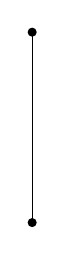
\begin{tikzpicture}[baseline={([yshift=-0.4ex]current bounding box.center)}]
      \begin{feynman}[inline=(a)]
        \vertex (a);
        \vertex (b);
        \diagram {
          a [dot] -- b [dot],
        };
        % \vertex [below=0.2em of a] {\(_{x}\)};  
        % \vertex [below=0.2em of b] {\(_{y}\)};  
      \end{feynman}
    \end{tikzpicture} = \frac{i}{2}
    \int d^Dy\, d^Dz\, J(y) \Delta(y-z) J(z) \, .
\end{equation}
Taking the functional derivatives with respect to $J$ we get a factor of two,
from acting with the first derivative on both $J(y)$ and $J(z)$:
\begin{equation}
  \label{eq:2ptOrderZeroTwo}
  G^{(2,0)}(x_1,x_2) = i \Delta(x_1-x_2)\, ,
\end{equation}
where the second index in the suffix indicates the order in the
perturbative expansion as discussed above. 

\noindent
It is easy to verify that there are no contributions to $Z[J]$ with
$E=2$ and $V=1$. 

\paragraph{V=2}

The next contributions to the two-point functions come from terms with $V=2$,
and there are two distinct connected diagram topologies at this order.
\begin{enumerate}
\item [a.] The first diagram topology that contributes to $G^{(2)}$ is
  \begin{align}
    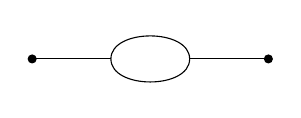
\begin{tikzpicture}[baseline={([yshift=-0.4ex]current bounding box.center)}]
      \begin{feynman}[inline=(a)]
        \vertex (a);
        \vertex (v1); 
        \vertex (v2); 
        \vertex (b);
        \diagram* {
          a [dot] -- v1 -- [out=90, in=90] v2 -- b [dot],
          v1 -- [out=-90, in=-90]  v2,
        };
      \end{feynman}
    \end{tikzpicture} = &\frac{1}{2^2} \int d^Dz_1\, d^Dz_2\, d^Dw_1\,
      d^Dw_2\, \times \nonumber \\
    &  \times J(z_1) \Delta(z_1-w_1) \Delta(w_1-w_2)^2 \Delta(w_2-z_2) J(z_2)\, .
  \end{align}
  Taking derivatives and inserting the appropriate factor of $i$
  yields a total contribution of
  \begin{align}
    G^{(2,2)}_a(x_1,x_2) = - \frac{1}{2} 
    \int d^Dw_1\, d^Dw_2\, \Delta(x_1-w_1) \Delta(w_1-w_2)^2
    \Delta(w_2-x_2)\, .
  \end{align}

\item [b.] The other contribution comes from 
  \begin{align}
    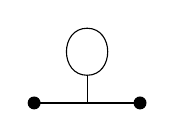
\begin{tikzpicture}[baseline={([yshift=-2.95ex]current bounding box.center)}]
      \begin{feynman}[vertical'=i to c]
        \vertex (c);
        \vertex [left=1.7em of c, dot] (a) {}; 
        \vertex [dot, right=1.7em of c](b) {};
        \vertex [above=1.0em of c](i);
%      \vertex (j);
 %     \vertex (k);
      \vertex [above=1.7em of i] (m);
      \diagram* {
%        j -- [draw=none]  i -- [draw=none] k, 
        (i) -- [half left] (m) -- [half left] (i),
%        i -- [out=155, in=25, loop, min distance=3cm] i,
        (a) -- (c) -- (b), 
        (c) -- (i), 
      };
%       \vertex [below=0.2em of a] {\(_{i_1}\)};  
%       \vertex [below=0.2em of b] {\(_{i_2}\)};  
% %      \vertex [below=0.2em of c] {\(c\)};  
%       \vertex [below=0.2em of i] {\(_{i}\)};  
    \end{feynman}
    % \begin{feynman}
    %     \vertex (v1);
    %     \vertex [left=of v1] (a); 
    %     \vertex [above=of v1] (v2); 
    %     \vertex [right=of v1] (b);
    %     \diagram* {
    %       (a) -- (v1)-- (b),
    %       (v1) -- (v2) -- [out=135, in=45, loop, min distance=3cm]  (v2),
    %     };
    %   \end{feynman}
    \end{tikzpicture} = &\frac{1}{2^2} \int d^Dz_1\, d^Dz_2\, d^Dw_1\,
      d^Dw_2\, \times \nonumber \\
    &  \times J(z_1) \Delta(z_1-w_1) \Delta(w_1-z_2) \Delta(w_1-w_2)
      \Delta(0) J(z_2)\, .
  \end{align}
  The net contribution from this diagram is
  \begin{align}
     G^{(2,2)}_b(x_1,x_2) = -\frac{1}{2} 
    \int d^Dw_1\, d^Dw_2\, \Delta(x_1-w_1) \Delta(w_1-x_2) \Delta(w_1-w_2)
      \Delta(0))\, .
  \end{align}
\end{enumerate}

\subsection{Momentum space}
\label{sec:momentum-space}

It is useful to write this correlators in momentum space. We already
discussed the representation of the free propagator in momentum space: 
\begin{align}
  \Delta(x) = \int \frac{d^Dp}{(2\pi)^D}\, e^{-ip\cdot x}
  \frac{1}{p^2 - m^2 + i\epsilon}\, .
\end{align}
The Fourier transform of the two-point correlator is defined as
\begin{align}
  \tilde{G}^{2}\left(p_1,p_2\right) 
  &= 
    \int d^Dx_1\, d^Dx_2\, e^{ip_1\cdot x_1} e^{ip_2\cdot x_2} 
    G^{(2)}(x_1,x_2) \\
  &= \int d^Dz\, d^Dx_2\, e^{ip_1\cdot z} e^{i(p_1+p_2)\cdot x_2} G^{(2)}(z) \\
  &= \left(2\pi\right)^D \delta(p_1+p_2)\, \int d^Dz\, e^{ip_1\cdot z}
    G^{(2)}(z)  \\
  &= \left(2\pi\right)^D \delta(p_1+p_2)\, \tilde{\Delta}_F(p)\, .
\end{align}
Note that translation invariance of $G^{(2)}(x_1,x_2)$ produces an overall
Dirac delta that implements conservation of the total momentum. Again
we can look at the contributions to $\tilde{G}^{(2)}(p_1,p_2)$ order by
order in perturbation theory. 

\paragraph{V=0}

At lowest order in $g$, we simply have the Fourier transform of the
free propagator:
\begin{align}
  \tilde{G}^{(2,0)}(p_1,p_2) 
  &= 
    \left(2\pi\right)^D \delta(p_1+p_2)\,
    i \tilde{\Delta}(p) \\
  &=
    \left(2\pi\right)^D \delta(p_1+p_2)\,
    \frac{i}{p_1^2-m^2+i\epsilon}\, .
\end{align}

\paragraph{V=2}

At order $g^2$, we obtain
\begin{align}
  \tilde{G}^{(2,2)}_a(p_1,p_2) 
  =& - \frac12\, \left(2\pi\right)^D \delta(p_1+p_2)\,
     \frac{1}{p_1^2-m^2+i\epsilon} \times \nonumber \\
   & \times \left\{
     \int \frac{d^D\ell}{(2\pi)^D}\, 
     \frac{1}{\ell^2-m^2+i\epsilon}
     \frac{1}{(\ell-p_1)^2-m^2+i\epsilon}
     \right\}
     \frac{1}{p_2^2-m^2+i\epsilon} \, .
\end{align}
The above expression can be represented by a Feynman diagram in
momentum space:
\begin{equation}
  \begin{tikzpicture}%[baseline=\plusheight]
    \begin{feynman}
      \vertex (a);
      \vertex [left=0.7cm of a] (i1);
      \vertex [right= of a] (b);
      \vertex [right=0.7cm of b] (f1);
      \diagram [horizontal=a to b, layered layout] {
        (i1) -- [momentum={\(p\)}] (a)
        -- [half left, momentum={[arrow shorten=0.4]\(\ell\)}] (b) 
        -- [half left, momentum={[arrow shorten=0.35]\(\ell-p\)}] (a) ,
        (f1) -- [momentum'=\(p'\)] (b)
      };
    \end{feynman}
  \end{tikzpicture}
\end{equation}
The Feynman rules in momentum space can be summarised as follows
(adapted from Srednicki's book). 
\begin{enumerate}
\item Draw $n$ lines for a $n$-point correlator. 
\item Leave one end of each external line free, and attach the other
  to the lines coming out of a vertex. 
\item The $i$-th external line carries momentum $p_i$, which we assume
  to be incoming momentum, and represent with a line pointing towards
  the vertex.
\item Four-momenta flow along the arrows, and the total momentum is
  conserved at each vertex. For a diagram without loops, this fixes
  the momentum of {\em all} internal lines. 
\item The value of the diagram is given by the product of a factor of
  $i/(p^2-m^2+i\epsilon)$ for each line with momentum $p$, a factor of
  $1/i$ for the external end of a line, and a factor $ig (1/i)^\#$ for
  each vertex, where $\#$ is the number of legs connecting at each
  vertex. 
\item A diagram with $L$ loops will have $L$ internal momenta that are
  not fixed by momentum conservation. We integrate over those momenta,
  with measure $d^p/(2\pi)^D$. 
\item Determine the symmetry factor associated to permutations of
  {\em internal} propagators and vertices. 
\end{enumerate}

\begin{Ex}
  Use the Feynman rules in momentum space to compute
  $G^{(2,2)}_b$. Check that you get the same result by performing a
  Fourier transform of the result in position space.
\end{Ex}

\section{Physical states}
\label{sec:physical-states}

The eigenstates of the Hamiltonian form a complete set of states. They
can be classified in three categories.
\begin{enumerate}
\item The vacuum state $|0\rangle$ is the lowest energy state, and
  corresponds to a state with no particles.
\item The one-particle states $|\mathbf{p},\sigma\rangle$ are
  classified by their spatial momentum. Their energy is given by the
  relativistic dispersion relation 
  \begin{equation}
    \label{eq:RelDispRel}
    E_p = \sqrt{\mathbf{p}^2 + \mphys^2}\, ,
  \end{equation}
  where $\mphys$ denotes the physical mass of the state. Note that the
  physical mass {\em does not} need to coincide with the mass that
  appears in the Lagrangian. We will discuss this point in detail
  later. Any other quantum number necessary to identify the particle
  is denoted here by $\sigma$.  The states are normalised by imposing
\begin{equation}
  \label{eq:OnePartNorm}
  \langle \mathbf{p}, \sigma | \mathbf{p}', \sigma' \rangle =
  \delta_{\sigma\sigma'}\, 
  2 E_p\, (2\pi)^{D-1} \delta(\mathbf{p}-\mathbf{p}')\, .
\end{equation}
\item The multiparticle states $|\mathbf{P};n\rangle$ are classified
  by their total spatial momentum $\mathbf{P}$, plus other parameters
  such as the relative momenta between the particles, which we denote
  collectively by $n$. The energy of the mutiparticle states is
  $\sqrt{\mathbf{P}^2+M^2}$, where $M^2$ is one of the parameters
  included in $n$. The threshold for producing multiparticle states is
  given by the energy of two particles at rest $M=2\mphys$.
\end{enumerate}
The completeness relation can be written as
\begin{align}
  |0\rangle \langle 0| 
  &+ \sum_\sigma \int d\Omega_p 
    |\mathbf{p},\sigma\rangle \langle \mathbf{p},\sigma| + \nonumber
  \\
  &+ \sum_n \int d\Omega_P 
    |\mathbf{P},n\rangle \langle \mathbf{P},n|\, = 1\, ,
\end{align}
and we have introduced the Lorentz-invariant integration measure
\begin{align}
  d\Omega_p = \frac{d^{D-1}p}{(2\pi)^{D-1}}
    \frac{1}{2E_p} \, .
\end{align}
Note that the 'sum' over $n$ is a short-hand notation, which may
involve integrations over continuum variables such as the relative
momentum, or the invariant mass of the state. 

\section{Polology}
\label{sec:polology}

In this section, we shall learn some features about the analytic
structure of field correlators, and discuss their relevance in order
to extract physical information from the correlators. Starting from an
$n$-point correlator in momentum space,
\begin{align}
  \tilde{G}^{(n)}\left(p_1, \ldots, p_n\right) 
  = \int d^Dx_1\, \ldots d^Dx_n\, 
  e^{-i p_1\cdot x_1} \ldots e^{-i p_n\cdot x_n}\, 
  \langle T\phi(x_1) \ldots \phi(x_n)\rangle\, ,
\end{align}
we want to focus on the contribution coming from the sector where the
values $x_1^0, \ldots, x_r^0$ are all larger than the values of
$x_{r+1}^0, \ldots, x_n^0$, for some value of $r$ between 1 and
$n-1$. This contribution can be written as 
\begin{align}
  \tilde{G}^{(n)}\left(p_1, \ldots, p_n\right) 
  =& \int d^Dx_1\, \ldots d^Dx_n\, 
  e^{-i p_1\cdot x_1} \ldots e^{-i p_n\cdot x_n}\, \times \nonumber \\
   &\times \theta\left(
     \min\{x_1^0 \ldots x_r^0\} - \max\{x_{r+1}^0 \ldots x_n^0\}
     \right) \nonumber \\
   &\times \langle T\Big[\phi(x_1) \ldots \phi(x_r)\Big]
     T\Big[\phi(x_{r+1}) \ldots \phi(x_n)\Big]
     \rangle\, .
\end{align}
We can introduce a complete set of states inbetween the two
$T$-ordered products, and look at the result coming from the
one-particle states. Defining new integration variables
\begin{align}
  x_i = x_1 + y_i\, , \quad \mathrm{for}\ i=2, \ldots, r\, ,
\end{align}
we can write
\begin{align}
  \phi(x_1) \ldots \phi(x_r) 
  &= \phi(x_1) \ldots \phi(x_1+y_i) \ldots \phi(x_1+y_r) \nonumber \\
  &= e^{i P\cdot x_1} \phi(0) e^{-i P\cdot x_1} \ldots e^{i P\cdot
    x_1} \phi(y_i) e^{-i P\cdot x_1} \ldots e^{i P\cdot x_1} \phi(y_r)
    e^{-i P\cdot x_1}\, ,
\end{align}
and hence
\begin{align}
  \langle 0| T \phi(x_1) \ldots \phi(x_r) | p,\sigma\rangle = 
  e^{-i p \cdot x_1}  \langle 0| T \phi(0) \ldots \phi(y_r) |
  p,\sigma\rangle\, .
\end{align}
A similar shift of the integration variables can be done using
\begin{align}
  x_i = x_{r+1} + y_i\, , \quad \mathrm{for}\ i=r+2, \ldots, n\, ,
\end{align}
The argument of the theta function can be rewritten as
\begin{align}
  \min\{x_1^0 \ldots x_r^0\} - \max\{x_{r+1}^0 \ldots x_n^0\} = 
  x_1^0 -x_{r+1}^0 + \min\{0 \ldots y_r^0\} - \max\{0 \ldots y_n^0\}\, .
\end{align}
Using the integral representation of the theta,
\begin{align}
  \theta(\tau) = -\frac{1}{2\pi i} \int_{-\infty}^{+\infty} d\omega\,
  \frac{e^{-i\omega \tau}}{\omega + i\epsilon}\, ,
\end{align}
and performing the integrals over $x_1$ and $x_{r+1}$, yields
\begin{align}
  \tilde{G}^{(n)}(p_1, \ldots, p_n) 
  &= \int d^Dy_2 \ldots d^Dy_r\, d^Dy_{r+2} \ldots d^Dy_n \, \nonumber
  \\
  & \times e^{-ip_2\cdot y_2} \ldots e^{-ip_{r}\cdot y_r} 
    \, e^{-ip_{r+2}\cdot y_{r+2}} \ldots e^{-ip_{n}\cdot y_n}
    \nonumber \\
  & \times \frac{-1}{2\pi i} \int \frac{d\omega}{\omega + i\epsilon}\, 
    \exp\left\{
    -i \omega \left[ 
    \min\{0 \ldots y_r^0\} - \max\{0 \ldots y_n^0\}
    \right]
    \right\} \nonumber \\
  & \times \sum_\sigma \int d\Omega_p
    \langle 0 |  T \phi(0) \ldots \phi(y_r) |
    p,\sigma\rangle \langle p, \sigma | T \phi(0) \ldots \phi(y_n)
    |0\rangle \nonumber \\
  & \times (2\pi)^D \delta(\mathbf{p} - \mathbf{p}_1 - \ldots -
    \mathbf{p}_r) \, 
    \delta(E_p + \omega - p_1^0 - \ldots - p_{r}^0) \nonumber \\
  & \times (2\pi)^D \delta(\mathbf{p} + \mathbf{p}_{r+1} + \ldots +
    \mathbf{p}_n) \, 
    \delta(E_p + \omega + p_{r+1}^0 + \ldots + p_{n}^0) \, .
\end{align}
Performing the integrals over the spatial components of $p$ and
$\omega$ yields
\begin{align}
  &\delta(\mathbf{p}_1+ \ldots +\mathbf{p}_n)\, \mathrm{and}\, , \nonumber \\
  & \delta(p_1^0 + \ldots + p_n^0) \frac{1}{q^0-E_p +i\epsilon}\, ,
\end{align}
respectively, where the four-momentum $q$ is defined as
\begin{align}
  q=p_1 + \ldots + p_r = -p_{r+1} - \ldots - p_n\, .
\end{align}
Finally, if we are interested in the residue at the pole, we can rewrite
\begin{align}
  \frac{1}{q^0-E_p + i\epsilon} \longrightarrow \frac{2 E_p}{q^2-\mphys^2 + i\epsilon}\, 
\end{align}
Collecting all the terms, and ignoring a phase factor that reduces to
one at the pole, we find that the one-particle state contribution to the
integration over the specific sector that we considered above yields
\begin{align}
  \tilde{G}^{(n)}(p_1,\ldots,p_n) \longrightarrow
  \delta(p_1+\ldots+p_n)\, \frac{1}{q^2-\mphys^2+i\epsilon}\, 
  \sum_\sigma M_{0|q\sigma}(p_2,\ldots,p_r) M_{q\sigma|0}(p_{r+2},
  \ldots, p_n)\, .
\end{align}
In the equation above we have defined
\begin{align}
  M_{0|q\sigma}(p_2,\ldots,p_r) 
  &= \int d^Dy_2 \ldots d^Dy_r\, 
    e^{-ip_2\cdot y_2} \ldots e^{-ip_r\cdot y_r}
    \langle 0 |  T \phi(0) \ldots \phi(y_r) |
    q,\sigma\rangle \, , \\
 M_{q\sigma|0}(p_{r+2},\ldots, p_n) 
  &= \int d^Dy_{r+2} \ldots d^Dy_n\, 
    e^{-ip_{r+2}\cdot y_{r+2}} \ldots e^{-ip_n\cdot y_n}
    \langle q,\sigma |  T \phi(0) \ldots \phi(y_n) |
    0\rangle \, ,
\end{align}
and we notice that this contribution appears multiplied by a Dirac
delta that enforces the conservation of total momentum. The important
result here is that the correlators in momentum space have a pole
singularity whenever $q=p_1+\ldots+p_r$ {\em goes on-shell}, \ie
$q^2=\mphys^2$.

Note that these results are completely general, and in particular do
not rely on the perturbative definition of the correlators. 

\section{K\"allen-Lehmann representation}
\label{sec:kall-lehm-repr}

Let us now come back to the 2-point function, and find a representation
that allows us to extract some physical information about the scalar
field. We define the full propagator as
\begin{equation}
  \label{eq:FullProp}
  \Delta_F(x-y) = i \langle 0| T \phi(x) \phi(y) |0\rangle \, ,
\end{equation}
and define the field so that
\begin{equation}
  \label{eq:FieldNorm}
  \langle 0 | \phi(x) | 0\rangle = 0\, ,\ \mathrm{and}\
  \langle \mathbf{p}| \phi(0) | 0\rangle = 1\, ,
\end{equation}
where $|\mathbf{p}\rangle$ represents the physical one-particle state,
and we have dropped the dependence on $\sigma$. As usual the full
propagator in momentum space is defined by taking the Fourier
transform:
\begin{equation}
  \label{eq:FullPropMom}
  \tilde{\Delta}_F(p) = 
  \int d^Dx\,  e^{ip\cdot(x-y)} \Delta(x-y)\, .
\end{equation}

\paragraph{Free theory}

With these conventions, the free theory result for the propagator is
\begin{equation}
  \label{eq:FreePropAgain}
  \tilde\Delta(p) = \frac{1}{p^2-m^2+i\epsilon}\, .
\end{equation}
Eq.~(\ref{eq:FreePropAgain}) shows that $\tilde{\Delta}$ has a pole at
$p^2=m^2$. For the free particle we find a pole in the propagator,
at a value which coincides with the parameter in the Lagrangian.

\paragraph{Interacting theory}

For the interacting theory, we can derive a general expression, which
again does not rely on the perturbative definition of the two-point
function. Let us first consider the case where $x^0>y^0$:
\begin{align}
  \langle 0| T \phi(x) \phi(y) |0\rangle
  =& \langle 0| \phi(x) \phi(y) |0\rangle \nonumber \\
  =& \langle 0| \phi(x) |0\rangle \langle 0 | \phi(y) |0\rangle +
     \nonumber \\
  &+ \int d\Omega_p\, \langle 0| \phi(x)| \mathbf{p}\rangle
    \langle \mathbf{p} | \phi(y) |0\rangle + \nonumber \\
  &+ \sum_n \int d\Omega_P\, \langle 0| \phi(x) |\mathbf{P}, n\rangle
    \langle \mathbf{P}, n |\phi(y) |0\rangle\, .
\end{align}
The conventions in Eq.~(\ref{eq:FieldNorm}) allow us to simplify the
expression above.
\begin{align}
  \langle 0| T \phi(x) \phi(y) |0\rangle
  =& \int d\Omega_p\, e^{-ip\cdot (x-y)} + \nonumber \\
   &+ \sum_n \int d\Omega_p\, e^{-ip\cdot (x-y)}\, \left|
    \langle \mathbf{p}, n |\phi(0) |0\rangle \right|^2 \, .
\end{align}
Because we are working with a scalar field, the matrix element
$\langle \mathbf{p}, n |\phi(0) |0\rangle$ is invariant under Lorentz
transformations, and therefore can only depend on $p$ via the
invariant mass $M^2$. We can therefore introduce the {\em spectral
  density}
\begin{align}
  \label{eq:SpecDen}
  \rho(s) = \sum_n \left|
    \langle \mathbf{p}, n |\phi(0) |0\rangle \right|^2 \, 
  \delta(s-M^2)\, ,
\end{align}
and write the two-point correlator as
\begin{align}
  \langle 0| T \phi(x) \phi(y) |0\rangle
  =& \int d\Omega_p\, e^{-ip\cdot (x-y)} + \nonumber \\
   &+ \int_{4m^2}^\infty ds\, \rho(s) \int d\Omega_p\,  e^{-ip\cdot
     (x-y)}\, .
\end{align}
Similar manipulations for the case $y^0>x^0$ yield
\begin{align}
  \langle 0| T \phi(x) \phi(y) |0\rangle
  =& \int d\Omega_p\, e^{ip\cdot (x-y)} + \nonumber \\
   &+ \int_{4m^2}^\infty ds\, \rho(s) \int d\Omega_p\,  e^{ip\cdot
     (x-y)}\, .
\end{align}
Collecting both contributions to the $T$-ordered product 
\begin{align}
  \langle 0| T \phi(x) \phi(y) |0\rangle
  = \theta(x^0-y^0)  \langle 0| \phi(x) \phi(y) |0\rangle
  + \theta(y^0-x^0)  \langle 0| \phi(y) \phi(x) |0\rangle\, ,
\end{align}
and using 
\begin{align}
  \frac{1}{i} \int \frac{d^Dp}{(2\pi)^D}\,
  \frac{e^{-ip\cdot(x-y)}}{p^2-\mphys^2+i\epsilon} = 
  \theta(x^0-y^0) \int d\Omega_p\, e^{-ip\cdot(x-y)} +
  \theta(y^0-x^0) \int d\Omega_p\, e^{ip\cdot(x-y)}\, , 
\end{align}
we finally obtain
\begin{align}
  \langle 0| T \phi(x) \phi(y) |0\rangle
  =& \int \frac{d^Dp}{(2\pi)^D}\,
     e^{-ip\cdot(x-y)} \Big[
     \frac{1}{p^2-\mphys^2+i\epsilon} + \nonumber \\
  \label{eq:KLFourier}
  & + \int_{4\mphys^2}^\infty ds\, \rho(s) \frac{1}{p^2-s+i\epsilon} 
     \Big]\, .
\end{align}
Eq.~(\ref{eq:KLFourier}) allows us to read the expression for the full
propagator in momentum space:
\begin{align}
  \label{eq:KLusual}
  \tilde{\Delta}_F(p) = \frac{1}{p^2-\mphys^2+i\epsilon} 
  + \int_{4\mphys^2}^\infty ds\, \rho(s) \frac{1}{p^2-s+i\epsilon}\, . 
\end{align}
We see that the two-point correlator of a field $\phi$ that satisfies
the conditions in Eq.~(\ref{eq:FieldNorm}) has a pole for
$p^2=\mphys^2$, with residue exactly equal to one. Note that the field
$\phi$ does not need to be the field that appears in the
Lagrangian. Knowledge about the multiparticle states of the theory is
encoded in the two-point function via the integral on the RHS side of
Eq.~(\ref{eq:KLusual}). 

\section{S Matrix}
\label{sec:s-matrix}

In order to compute the quantum amplitude for a physical process
involving arbitrary numbers of particles in the initial and final
state, we need to compute the overlap of a state prepared in the
distant past (the so-called {\em in} state), with the resulting final
state in the distant future (the so-called {\em out} state). If
we want to describe a $2\to n$ process -- like a $pp$ collision at
the LHC -- we need to compute
\begin{equation}
  \label{eq:ScattAmpl}
  \langle \mathbf{p}_1, \ldots, \mathbf{p}_n; \mathrm{out} |
  \mathbf{k}_1, \mathbf{k}_2; \mathrm{in}\rangle\, .
\end{equation}
The $S$-matrix allows us to express this scalar product between in-
and out-states in terms of states defined at any common reference
time: 
\begin{equation}
  \label{eq:SMatDef}
   \langle \mathbf{p}_1, \ldots, \mathbf{p}_n; \mathrm{out} |
  \mathbf{k}_1, \mathbf{k}_2; \mathrm{in}\rangle = 
   \langle \mathbf{p}_1, \ldots, \mathbf{p}_n | S |
  \mathbf{k}_1, \mathbf{k}_2\rangle\, .
\end{equation}
It is usual to separate the $S$ matrix into the identity operator,
corresponding to particles not interacting, plus a non-trivial part
which is usually denoted $T$:
\begin{equation}
  \label{eq:TMatDef}
  S = 1 + i T\, .
\end{equation}

\section{LSZ reduction}
\label{sec:lsz-reduction}

An important corollary of the result shown in
section~\ref{sec:polology} is obtained by setting $r=1$. In this case,
the previous discussion allows us to conclude that the correlators in
momentum space have a pole whenever the momentum of one of the fields
is on-shell. Therefore an $n$-point correlation function has (at
least) $n$ poles, each corresponding to one of the momenta
$p_i\to \mphys^2$. The residue at this multiple pole yields the $S$-matrix
for a scattering process involving $n$-particles:
\begin{align}
   \langle p_{1}' \ldots p_{m'}'; \mathrm{out} | p_{1} \ldots p_{m};
  \mathrm{in} \rangle 
  =& 
  \langle p_{1}' \ldots p_{m'}' | S | p_{1} \ldots p_{m} \rangle \\
  =& 
  \lim_{p_j^2,p_k'^2 \to \mphys^2} \prod_{k=1}^{m'}
  (p_k'^2-\mphys^2+i\epsilon)
  \prod_{j=1}^{m}
  (p_j^2-\mphys^2+i\epsilon) \, \nonumber \\
  & \times 
    \tilde{G}^{(m+m')}(p_1, \ldots, p_{m}, -p_1', \ldots, -p_{m'}')\, ,
\end{align}
where $n=m+m'$, and the fields are normalised so that
\begin{align}
  \langle \mathbf{p} | \phi(0) | 0\rangle = 1\,.
\end{align}
We will return to the question of the normalisation of the field
later. The LSZ reduction formula provides an elegant way to represent
quantum amplitudes using Feynman diagrams in momentum space. We adopt
the same rules discussed above, with the following modifications.
\begin{enumerate}
\item We associate an outgoing momentum to the external lines that
  correspond to particles in the final state. 
\item We multiply each external line by a factor of
  $-i(p^2-\mphys^2+i\epsilon)$ -- the correlators multiplied by these
  factors are called {\em truncated} (or {\em amputated}) correlators.
\end{enumerate}

A heuristic derivation of the LSZ reduction formula is discussed in
Problem Sheet 4.

\begin{Ex}
  Compute the amplitude for the scattering process
  \[
    p_1 p_2 \longrightarrow p_1' p_2'
  \]
  at order $g^2$ in the $\phi^3$ scalar theory. You can assume that
  $\mphys=m$ in this calculation.
\end{Ex}

\section{Optical Theorem}
\label{sec:optical-theorem}

Physical constraints translate into relations between correlators. It
is important to be able to derive these relations, and to understand
their physical content. One example is provided by the unitarity of
the $S$-matrix, \ie by the conservation of probability in quantum
mechanics. Unitarity is written as
\begin{equation}
  \label{eq:SmatUnit}
  S^\dagger S = 1\, .
\end{equation}
Inserting the representation of $S$ in terms of the transition matrix
yields
\begin{equation}
  \label{eq:TmaUnit}
  -i \left(T - T^\dagger\right) = T^\dagger T\, .
\end{equation}
Let us consider the matrix element of Eq.~(\ref{eq:TmaUnit}) between an
initial state $a$ and a final state $b$, and let us factor out a Dirac
delta that corresponds to total momentum conservation, 
\begin{equation}
  \label{eq:MAmplitude}
  \langle b | T | a\rangle = (2\pi)^D \delta(P_a - P_b)\, \mathcal{M}(a
  \to b)\, .
\end{equation}
Some simple algebra yields on the LHS
\begin{equation}
  \label{eq:MLHS}
  -i (2\pi)^D \delta\left(P_a-P_b\right) \left[
    \mathcal{M}(a\to b) - \mathcal{M}(b \to a)^*
    \right]\, . 
\end{equation}
On the RHS we can insert a complete set of states, and rewrite it as
\begin{equation}
  \label{eq:MRHS}
   (2\pi)^D \delta\left(P_a-P_b\right) \sum_f \int d\Omega_f\,
   (2\pi)^D \delta\left(P_a-P_f\right) \mathcal{M}(b\to f)^*
   \mathcal{M}(a\to f)\, .
 \end{equation}
The unitarity condition simplifies for $a=b$, 
\begin{equation}
  \label{eq:OptThm}
  2 \mathrm{Im}\ \mathcal{M}(a\to a) = 
  \sum_f \int d\Omega_f  (2\pi)^D \delta\left(P_a-P_f\right) 
  \left|
    \mathcal{M}(a\to f)
  \right|^2\, .
\end{equation}
This is the so-called {\em optical theorem}, which relates the
imaginary part of the forward $a\to a$ amplitude (LHS) to the total cross
section $a\to f$ (RHS), summed over {\em all} final states $f$.

\section{Ward identities}
\label{sec:ward-identities}

The final example of relations between correlators that we are going
to discuss are the so-called {\em Ward identities}. Ward identities
are equalities between field correlators that are obtained as a
consequence of symmetries of the system. In classical mechanics,
symmetries of the action translate into conserved currents according
to Noether's theorem. As we will show in this section, the analogue of
current conservation in quantum field theory is precisely the Ward
identity. 

In order to derive the identities, let us start by considering a
symmetry transformation of the field, \ie a transformation
\begin{equation}
  \label{eq:FieldTrans}
  \phi(x) \mapsto \phi'(x)=\phi(x) + \epsilon \delta\phi(x) \, ,
\end{equation}
such that for constant $\epsilon$ the action is unchanged. If we introduce
a dependence on the space-time coordinate, $\epsilon(x)$, then the
variation of the action can be written
\begin{align}
  \label{eq:SVar}
  \delta S &= \int d^Dx\, \frac{\delta S}{\delta\phi(x)} \epsilon(x)
             \delta\phi(x) \\
             &= -\int d^Dx\, \epsilon(x) \partial_\mu j^\mu(x)\, , 
\end{align}
where $j^\mu(x)$ is precisely the Noether current that is conserved in
the classical theory. 

In order to derive the Ward identities, we use
Eq.~(\ref{eq:FieldTrans}) to perform a change of integration variables
in the functional integral
\begin{equation}
  \label{eq:ChangeOfVars}
  \int \mathcal{D}\phi\, e^{iS[\phi]} O(\phi) = 
  \int \mathcal{D}\phi'\, e^{iS[\phi']} O(\phi') \, ,
\end{equation}
and then expand the RHS to first order in $\epsilon$:
\begin{align}
  \int \mathcal{D}\phi\, e^{iS[\phi]} O(\phi) 
  =& \int \mathcal{D}\phi\, e^{iS[\phi]}\, 
     \left[
     1 + i \delta S[\phi]
     \right]\, 
     \left[
     O(\phi) + \delta O
     \right]
     \, ,
\end{align}
where $O$ is a generic function of the field $\phi$. We can now
substitute the expressions for $\delta S$ and $\delta O$:
\begin{align}
  \int \mathcal{D}\phi\, e^{iS[\phi]} \left\{
  -i \int d^Dx\, \epsilon(x) \partial_\mu j^\mu(x)
  O(\phi) + \int d^Dx\, \frac{\delta O(\phi)}{\delta\phi(x)} \epsilon(x)
  \delta \phi(x)
  \right\} = 0\, .
\end{align}
Rearranging the terms above allows us to write the identity in a way
that makes its physical content more obvious: 
\begin{align}
  \label{eq:IntWardId}
  \int d^Dx\, \epsilon(x) \left\{
  -i \langle \partial_\mu j^\mu(x)
  O(\phi) \rangle +  
  \langle \frac{\delta O(\phi)}{\delta\phi(x)}
  \delta \phi(x) \rangle \right\} = 0\, .
\end{align}
Eq.~(\ref{eq:IntWardId}) is sometimes referred to as an {\em
  integrated Ward identity}. Since it has to be satisfied for every
function $\epsilon(x)$, we can derive the {\em Ward identity}:
\begin{align}
  \label{eq:WardId}
   -i \langle \partial_\mu j^\mu(x)
  O(\phi) \rangle +  
  \langle \frac{\delta O(\phi)}{\delta\phi(x)}
  \delta \phi(x) \rangle = 0\, .
\end{align}
There are two important physical results encoded in Eq.~(\ref{eq:WardId}).
\begin{enumerate}
\item Symmetry in QFT translates into a relation between
  correlators. This is true beyond perturbation theory and is used in
  defining the renormalization conditions in QFT.
\item Current conservation in QFT is realised at the level of the
  insertion of $\partial_\mu j^\mu(x)$ in field correlators, up to
  the terms that come from the variation of $O$. If $O$ is a product
  of local fields, this variations is localised in space-time, \ie the
  contributions are all proportional to Dirac deltas. These terms are
  called {\em contact terms}.  
\end{enumerate}

Note that in deriving the Ward identity above we have assumed that the
integration measure $\mathcal{D}\phi$ is invariant, \ie
$\mathcal{D}\phi=\mathcal{D}\phi'$. There are examples where the
measure is {\em not} invariant, which lead to extra terms in the Ward
identities. In these cases the Ward identities are called {\em
  anomalous}. 


\chapter{Dynamics - General Aspects}
\label{cha:prop-corrs}
\newcommand{\Hin}{\mathcal{H}_{\mathrm{in}}}
\newcommand{\matH}{\mathcal{H}}
\newcommand{\Dspace}{\scriptscriptstyle{D-1}}
\newcommand{\Dall}{\scriptscriptstyle{D}}
\newcommand{\instate}{\mathrm{in}}
\newcommand{\outstate}{\mathrm{out}}
\newcommand{\dddt}{\frac{\overleftrightarrow{\partial}}{\partial t}}

\section{Time Evolution Pictures in Quantum Mechanics}
\label{sec:reps-quant}

In order to set the notation, we briefly summarise the different representations
used to describe the time evolution of quantum systems. The state of the system
at $t=0$ is described by a vector $\ket{\psi} \in \mathcal{H}$, where
$\mathcal{H}$ is the Hilbert space of physical states.

\paragraph{Schr\"odinger Picture}

In the Schr\"odinger representation the time evolution is encoded in the time
dependence of the state vector, $\ket{\psi_S(t)}$, which evolves according to
the Schr\"odinger equation
\begin{equation}
    \label{eq:SchrodEq}
    i \partial_t \ket{\psi_S(t)} = H \ket{\psi_S(t)}\, ,
\end{equation}
where $H$ is the Hamiltonian operator for the system under study. The state of
the system at time $t$ is 
\begin{equation}
    \label{eq:SchrTimeEvol}
    \ket{\psi_S(t)} = e^{-i H t} \ket{\psi}\, .
\end{equation}
Operators
associated to observables, $O_S$, are time independent (unless the observable
itself has an explicit dependence on time). The expectation value of the
observable at time $t$ is 
\begin{equation}
    \label{eq:SchrodExp}
    O(t) = \langle \psi_S(t) | O_S | \psi_S(t) \rangle\, .
\end{equation}

\paragraph{Heisenberg Picture}

In the Heisenberg representation, the state vector does not evolve in time. At
all times $t$, $\ket{\psi_H(t)}=\ket{\psi}$. We will therefore drop the suffix
$H$ when we refer to states in the Heisenberg representation. Time evolution is
encoded in the time dependence of the operators $O_H(t)$. Clearly the
expectation value at time $t$ should not depend on whether we work in the
Schr\"odinger or Heisenberg representation:
\begin{equation}
    \label{eq:HeisenExp}
    O(t) = \langle \psi | O_H(t) | \psi \rangle\, .
\end{equation}
Comparing Eqs.~\eqref{eq:SchrodExp} and~\eqref{eq:HeisenExp} we deduce that
\begin{equation}
    \label{eq:HeisenOp}
    O_H(t) = e^{iHt} O_S e^{-iHt}\, ,
\end{equation}
and therefore 
\begin{equation}
    \label{eq:HeisenEvol}
    i \frac{d}{dt} O_H(t) = - \left[H, O_H(t)\right]\, ,
\end{equation}
where $H$ is the Hamiltonian again.~\footnote{Clearly, the Hamiltonian operator
in the Heisenberg representation is time-independent. Do not confuse the
Hamiltonian $H$ and the suffix $H$, used to denote the Heisenberg
representation.}

\paragraph{Interaction Picture}

The interaction picture interpolates between the previous two. In this case the
Hamiltonian is divided into a {\it free} Hamiltonian $H_0$ and an interaction
term $V$. The time dependent state vector in the interaction picture is defined
by `subtracting' the free evolution from the Schr\"odinger state vector at time
$t$:
\begin{equation}
    \label{eq:IntPictEvol}
    \ket{\psi_{\mathrm{int}}(t)} = e^{i H_0 t} \ket{\psi_S(t)}\, .
\end{equation}
The operators are also time-dependent:
\begin{equation}
    \label{eq:IntPictOps}
    O_{\mathrm{int}}(t) = e^{i H_0 t} O_S e^{-i H_0 t}\, .
\end{equation}
In this representation the free Hamiltonian is time independent,
\begin{equation}
    \label{eq:H0IntPict}
    H_{0,\mathrm{int}}(t) = H_0\, ,
\end{equation}
and the time evolution of the states is described by a first-order differential
equation similar to Schr\"odinger's equation, where $V_{\mathrm{int}}$ replaces $H$,
\begin{equation}
    \label{eq:IntPictEvolEq}
    i \partial_t \ket{\psi_{\mathrm{int}}(t)} = V_{\mathrm{int}}(t) \,
    \ket{\psi_{\mathrm{int}}(t)}\, .
\end{equation}

\paragraph{Fields} Note that fields in QFT are treated as operator-valued 
distributions and therefore
\begin{equation}
    \label{eq:HvIntFields}
    \phi_H(t,\mathbf{x}) = U(t)^\dagger \phi_{\mathrm{int}}(t,\mathbf{x}) 
    U(t)\, ,
\end{equation}
where
\begin{equation}
    \label{eq:Uoperator}
    U(t) = e^{iH_0t} e^{-iHt}\, .
\end{equation}

\paragraph{Conventions for Generators of Translations}

Using a $D$-dimensional covariant notation, and a Minkovski metric 
\begin{equation}
    \label{eq:MostlyMinus}
    \eta_{\mu\nu} = \mathrm{diag}\left\{1, -1, -1, \ldots \right\}\, ,
\end{equation}
we represent the $D$-dimensional momentum operator in position space as
\begin{equation}
    \label{eq:MomOp}
    P^\mu = i \partial^\mu\, ,
\end{equation}
which reduces to the usual expressions for the Hamiltonian $P^0$ and the spatial
components of the momentum $P^k$. The momentum being the generator of
translations, the wave function of a system in the Schr\"odinger picture obeys
\begin{equation}
    \label{eq:PsiTranslation}
    \psi\left(x+a\right) = e^{-i P\cdot a} \psi\left(x\right)\, ,
\end{equation}
while for the field operators in the Heisenberg representation
\begin{equation}
    \label{eq:PhiTranslation}
    \phi_H(x+a) = e^{i P\cdot a} \phi_H(x) e^{-i P\cdot a}\, .
\end{equation}

\section{Asymptotic States}
\label{sec:AsymptStates}

`In' and `Out' states are states of the interacting theory in the Heisenberg
representation, which are characterized by the behaviour of the system in the
far past and the far future respectively, where the particles can be considered
to be well separated. The separation between particles implies that these states
should be in a one-to-one correspondence with free-particle states. Let us focus
here on in-states, similar results hold for the out-states. The Hilbert space of
in-states is denoted $\Hin$. A basis of $\Hin$ is made of simultaneous momentum
eigenstates of $N$ particles, where $N$ spans the set of integer numbers
\begin{equation}
    \label{eq:HinBasis}
    \left\{ \ket{k_1 \ldots k_N; \mathrm{in}}, N \in \mathbb{N} \right\}\, .
\end{equation}
Clearly the individual momenta are not conserved quantities, while translation
invariance guarantees that the total momentum $P^\mu$ is conserved,
\begin{equation}
    \label{eq:TotMomConserv}
    P^\mu \ket{k_1 \ldots k_N; \mathrm{in}} = 
    \left(\sum_{m=1}^N k^\mu_m\right) 
    \ket{k_1 \ldots k_N; \mathrm{in}}\, .
\end{equation}
From the definitions summarised in Sec.~\ref{sec:reps-quant}, we see that states
in the Schr\"odinger and Heisenberg pictures coincide at $t=0$. We can express
the fact that in-states behave like free-particle states as $T \to -\infty$. Let
$\ket{a; 0}$ be a free-particle state, we require
\begin{equation}
    \label{eq:InAsympOne}
    \lim_{T\to-\infty} e^{-i H_0 T} \ket{a;0} =
    \lim_{T\to-\infty} e^{-i H T} \ket{a; \mathrm{in}}\, ,
\end{equation}
which we rewrite as~\footnote{There is potential for sloppiness here, but I
don't think it does matter.}
\begin{align}
    \label{eq:InAsympTwo}
    \ket{a; \mathrm{in}} &= \lim_{T\to-\infty} e^{i H T} e^{-i H_0 T} \ket{a;0}
    \\
    \label{eq:MollerOne}
    &= \Omega^+ \ket{a; 0}\, .
\end{align}
Similarly for out-states,
\begin{align}
    \label{eq:OutAsympTwo}
    \ket{a; \mathrm{out}} &= \lim_{T\to +\infty} e^{i H T} e^{-i H_0 T} \ket{a;0}
    \\
    \label{eq:MollerTwo}
    &= \Omega^- \ket{a; 0}\, .
\end{align}
Finally we recall the definition of the $S$ matrix: 
\begin{align}
    \label{eq:SMatOne}
    S_{ab} &= \langle a; \mathrm{out} | b; \mathrm{in} \rangle \\
    \label{eq:SMatTwo}
    &= \langle a; 0 | \left(\Omega^-\right)^\dagger
    \Omega^+ | b; 0\rangle\, .
\end{align}

\section{Axiomatic Field Theory - States and Fields}
\label{sec:AFTONe}

We work with fields in the Heisenberg picture, denoted $\phi(x)$. The axioms
needed to build a quanutm theory of fields can be divided into three main
categories: axioms that specify the states of the theory, axioms that establish
the properties of fields, and axioms that define the field-particle duality. In
this section we look at the first two categories, while deferring the discussion
of field-particle duality to a later section. 

\paragraph{State Axioms.}

The structure of the Hilbert space of quantum states, $\mathcal{H}$, is defined
by the following axioms. 

\begin{enumerate}
    \item [{\bf Ia.}] $\mathcal{H}$ is a separable~\footnote{
        A separable space contains a countable, dense subset. For now, we are not 
        going to pay too much attention to the places where this property is used. 
    } Hilbert space, which carries
    a unitary representation $U(\Lambda,a)$ of the Poincar\'e group, 
    \begin{equation}
        \label{eq:PoincaRep}
        \ket{\alpha} \in \matH\, , \quad U(\Lambda,a) \ket{\alpha} \in \matH\, .
    \end{equation}
    
    \item [{\bf Ib.}] The spectrum of $P^\mu$ lies in the forward light-cone,
    \begin{equation}
        \label{eq:ForwSpec}
        P^0 \geq 0\, , \quad P^2 \geq m^2\, ,
    \end{equation}
    where $m$ is the mass of the single-particle state. 

    \item [{\bf Ic.}] There is a unique vacuum state $\ket{0}$, normalized such that $\langle 0 | 0\rangle = 1$. Note that this assumption implies the absence of spontaneous symmetry breaking. 
    
    \item [{\bf Id.}] Existence of a mass gap, the spectrum of $P^2$ is empty between 0 and $m^2$.
\end{enumerate}

\paragraph{Field Axioms.}

This set of axioms specifies the properties of quantum fields and their
expectation values. Details of the theory of distributions are summarised 
in Chapter~\ref{chap:distr-notes}.

\begin{enumerate}
    \item [{\bf IIa.}] The Heisenberg fields $\phi(x)$ are operator-valued distributions, \ie
    \begin{equation}
        \label{eq:OpValuedDistr}
        \forall f \in \mathcal{S}(\mathbb{R}^D)\, , 
        \phi_f = \int d^Dx\, f(x) \phi(x)
    \end{equation}
    is an unbounded operator on $D \subset \matH$,~\footnote{
        Here we use $D$ to denote a dense set, {\em not} the number of 
        spacetime dimensions. Hopefully the meaning of the symbol is clear
        from the context. 
    } where $D$ is dense in $\matH$
    and $\mathcal{S}$ is the set of Schwartz test functions. The image of $D$ is
    a subset of $D$ itself, which allows to perform subsequent applications of
    the smeared operators, \eg
    \begin{align}
        \langle 0 | \phi_{f_1} \ldots \phi_{f_n} | 0\rangle 
        &= \int d^Dx_1 \ldots d^Dx_n\, f_1(x_1) \ldots f_n(x_n) \, 
        W(x_1 \ldots x_n) \, , \\
        W(x_1 \ldots x_n)
        &= \langle 0 | \phi(x_1) \ldots \phi(x_n) | 0\rangle\, .
    \end{align} 
    The correlators $W(x_1 \ldots x_n)$ are called {\em Wightman functions}. The
    Wightman functions are {\em tempered}\ distributions, \ie
    \begin{equation}
        \label{eq:TempDistr}
        W(z) = D^m F(z)\, , \quad F(z) < C (1 + |z_E|^2)^p\, ,
    \end{equation}
    for some integer values of $p$. Note that $z$ is a generalized coordinate
    that collects $x_1, \ldots x_n$, $m=(m_1 \ldots m_n)$ is a vector of
    integers, $D^m$ is a short-hand for 
    \begin{equation}
        \label{eq:MultiDeriv}
        D^m = 
        \frac{\partial^{|m|}}{\partial x_1^{m_1} \partial x_2^{m_2} \ldots}\, ,
    \end{equation}
    and $|m| = m_1 + \ldots + m_n$.

    \item [{\bf IIb.}] Under Poincar\'e transformations $\left\{\Lambda, a\right\}$
    \begin{align}
        & U(\Lambda,a)\, \phi_f\, U(\Lambda,a)^\dagger 
            = \phi_{f_{\Lambda,a}} \, , \\
        & f_{\Lambda,a}(x) = f\left(\Lambda^{-1}(x-a)\right)\, .
    \end{align}

    \item [{\bf IIc.}] If $f_1$ and $f_2$ have compact supports $V_1$ and $V_2$ respectively, and if 
    \[
        \forall x_1 \in V_1\, , \forall x_2 \in V_2 \, ,    
        \quad (x_1 - x_2)^2 < 0\, ,
    \]
    then 
    \begin{equation}
        \label{eq:SmearedLightConeComm}
        \left[ \phi_{f_1} , \phi_{f_2} \right] = 0\, .
    \end{equation}

    \item [{\bf IId.}] Polynomials of $\phi_f$, with all possible choices of $f$, 
    acting on $\ket{0}$ form a dense set in $\matH$.
\end{enumerate}

Because of translation invariance, the Wightman functions only depend on $n-1$
variables
\begin{equation}
    \label{eq:WightFunTransInv}
    W(x_1 \ldots x_n) = \mathcal{W}\left(\xi_1 \ldots \xi_{n-1}\right)\, ,
\end{equation}
where $\xi_i = x_i - x_{i+1}$. They can be extended by
analytical continuation to the tube $\mathcal{T}_n$, as discussed in Chapter~\ref{chap:distr-notes}, 
$\zeta_i = \xi_i - i \eta_i$, with $\eta_i^2>0$.
The latter functions are invariant under complex Lorentz transformations
\begin{equation}
    \label{eq:ComplexLorentzInv}
    \mathcal{W}(\Lambda\zeta_1 \ldots \Lambda\zeta_{n-1}) =
    \mathcal{W}(\zeta_1 \ldots \zeta_{n-1})\, ,
\end{equation}
which in turn implies that $\mathcal{W}$ is an analytical function of the scalar
products $\zeta_i \cdot \zeta_j$. Note that the Euclidean {\em Schwinger
functions}\ are defined by analytical continuation~\footnote{In Euclidean space 
the spacetime vectors $x_E$ have $D$ components that are related to the Minkowski 
ones as follows
\[
 x_E^i = x^i\, ,~\mathrm{for}~i=1, \ldots,D-1\, , \quad x_E^D = i x^0\, .   
\] }
\begin{equation}
    \label{eq:SchwingFunDef}
    S(x_1 \ldots x_n) = 
        W\left((-i x_1^D, \mathbf{x}_1) 
        \ldots (-i x_n^D, \mathbf{x}_n)\right)\, .
\end{equation}

We can define an $x$-dependent smeared field
\begin{align}
    \label{eq:XdepPhiSmeared}
    \phi_f(x) 
    &= e^{i P \cdot x} \phi_f e^{-i P \cdot x} \\
    &= \int d^Dz\, f(z-x) \phi(z)\, ,
\end{align}
and bilocal smeared operators
\begin{equation}
    \label{eq:BilocalSmeared}
    \phi_f = \int d^Dx_1 d^Dx_2\, f\left(x_1 - x_2\right) 
    \phi(x_1) \phi(x_2)\, .
\end{equation}
The Fourier transform of a local smeared operator
\begin{equation}
    \label{eq:FourierSmeared}
    \tilde\phi_f(p) = \int d^Dx\, e^{i p\cdot x} \phi_f(x)
\end{equation}
carries exactly momentum $p$. The smearing of the field in position space does
not affect the momentum of the Fourier transform, and hence
\begin{equation}
    \label{eq:DeltaMomSmeared}
    \langle \alpha | \tilde\phi_p(p) | \beta\rangle 
    \propto \delta\left(P_\alpha-P_\beta-p\right)\, .
\end{equation}

\subsection{An Example Proof: Space-like Commutation}
\label{sec:ExampleProof}

In order to develop some familiarity with the concepts we introduce above, it is
interesting to work out explicitly the proof of the following property. Let
$a=\left(0, \mathbf{a}\right)$, then axiom {\bf IIc} implies
\begin{equation}
    \label{eq:FasterThanPoly}
    \left| \langle 0 |
        \left[ \phi_{f_1}(-a), \phi_{f_2}(a)\right]
        | 0 \rangle 
    \right| < C \left|\mathbf{a}\right|^{-N}\, , \quad \forall N\, , 
    \mathrm{for}~\left|\mathbf{a}\right|\to\infty\, .
\end{equation}

\paragraph{Proof}

The expectation value in \eqref{eq:FasterThanPoly} can be written as
\begin{align}
    \label{eq:ExpComm}
    \langle 0 |
        \left[ \phi_{f_1}(-a), \phi_{f_2}(a)\right]
        | 0 \rangle =
        \int d^Dx_1 d^Dx_2\, f_1(x_1) f_2(x_2)\,
        \langle 0 | 
        \left[\phi(x_1-a), \phi(x_2+a)\right]
        | 0 \rangle\, .
\end{align}
Introducing $2D$-dimensional vectors $z=(x_1,x_2)$ and $\alpha=(a,-a)$, we define 
$F(z) = f_1(x_1) f_2(x_2)$, which is a fast-decreasing function of $z$, and
\begin{align}
    \label{eq:CommZvar}
    \langle 0 | 
        \left[\phi(x_1-a), \phi(x_2+a)\right]
        | 0 \rangle 
        &= W\left(x_1-a,x_2+a\right) - W\left(x_2+a,x_1-a\right) \\
        &= W\left(z-\alpha\right)\, .
\end{align} 
We can then rewrite
\begin{equation}
    \label{eq:SmearedCorrZvar}
    \langle 0 |
        \left[ \phi_{f_1}(-a), \phi_{f_2}(a)\right]
        | 0 \rangle 
        = \int dz\, F(z) W(z-\alpha)\, ,
\end{equation}
where $W(z)$ is a tempered distribution, 
\begin{align}
    \label{eq:WTempDist}
    W(z) &= D^m \mathcal{P}(z)\, , \\
    \mathcal{P}(z) &= c_1 \left(1 + |z|_E^2\right)^p\, , \quad \mathrm{for\ all\ } p\, .
\end{align}
If $|z|_E<|\mathbf{a}|$ then the separation between $(x_1-a)$ and $(x_2+a)$ is space-like 
and $W(z-\alpha)$ vanishes, hence, after integrating by parts, 
\begin{equation}
    \label{eq:CutIntegralW}
    \left|\langle 0 |
        \left[ \phi_{f_1}(-a), \phi_{f_2}(a)\right]
        | 0 \rangle \right| = \int_{|z|_E>|\mathbf{a}|}
        dz\, \mathcal{P}(z-\alpha)\, D^mF(z)\, .
\end{equation}
Because $W$ is a tempered distribution, we know that 
\begin{equation}
    \label{eq:PFastDecrease}
    \mathcal{P}(z-\alpha) < c_1 \left(1 + |z-\alpha|_E\right)^p 
    < c_1 \left(1 + |z|_E\right)^p  \left(1 + |\alpha|_E\right)^p \, ,
\end{equation}
for all values of $p$. The smearing functions are also fast decreasing, therefore for 
any value of $N$, 
\begin{equation}
    \label{eq:SmearFastDecrease}
    \left| D^m F(z)\right| < c_2 \left|z\right|_E^{-(N+2p+2D)}\, \left(1 + |z|_E^2\right)^p \, ,
\end{equation}
where $p$ is the same power that appears in \eqref{eq:PFastDecrease}. Finally, in spherical coordinates, 
we have that 
\[
    d^Dz = S_{2D}\, |z|_E^{2D-1} d|z|_E\, .   
\]
Putting everything together and performing the integral over $z$ outside the sphere of radius 
$|\mathbf{a}|$ yields
\begin{equation}
    \label{eq:BoundOnSmearCorr}
    \left|\langle 0 |
        \left[ \phi_{f_1}(-a), \phi_{f_2}(a)\right]
        | 0 \rangle \right| < 
        c_1 c_2 \frac{S_{2D}}{N+2p} \left(1 + 2 |\mathbf{a}|\right)^p
        |\mathbf{a}|^{-N-2p}\, , 
\end{equation}
which shows explicitly the fast decay of the correlator as a function of the distance $|\mathbf{a}|$.

\section{Ruelle Clustering Theorem}
\label{sec:RuelleClust}

Connected correlators of smeared fields can be defined in the usual way:
\begin{align}
    &\langle 0 | \phi_{f_1}(x_1) | 0 \rangle_c 
        = \langle 0 | \phi_{f_1}(x_1) | 0 \rangle \, , \\
    &\langle 0 | \phi_{f_1}(x_1) \phi_{f_2}(x_2) | 0 \rangle_c 
        = \langle 0 | \phi_{f_1}(x_1) \phi_{f_2}(x_2) | 0 \rangle -
           \langle 0 | \phi_{f_1}(x_1) | 0 \rangle \langle 0 | \phi_{f_2}(x_2) | 0 \rangle\, , \\
    &\ldots \nonumber
\end{align}
The Clustering Theorem states that: 

\begin{Thm}
    for a set of coordinates at equal time $x_i=(t,\mathbf{x}_i)$, 
    with $d=\max_{i,j} |\mathbf{x}_i - \mathbf{x}_j|$, for any $N>0$, 
    the {\em connected} correlators satisfy
    \begin{equation}
        \label{eq:RuelleClusteringThm}
        \langle 0 | \phi_{f_1}(x_1) \ldots \phi_{f_n}(x_n) | 0 \rangle_c < C_N\, d^{-N}\, .
    \end{equation}        
\end{Thm}

We are going to summarise the proof of the theorem for $n=2$ only; as we will see, the existence of a 
mass gap in the theory plays an important role in establishing the clustering property. Let us consider 
$a,b<m$, where $m$ is the mass gap of the theory. We introduce the function 
\begin{equation}
    \label{eq:FPlusFunction}
    F_+\left(p^0\right) = 
    \begin{cases}
        0\, &\quad \mathrm{for}\ p^0<a , \\
        \frac{\exp\left[-\frac{\kappa}{\left(p^0-a\right)^2}\right]}
        {\exp\left[-\frac{\kappa}{\left(p^0-a\right)^2}\right] + \exp\left[-\frac{\kappa}{\left(p^0-b\right)^2}\right]} 
        \, &\quad \mathrm{for}\ a<p^0<b , \\
        1\, &\quad \mathrm{for}\ b<p^0\, ,
    \end{cases}
\end{equation}
and then 
\begin{align}
    \label{eq:FMinusFunction}
    F_-\left(p^0\right) 
        &= F_+\left(-p^0\right)\, , \\
    \label{eq:FZeroFunction}
    F_0\left(p^0\right)
        &= 1 - F_+\left(p^0\right) - F_-\left(p^0\right)\, .
\end{align}
The three functions are shown in Fig.~\ref{fig:PartitionOfUnity}. 
Notice that $F_0$ has a compact support in a range below $m$, \ie
where the spectrum of the theory is empty. Similarly $F_-$ vanishes 
for all positive values of the energy.  

\begin{figure}[ht]
    \centering
    \includegraphics[scale=0.75]{Sections/plots/PartitionOfUnity.png}
    \caption{The three functions $F_+$, $F_-$ and $F_0$, for 
    $\kappa=0.1$, $a=1/4$, $b=3/4$, in units of $m$.}
    \label{fig:PartitionOfUnity}
\end{figure}

These functions can be used to decompose every smeared field 
\begin{equation}
    \label{eq:FieldDecompF}
    \phi_f(x) = \phi_f^{(+)}(x) + \phi_f^{(-)}(x) + \phi_f^{(0)}(x)\, ,
\end{equation}
where 
\begin{align}
    \phi_f^{(+)}(x) 
        &= \int \frac{d^Dp}{(2\pi)^D}\, e^{-ip\cdot x}\, F_+\left(p_0\right)\, 
        \tilde{\phi}_f\left(p\right) \\
        &= \int \frac{d^Dp}{(2\pi)^D}\, d^Dy\, e^{-ip\cdot (x-y)}\, F_+\left(p^0\right)\,
        \phi_f(y)\, .
\end{align}
Similar relations define $\phi_f^{(-)}$ and $\phi_f^{(0)}$. Note that each of
these three fields is a bona fide smeared field itself. 

Using the properties of the spectrum of $p^0$, we have
\begin{equation}
    \label{eq:FieldsAndSpectrum}
    \begin{cases}
        &\phi_f^{(-)}(x) |0\rangle = 0 \, , \\        
        &\langle 0 | \phi_f^{(+)}(x) = 0 \, , \\
        & \phi_f^{(0)}(x) |0\rangle = C |0\rangle\, .
    \end{cases}
\end{equation}
We can therefore decompose the correlator
\begin{equation}
    \label{eq:CorrelatorSplit}
    \begin{split}
        \langle 0 | &\phi_{f_1}(x_1) \phi_{f_2}(x_2) | 0\rangle = 
            \langle 0 | \phi_{f_1}^{(0)}(x_1) \phi_{f_2}^{(0)}(x_2) | 0\rangle + \\
        & + \langle 0 | \left[\phi_{f_1}^{(0)}(x_1), \phi_{f_2}^{(+)}(x_2)      \right] | 0\rangle 
        + \langle 0 | \left[\phi_{f_1}^{(-)}(x_1), \phi_{f_2}^{(+)}(x_2)\right] | 0\rangle \\
        & + \langle 0 | \left[\phi_{f_1}^{(-)}(x_1), \phi_{f_2}^{(0)}(x_2)  \right] | 0\rangle \, .
    \end{split}
\end{equation}
Now for the commutators that appear in Eq.~\eqref{eq:CorrelatorSplit}, we
already established that they vanish faster than any power of the distance
between the points. For the first term
\begin{align}
    \langle 0 | \phi_{f_1}^{(0)}(x_1) \phi_{f_2}^{(0)}(x_2) | 0\rangle 
    &= \langle 0 | \phi_{f_1}^{(0)}(x_1) | 0\rangle\, 
        \langle 0 | \phi_{f_2}^{(0)}(x_2) | 0\rangle \\
    &=  \langle 0 | \phi_{f_1}(x_1) | 0\rangle\, 
    \langle 0 | \phi_{f_2}(x_2) | 0\rangle \, .
\end{align}
Taking this term to the left-hand side yields the desired bound for the
connected correlator. 

\section{Axiomatic Field Theory - Particle-Field Duality}
\label{sec:PartFieldDual}

Finally we have two axioms that relate the fields and their correlators to the
physical states. 

\begin{enumerate}
    \item [{\bf IIIa.}] For some one-particle state
    \begin{equation}
        \label{eq:OnePartStateEx}
        \ket{\alpha} = \int \frac{d^{\Dspace}k}{(2\pi)^{\Dspace}}\, 
        g(\mathbf{k}) \, \ket{\mathbf{k}}\, , \quad g\left(\mathbf{k}\right) \in L_2\, ,
    \end{equation}
    corresponding to a discrete $m^2$ eigenvalue of $P^2$, the smeared field $\phi_f(x)$ has a 
    non-vanishing matrix element
    \begin{equation}
        \label{eq:PhiFME}
        \bra{0} \phi_f(x) \ket{\alpha} \neq 0\, .
    \end{equation}
    The field $\phi_f$ is called an interpolating Heisenberg field for the 
    state $\ket{\alpha}$.
    \item [{\bf IIIb.}] We denote by $\matH_\mathrm{in}$ the Hilbert space of
    states of far-separated, freely-moving stable particles in the far {\em
    past}. And similarly $\matH_\mathrm{out}$ for the same states in the far
    {\em future}. We postulate that  $\matH_\mathrm{in}$ and
    $\matH_\mathrm{out}$ are unitarily equivalent to $\matH$, which can be
    generated by applications of smeared fields. 
\end{enumerate}

\section{Haag-Ruelle Scattering Theory}
\label{sec:HaagRuelleScat}

We start by constructing a smeared field such that
\begin{enumerate}
    \item [(a)] acting on the vacuum, it produces single-particle states only; 
    \item [(b)] these states are time-independent.
\end{enumerate}
The construction proceeds in two steps. First we build a smeared field
$\phi_1(x)$ that satisfies property (a). The suffix `1' denotes precisely the
fact that this field overlpas with one-particle states. Then, by further
smearing, we ensure that the state is time-independent. 

\subsection{One-Particle States}
\label{sec:OnePartStat}

We start by considering a smearing function in momentum space
$\tilde{f}^{(1)}(p)$, which has its support for $am^2 < p^2 < bm^2$, where
$0<a<1$ and $1<b<4$. We choose $\tilde{f}^{(1)}(p)$ to be $C^\infty$ and
fast-decreasing. The Fourier transform of $\tilde{f}^{(1)}(p)$ is 
\begin{equation}
    \label{eq:FourierInvSmear}
    f^{(1)}(x) = \int \frac{d^{\Dall}\!p}{(2\pi)^{\Dall}}\, 
    e^{-ip\cdot x}\, \tilde{f}^{(1)}(p)\, .
\end{equation}
We use this smearing function to define the field 
\begin{equation}
    \label{eq:SmearedOnePart}
    \phi_1(x) = \int d^{\Dall}\!z\, f^{(1)}(z-x)\, \phi(z)\, .
\end{equation}
The matrix element of $\phi_1$ between the vacuum and a one-particle state with 
momentum $\mathbf{k}$ is 
\begin{equation}
    \label{eq:OnePartPhi}
    \bra{\mathbf{k}} \phi_1(x) \ket{0} = 
        e^{ik\cdot x} \tilde{f}^{(1)}(E_k,\mathbf{k})\, \bra{\mathbf{k}} \phi(0) \ket{0}\, ,
\end{equation}
where we used $E_k=\sqrt{\mathbf{k}^2+m^2}$.
By Axiom {\bf IIIa} the field $\phi_1$ will create a one-particle state when acting on 
the vacuum. Because of the properties of the smearing function $f^{(1)}$, it will {\em only}\ 
produce a one-particle state. The matrix element on the right-hand side of Eq.~\eqref{eq:OnePartPhi} 
is a scalar, 
\ie it is a number that is independent of $\mathbf{k}$, and is fixed by the normalization of 
the elementary field $\phi$ and the normalization of the states $\ket{\mathbf{k}}$. We choose to 
normalize the field $\phi$ in the interacting theory so that its matrix element with the one-particle state
is equal to the one in the free theory~\footnote{Here we are going to diverge from the conventions
used in Duncan's book and stick to the Lorentz-invariant normalization.}, \ie
\begin{equation}
    \label{eq:InteractFieldNorm}
    \bra{\mathbf{k}} \phi(0) \ket{0} = 1\, . 
\end{equation}

\paragraph{Digression on Normalizations}

The free scalar field is decomposed in a superposition of creation and annihilation 
operators
\begin{equation}
    \label{eq:FreeScalModeDecomp}
    \phi(x) = 
    \int \frac{d^{\Dspace} \!p}{(2\pi)^{\Dspace} 2E_p}\,
    \left\{
        e^{-ip\cdot x} a(\mathbf{p}) + e^{ip\cdot x} a(\mathbf{p})^\dagger
    \right\}\, ,    
\end{equation}
where the creation and annihilation operators have the {\em canonical} commutation 
relations
\begin{equation}
    \label{eq:CreatAnnihilComm}
    \left[a(\mathbf{p}), a(\mathbf{p}')\right] 
    = 2 E_p (2\pi)^{\Dspace} \delta\left(\mathbf{p}-\mathbf{p}'\right)\, .
\end{equation}
One-particle states are constructed acting with a creation operator on the vacuum
\begin{equation}
    \label{eq:OnePartCreation}
    \ket{\mathbf{k}} = 
    a(\mathbf{k})^\dagger \ket{0}\, ,
\end{equation}
and obey a Lorentz-invariant normalization condition
\begin{equation}
    \label{eq:OnePartLorentzNorm}
    \langle \mathbf{k} | \mathbf{k}' \rangle = 
    2E_k \, (2\pi)^{\Dspace} \delta\left(\mathbf{k}-\mathbf{k}'\right) \, .
\end{equation}
Using these conventions, the matrix element of the free field with the one-particle state is 
\begin{equation}
    \label{eq:FreeOnePartME}
    \bra{\mathbf{k}} \phi(x) \ket{0} = e^{ik\cdot x}\, ,
\end{equation}
where $k^0=E_k=\sqrt{\mathbf{k}^2 + m^2}$.

\subsection{Time-Independent States}
\label{sec:TimeIndepStates}

Let us consider a positive-energy solution of the Klein-Gordon equation
\begin{equation}
    \label{eq:KGSolution}
    g\left(t,\mathbf{x}\right) = 
        \int \frac{d^{\Dspace}\!p}{(2\pi)^{\Dspace}\, 2E_p}\,
        e^{-ip\cdot x}\, \tilde{g}(\mathbf{p})\, ,
\end{equation}
where $p\cdot x = E_p t - \mathbf{p}\cdot\mathbf{x}$ and $\tilde{g}(\mathbf{p})$ is 
$C^\infty$ and fast decreasing. The smeared operator
\begin{equation}
    \label{eq:Phi1gDef}
    \phi_{1g}(t) = -i 
        \int d^{\Dspace}\!x \left\{ g(t,\mathbf{x}) 
        \frac{\overleftrightarrow{\partial}}{\partial t} \phi_1(t,\mathbf{x})\right\} 
\end{equation}
is such that 
\begin{equation}
    \label{eq:TimeIndepOnePartState}
    \frac{d}{dt} \phi_{1g}(t) \ket{0} = 0\, .
\end{equation}
The proof is straightforward, using the fact that $g$ is a solution of Klein-Gordon, 
integration by parts and the fact that $\phi_1(x) \ket{0}$ is a one-particle state. 
It can be readily checked that the wave function of the state in momentum space is 
\begin{equation}
    \label{eq:MomentumWaveFuncState}
    \begin{split}
        \psi_{1g}(\mathbf{k}) 
            &= \bra{\mathbf{k}} \phi_{1g}(t) \ket{0} \\
            &= \tilde{g}(\mathbf{k})\, \tilde{f}^{(1)}(E_k,\mathbf{k})\, .
    \end{split}
\end{equation}

\subsection{Asymptotic Behaviour}
\label{sec:AsympTimeBehaviour}

An important ingredient in deriving Haag's Asymptotic Theorem is the 
behaviour of $g(t,\mathbf{x})$ for large values of $t$. Setting 
$\mathbf{x}=\mathbf{v} t$, we can rewrite
\begin{equation}
    \label{eq:LargeTExp}
    g\left(t,\mathbf{x}\right) = 
        \int \frac{d^{\Dspace}\!p}{(2\pi)^{\Dspace}\, 2E_p}\,
        e^{it \left(\mathbf{p}\cdot \mathbf{v} - E_p\right)}\, 
        \tilde{g}(\mathbf{p})\, .
\end{equation}
For large $t$ and fixed $\mathbf{v}$, we can evaluate the integral expanding around 
its stationary point,
\begin{equation}
    \label{eq:StationaryPoint}
    \frac{\partial}{\partial p_k} \left(\mathbf{p}\cdot \mathbf{v} - E_p\right) = 
    v_k - \frac{p_k}{E_p}=0 \quad \Longrightarrow \quad 
    \mathbf{p} = m \gamma \mathbf{v}\, , \quad 
    \gamma = \frac{1}{\sqrt{1-v^2}}\, .
\end{equation}
Expanding to second order around the stationary point yields
\begin{equation}
    \label{eq:StatPtExpand}
    \left(\mathbf{p}\cdot \mathbf{v} - E_p\right) = 
    -\frac{m}{\gamma} - \frac12 \left(p-m\gamma v\right)_i
    \mathcal{M}_{ij} \left(p-m\gamma v\right)_j\, ,
\end{equation}
where 
\begin{equation}
    \label{eq:MMatrixAbove}
    \mathcal{M}_{ij} = \frac{1}{m\gamma} \, 
    \left(\delta_{ij} - v_i v_j\right)\, .
\end{equation}
In $D-1$ spatial dimensions this matrix has eigenvalues $1/m\gamma^3$ and $1/m\gamma$, 
with degeneracies 1 and $D-2$ respectively, and hence
\begin{equation}
    \label{eq:DetMMatrixAbove}
    \det \mathcal{M} = \frac{1}{\gamma^2} \left(\frac{1}{m\gamma}\right)^{D-1}\, .
\end{equation}
Putting everything together, we get the asymptotic behaviour
\begin{equation}
    \label{eq:GFunAsymp}
    g\left(t,\mathbf{v}t\right) \sim
        C \left|t\right|^{-(D-1)/2}\, e^{-imt/\gamma}\, 
        \left[\gamma^{(D-1)/2} \tilde{g}\left(m\gamma \mathbf{v}\right) +
        O\left(1/t\right)\right]\, .
\end{equation}


\subsection{Two Lemmas}
\label{sec:TwoLemmas}

Let us now consider a smeared field~\footnote{Note that the field $\phi_{1,g}$ that we 
considered above is the sum of two such fields.} 
\begin{equation}
    \label{eq:GenericGSmearing}
    \phi_{1,g}(t) = \int d^{\Dspace}x\, g(t,\mathbf{x}) \phi_{1}(t,\mathbf{x})\, .
\end{equation}

\paragraph{Lemma 1}

For large times, $t\to\pm\infty$, correlators of the smeared field 
\begin{equation}
    \label{eq:SmearedCorrs}
    \mathcal{M}_{m,n}(t) = \langle 0 | \phi_{1,g'_1}(t)^\dagger \ldots \phi_{g'_m}(t)^\dagger \, 
    \phi_{1,g_1}(t) \ldots \phi_{1,g_n}(t) | 0 \rangle
\end{equation}
behave like
\begin{equation}
    \label{eq:LemmaOne}
    \begin{cases}
        & O\left(|t|^{-(D-1)/2}\right)\, , \quad \mathrm{for}\ m\neq n\, , \\
        & \\
        & \sum_\mathrm{pairs} \prod_p 
            \langle 0 | 
            \phi_{1,g'_{i_p}}(t)^\dagger
            \phi_{1,g_{j_p}}(t) 
            | 0\rangle + 
            O\left(|t|^{-(D-1)}\right)\, , \quad \mathrm{for}\ m=n \, .
    \end{cases}
\end{equation}

\noindent
{\bf Proof}\ 

\noindent
The correlator $\mathcal{M}_{m,n}$ has a cluster expansion, \ie it
can be written as a sum of terms in which the $m+n$ fields are distributed in
$N_c$ clusters made of connected correlators. We denote by $m_r$ and $n_r$ the
number of $\phi^\dagger$ and $\phi$ fields respectively that appear in the
$r$-th cluster, with $r=1, \ldots N_c$. The contribution of the $r$-th cluster
can be written as
\begin{align}
    \label{eq:RthClusterContrib}
    \int d^{\Dspace}x_1 \ldots &d^{\Dspace}x_{m_r+n_r}\, G_1(t,\mathbf{x}_1)
      \ldots G_{m_r+n_r}(t,\mathbf{x}_{m_r+n_r})\, \times \nonumber \\
        &\times \langle \phi_{1}(t,\mathbf{x}_1) \ldots 
            \phi_{1}(t,\mathbf{x}_{m_r+n_r})
        \rangle_c \, ,
\end{align}
where $G_i(t,\mathbf{x})$ denotes either $g(t,\mathbf{x})$ or
$g(t,\mathbf{x})^*$, and the field $\phi_{1}$ may also represent a
$\phi_{1}^\dagger$. We can rewrite the integral above by introducing the
relative distance from $\mathbf{x}_1$:
\begin{equation}
    \label{eq:ShiftedClusterIntegral}
    \begin{split}
        \int & d^{\Dspace}x_1 G_1(t,\mathbf{x}_1) \, \\
        &\int d^{\Dspace}\xi_2 
            \ldots d^{\Dspace}\xi_{m_r+n_r}\, 
            G_2(t,\mathbf{x}_1+\mathbf{\xi}_2) 
            \ldots G_{m_r+n_r}(t,\mathbf{x}_1+\mathbf{\xi}_{m_r+n_r}) 
        \\
        & \quad \times \langle\phi_{1}(t,0) \phi_{1}(t,\mathbf{\xi}_2) \ldots 
        \phi_{1}(t,\mathbf{\xi}_{m_r+n_r}) \rangle_c\, , 
    \end{split}
\end{equation}
where translation invariance was used in the last line. 

Let us now investigate the asymptotic behaviour
of these contributions for large times $t$. From Ruelle's Clustering Theorem, we
know that the connected correlator in Eq.~\eqref{eq:ShiftedClusterIntegral} is a
fast decreasing function of the space vectors $\mathbf{\xi}_i$. Setting
$\mathbf{x}_1=\mathbf{v}_1 t$, we have
\begin{equation}
    \label{eq:AsymptoticBehaviourGn}
    \left|G_n(t,t\mathbf{v}_1+\mathbf{\xi}_n)\right| \sim
    |t|^{-(\Dspace)/2}\, \gamma_1^{(\Dspace)/2} \, 
    \left|\tilde{G}_n(m\gamma_1 \mathbf{v}_1)\right|\, , \quad \mathrm{for}\ t\to\pm\infty\, .
\end{equation}
where, as usual, $\gamma_1=(1-\mathbf{v}_1^2)^{-1/2}$. Finally, we note that 
\begin{equation}
    \int d^{\Dspace}x_1 \longrightarrow 
    t^{\Dspace}\, \int_{|\mathbf{v}_1|<1} d^{\Dspace}v_1 \,.
\end{equation}
Let us remember that we are considering the contribution where the fields are
distributed amongst $N_c$ clusters, and therefore
\begin{equation}
    \label{eq:CountingFieldsInClusters}
    \sum_{r=1}^{N_c} m_r = m\, , \quad 
    \sum_{r=1}^{N_c} n_r = n\, , \quad 
    m+n = N\, .
\end{equation}
Collecting all the terms that we have discussed above we see that
\begin{equation}
    \label{eq:ClusterAsymptTotal}
    \mathcal{M}_{m,n}(t) \sim t^{(\Dspace) \left(N_c - N/2\right)}\, .
\end{equation}
Since $\phi_{1}$ only overlaps with one-particle states, 
\begin{equation}
    \label{eq:OneParticlePhase}
    \langle 0 | \phi_{1}(0) | 0 \rangle = 0\, .
\end{equation}
Therefore every cluster must have at least {\bf two} fields. If each cluster has
exactly two fields, then $N_c-N/2=0$ and the contribution of that particular
configuration does not vanish as a power of $t$. On the other hand, if at least
one cluster contains three fields, then $N \geq 2(N_c-1) + 3$, which in turn
implies
\begin{equation}
    \label{eq:ThreeFieldClusterSuppression}
    N_c - N/2 \leq -\frac12\, ,
\end{equation}
and therefore those contributions are suppressed by powers of $t$. So the only
contributions that survive in the large-time limit are the ones where each
cluster contains exactly one pair of fields, as stated by the Lemma. 

\paragraph{Lemma 2 (Permutation Symmetry)}

Consider the two states
\begin{align}
    \label{eq:ProdPhiState}
    \ket{\Psi(t)} 
        &= \phi_{1,g_{1}}(t) \ldots \phi_{1,g_{n}}(t) \ket{0}\, , \\
    \label{eq:ProdPhiStatePerm}
    \ket{\Psi'(t)}
        &= \phi_{1,g_{P_1}}(t) \ldots \phi_{1,g_{P_n}}(t) \ket{0}\, , 
\end{align}
where $\left\{P_1 \ldots P_n\right\}$ is a permutation of $\left\{1 \ldots
n\right\}$, then 
\begin{equation}
    \label{eq:PermutationSymmetry}
    || \left(\ket{\Psi'(t)} - \ket{\Psi(t)}\right) || \sim
    t^{-(\Dspace)/2}\, .
\end{equation}
We will not discuss the proof of this Lemma in this notes. 

We end this section by noting that these two Lemmas guarantee that fields that
have been smeared with solutions of the Klein-Gordon equation behave in the
large-time limit like elementary fields in the free theory. Lemma 1 is
reminescent of Wick's theorem, while Lemma 2 reflects the usual symmetry under
permutations that we have in a Fock space constructed with
creation and annihilation operators. 

\subsection{Haag's Asymptotic Theorem}
\label{sec:HaggAsympThm}

The theorem guarantees
that states built from smeared interacting fields converge for asymptotic times to 
the in and out states of the theory. 

\paragraph{Theorem}

The state
\begin{equation}
    \label{eq:HaagAsymptState}
    \ket{\Psi(t)} = 
    \phi_{1,g_1}(t) \ldots \phi_{1,g_n}(t) \ket{0}
\end{equation}
converges strongly for $t \to -\infty$ to the $n$-particle {\em in-state}
\begin{align}
    \ket{\Psi_\mathrm{in}} 
        &= \ket{g_1 \ldots g_n; \instate} \\
        &= \int d^{\Dspace}k_1 \ldots d^{\Dspace}k_n\,
            \psi_{1,g_1}(\mathbf{k}_1) \ldots \psi_{n,g_n}(\mathbf{k}_n) \,
            \ket{\mathbf{k}_1 \ldots \mathbf{k}_n; \instate}\, ,
\end{align}
where the wave functions $\psi_{1,g_i}(\mathbf{k}_i)$ have been introduced in 
\eqref{eq:MomentumWaveFuncState},
\begin{equation}
    \psi_{1,g_i}(\mathbf{k}_i) =
    \bra{\mathbf{k}_i} \phi_{1,g_i}(t) \ket{0}\, .
\end{equation}

\noindent
{\bf Sketch of the proof}

\noindent
Using the previous results we can show that the time derivative of the state
$\ket{\Psi(t)}$ is $O(t^{-(\Dspace)/2})$. Therefore 
\begin{equation}
    \label{eq:CauchySeries}
    || \left(\ket{\Psi(t)} - \ket{\Psi(t')}\right) || 
        < \frac{C}{T^{-(D-3)/2}}\, , 
    \quad \mathrm{for}\ t,t'>T\, .
\end{equation}
Hence the sequence of states is a Cauchy series and does converge to a given 
state, which we identify with $\ket{\Psi_\mathrm{in}}$. The smeared fields define 
wave packets whose overlap vanishes as we go to asymptotic times. 

\subsection{Asymptotic Condition}
\label{sec:AsymptCondition}

We can use the Haag-Ruelle results to derive the connection between the Heisenberg 
field $\phi(x)$ and the free `in' field $\phi_\mathrm{in}$. 

\paragraph{Smeared Heisenberg Field}

The starting point of 
our analysis is a smeared field $\phi_g(t)$, defined as the $\phi_{1,g}$ fields above
except for the fact that the smearing function $f$ is a generic Schwartz function, 
whose support in momentum space does not need to sandwich the one-particle mass 
hyperboloid. The function $g(t,\mathbf{x})$ is still a positive-energy solution of 
the Klein-Gordon equation. Under these hypotheses, $\phi_{g} \ket{0}$ is no longer 
time-independent, nor is it a one-particle state, but Lemma 1 can still be used and 
therefore
\begin{align}
    \bra{0} &\phi_{1,g'_1}(t)^\dagger \ldots \phi_{1,g'_m}(t)^\dagger \, 
        \phi_{g}(t) \, 
        \phi_{1,g_1}(t) \ldots \phi_{1,g_n}(t) \ket{0} = \nonumber \\
        &= \sum_{i=1}^m \bra{0} \phi_{1,g'_i}(t)^\dagger \phi_{g}(t) \ket{0}_c \,
        \bra{0} \phi_{1,g'_1}(t)^\dagger \ldots \widehat{\phi_{1,g'_i}(t)^\dagger}
        \ldots \phi_{1,g'_m}(t)^\dagger \, 
        \phi_{1,g_1}(t) \ldots \phi_{1,g_n}(t) \ket{0} \nonumber \\
        &+ \sum_{i=1}^n \bra{0} \phi_{g}(t) \phi_{1,g_i}(t) \ket{0}_c \,
        \bra{0} \phi_{1,g'_1}(t)^\dagger \ldots \phi_{1,g'_m}(t)^\dagger \, 
        \phi_{1,g_1}(t) \ldots \widehat{\phi_{1,g_i}(t)}
        \ldots \phi_{1,g_n}(t) \ket{0} \nonumber \\
        \label{eq:HaagRuelleOne}
        & + O\left(|t|^{-(\Dspace)/2}\right)\, ,
\end{align}
where the `hat' indicates that the field drops from the correlation function. Let us
now assume that for some reason, possibly a symmetry of the theory, 
\begin{equation}
    \label{eq:SymmetryCondition}
    \bra{0} \phi_{g}(t) \ket{0} = 0 \, ,
\end{equation}
so that we can replace the connected two-point correlator in \eqref{eq:HaagRuelleOne}
with the ordinary two-point one: 
\begin{align}
    \label{eq:ConnectNormalReplaceOne}
    \bra{0} \phi_{1,g'_i}(t)^\dagger \phi_{g}(t) \ket{0}_c &= 
    \bra{0} \phi_{1,g'_i}(t)^\dagger \phi_{g}(t) \ket{0} \\
    \label{eq:ConnectNormalReplaceTwo}
    \bra{0} \phi_{g}(t) \phi_{1,g_i}(t) \ket{0}_c &= 
    \bra{0} \phi_{g}(t)  \phi_{1,g_i}(t) \ket{0} \, .
\end{align}
The field $\phi_{1,g}$ only overlaps with one-particle states, according to 
Haag's theorem
\begin{align}
    \label{eq:OneParticleOverlap}
    \phi_{1,g_j}(t) \ket{0} 
        &= \ket{g_j; \mathrm{in}} = \int \frac{d^{\Dspace}k}{(2\pi)^{\Dspace} 2E_k}\, 
        \psi_{1,g_j}(\mathbf{k}) \ket{\mathbf{k};\instate} \, , \\
    \bra{0} \phi_{1,g'_i}(t)^\dagger
        &= \bra{g'_i;\instate} = \int \frac{d^{\Dspace}k}{(2\pi)^{\Dspace} 2E_k}\, 
        \psi_{1,g'_i}(\mathbf{k})^* \bra{\mathbf{k};\instate} \, .
\end{align}
Finally, for a smeared field $\phi_{f}$,
\begin{equation}
    \label{eq:SmearedFieldOneParticleME}
    \bra{\mathbf{k};\instate} \phi_f(x) \ket{0} = 
        Z^{1/2} \tilde{f}(\mathbf{k}) e^{ik\cdot x}\, .
\end{equation}
Here and below, keep in mind that the momenta are on-shell, 
\begin{equation}
    \label{eq:OnShellMomenta}
    k\cdot x = E_k t - \mathbf{k} \cdot \mathbf{x}\, .
\end{equation}
Collecting all these equations, we deduce
\begin{align}
    &\bra{0} \phi_{1,g'_i}(t)^\dagger \phi_{g}(t) \ket{0} 
        = \int \frac{d^{\Dspace}k}{(2\pi)^{\Dspace} 2E_k}\, 
        \psi_{1,g'_i}(\mathbf{k})^* \bra{\mathbf{k};\instate} \phi_{g}(t) \ket{0} \\
    & \quad = \int \frac{d^{\Dspace}k}{(2\pi)^{\Dspace} 2E_k}\, d^{\Dspace}x\, 
        \psi_{1,g'_i}(\mathbf{k})^* \left\{ -i g(x) 
        \frac{\overleftrightarrow{\partial}}{\partial t}
        \bra{\mathbf{k};\instate} \phi_{f}(t) \ket{0} \right\} \\
    & \quad = -i \int \frac{d^{\Dspace}k}{(2\pi)^{\Dspace} 2E_k}\, d^{\Dspace}x\, 
        \frac{d^{\Dspace}p}{(2\pi)^{\Dspace} 2E_p}\,
        \psi_{1,g'_i}(\mathbf{k})^* \tilde{g}(\mathbf{p}) 
        \left\{ e^{-ip\cdot x}
        \frac{\overleftrightarrow{\partial}}{\partial t}
        e^{i k\cdot x}\right\} \tilde{f}(\mathbf{k})\, .
\end{align}
This expression can be simplified using the following relations: 
\begin{align}
    \label{eq:OrthoRelationOne}
    \int d^{\Dspace}x\, 
        \left\{ e^{-ip\cdot x}
            \frac{\overleftrightarrow{\partial}}{\partial t}
            e^{i k\cdot x}
        \right\} &= 
        i\, 2E_k (2\pi)^{\Dspace} \delta\left(\mathbf{p}-\mathbf{k}\right)\, , \\
    \label{eq:OrthoRelationTwo}
    \int d^{\Dspace}x\, 
        \left\{ e^{-ip\cdot x}
            \frac{\overleftrightarrow{\partial}}{\partial t}
            e^{-i k\cdot x}
        \right\} &= 
        0\, ,    
\end{align}
Using Eq.~\eqref{eq:OrthoRelationOne} yields
\begin{align}
    \label{eq:PhigMatrixElement}
    \bra{0} \phi_{1,g'_i}(t)^\dagger \phi_{g}(t) \ket{0} 
    &= Z^{1/2} \int \frac{d^{\Dspace}k}{(2\pi)^{\Dspace} 2E_k}\,
    \psi_{1,g'_i}(\mathbf{k})^* \psi_g(\mathbf{k})\, , \\
    \psi_g(\mathbf{k})
    &= \tilde{g}(\mathbf{k})\, \tilde{f}(\mathbf{k})\, .
\end{align}
The second relation, Eq.~\eqref{eq:OrthoRelationTwo}, guarantees that 
\begin{equation}
    \bra{0} \phi_{g}(t)  \phi_{1,g_i}(t) \ket{0} = 0\, .
\end{equation}
The bottom line of this lengthy computation is 
\begin{align}
    &\bra{g'_1 \ldots g'_m; \instate} \phi_{g}(t) \ket{g_1 \ldots g_n; \instate} 
    \nonumber \\
    \label{eq:SmearedFieldInstateME}
    & \quad \stackrel{t\to\infty}{\longrightarrow}
    Z^{1/2} \sum_{i=1}^m \int \frac{d^{\Dspace}k}{(2\pi)^{\Dspace} 2E_k}\,
    \psi_{1,g'_i}(\mathbf{k})^* \psi_g(\mathbf{k})\,
    \braket{g'_1 \ldots \widehat{g'_i} \ldots g'_m; \instate} 
    {g_1 \ldots g_n; \instate}\, .
\end{align}

\paragraph{Free Asymptotic Field}

The matrix element in Eq.~\eqref{eq:SmearedFieldInstateME} can be compared with the
matrix element of the smeared field $\phi_{\instate,g}$, which is defined using the same 
smearing procedure, but starting from a free local field 
\begin{equation}
    \label{eq:InFieldDefinition}
    \phi_\instate(x) =
    \int \frac{d^{\Dspace} \!p}{(2\pi)^{\Dspace} 2E_p}\,
    \left\{
        e^{-ip\cdot x} a_\instate(\mathbf{p}) + 
        e^{ip\cdot x} a_\instate(\mathbf{p})^\dagger
    \right\}\, ,
\end{equation}
where $a_\instate$ and $a_\instate^\dagger$ are the annihilation and creation 
operators in $\mathcal{H}_\instate$:
\begin{align}
    a_\instate(\mathbf{k}) \ket{\mathbf{k}_1 \ldots \mathbf{k}_n; \instate} 
    &= \sum_{r=1}^n 2E_k (2\pi)^{\Dspace} \delta\left(\mathbf{k}-\mathbf{k}_r\right) 
    \ket{\mathbf{k}_1 \ldots \widehat{\mathbf{k}}_r \ldots \mathbf{k}_n; \instate}\, , \\
    a_\instate(\mathbf{k})^\dagger \ket{\mathbf{k}_1 \ldots \mathbf{k}_n; \instate} 
    &= \ket{\mathbf{k} \mathbf{k}_1 \ldots \mathbf{k}_n; \instate} \, .
\end{align}
The contribution from the annihilation operator to the matrix element vanishes 
because of Eq.~\eqref{eq:OrthoRelationTwo} again, and hence we only need to compute 
the matrix element of the creation part of the smeared field 
\begin{equation}
    \label{eq:CreationInSmeared}
    \phi_{\instate,g}(t) = \int \frac{d^{\Dspace} k}{(2\pi)^{\Dspace} 2 E_k}\, 
    \psi_{g}(\mathbf{k}) a_\instate(\mathbf{k})^\dagger\, ,
\end{equation}
which yields 
\begin{align}
    \bra{g'_1 \ldots g'_m; \instate} &\phi_{\instate,g} 
    \ket{g_1 \ldots g_n;\instate} = \nonumber \\
    \label{eq:InFieldInstateME}
    &=\sum_{i=1}^m \int \frac{d^{\Dspace} k}{(2\pi)^{\Dspace} {2 E_k}}\, 
    \psi_{1,g'_i}(\mathbf{k})^* \psi_{g}(\mathbf{k})
    \braket{g'_1 \ldots \widehat{g'_i} \ldots g'_m; \instate}{g_1 \ldots g_n;\instate}\, .
\end{align}
Comparing Eqs.~\eqref{eq:SmearedFieldInstateME} and~\eqref{eq:InFieldInstateME}, 
we see that the two matrix elements coincide in the limit $t\to -\infty$, up to a 
normalization factor $Z^{1/2}$. Because the sets of states run over a dense subset of 
$\mathcal{H}_\instate$, we can deduce that the smeared field $\phi_{g}(t)$ converges to 
$\phi_{\instate,g}$ in a {\em weak}\ sense, thus establishing the {\em asymptotic condition}
\begin{equation}
    \label{eq:AsymptConnection}
    \bra{\beta;\instate} \phi_{g}(t) \ket{\alpha;\instate} 
    \stackrel{t\to-\infty}{\longrightarrow} 
    Z^{1/2} \bra{\beta;\instate} \phi_{\instate,g}(t) \ket{\alpha;\instate} \, .
\end{equation}

\section{LSZ Reduction}
\label{sec:LSZRedux}

The asymptotic condition is the starting point to derive the LSZ reduction formula. Noting that
the creation part of the smeared in-field $\phi_{\instate,g}(t)$ is time-independent, we can 
think of it as a smeared creation operator of an in-state, 
\begin{equation}
    \label{eq:SmearedInCreation}
    a_{\instate,g}^\dagger = \int \frac{d^{\Dspace} k}{(2\pi)^{\Dspace} 2 E_k}\, 
    \psi_{g}(\mathbf{k}) a_\instate(\mathbf{k})^\dagger\, .
\end{equation}
Using asymptotic completeness, i.e. the fact that $\mathcal{H}_\instate$ and $\mathcal{H}_\outstate$ 
coincide, we can write the asymptotic condition at early times as
\begin{align}
    -i \int d^{\Dspace}x \, g(x) \dddt \bra{\beta; \outstate} \phi(x) \ket{\alpha;\instate}
    \stackrel{t\to -\infty}{\longrightarrow} 
    Z^{1/2} \bra{\beta; \outstate} a_{\instate,g}^\dagger \ket{\alpha;\instate} \, ,\\
    i \int d^{\Dspace}x \, g(x)^* \dddt \bra{\beta; \outstate} \phi(x) \ket{\alpha;\instate}
    \stackrel{t\to -\infty}{\longrightarrow} 
    Z^{1/2} \bra{\beta; \outstate} a_{\instate,g} \ket{\alpha;\instate} \, ,
\end{align}
while for large times 
\begin{align}
    -i \int d^{\Dspace}x \, g(x) \dddt \bra{\beta; \outstate} \phi(x) \ket{\alpha;\instate}
    \stackrel{t\to +\infty}{\longrightarrow} 
    Z^{1/2} \bra{\beta; \outstate} a_{\outstate,g}^\dagger \ket{\alpha;\instate} \, ,\\
    i \int d^{\Dspace}x \, g(x)^* \dddt \bra{\beta; \outstate} \phi(x) \ket{\alpha;\instate}
    \stackrel{t\to +\infty}{\longrightarrow} 
    Z^{1/2} \bra{\beta; \outstate} a_{\outstate,g} \ket{\alpha;\instate} \, .
\end{align}

The S-matrix element for the scattering of $n$ incoming particles, with momentum wave 
functions $\psi_{g_i}(\mathbf{k})$, $i=1 \ldots n$, going into $m$ outgoing 
particles, with momentum wave functions $\psi_{g'_j}$, $j=1 \ldots m$, is 
\begin{equation}
    \label{eq:SMatrixNToM}
    S_{g'_1 \ldots g'_m, g_1 \ldots g_n} =
    \langle g'_1 \ldots g'_m; \outstate | g_1 \ldots g_n; \instate \rangle\, , 
\end{equation}
where we assume that the momentum wave functions have disjoint supports. As a consequence of 
the latter assumption
\begin{equation}
    a_{\outstate, g_1} \ket{g'_1 \ldots g'_m; \outstate} = 0\, ,
\end{equation}
and therefore
\begin{equation}
    \label{eq:ReductionStepOne}
    S_{g'_1 \ldots g'_m, g_1 \ldots g_n} =
    \langle g'_1 \ldots g'_m; \outstate |
    \left(a_{\instate,g_1}^\dagger - a_{\outstate, g_1}^\dagger\right)
    | g_2 \ldots g_n; \instate \rangle \, .
\end{equation}
Using the asymptotic condition, we can rewrite the matrix element using the smeared
Heisenberg field 
\begin{align}
    &S_{g'_1 \ldots g'_m, g_1 \ldots g_n} = 
    i Z^{1/2} \left(\lim_{t\to +\infty} - \lim_{t\to -\infty}\right) 
    \int d^{\Dspace}x \, g_1(x) \dddt 
    \bra{g'_1 \ldots g'_m; \outstate} \phi(x) \ket{g_2 \ldots g_n;\instate} 
    \nonumber \\
    & \quad = 
    i Z^{1/2} \int d^{\Dall}x\, \frac{\partial}{\partial t} 
    \left\{
        g_1(x) \dddt 
    \bra{g'_1 \ldots g'_m; \outstate} \phi(x) \ket{g_2 \ldots g_n;\instate}
    \right\} \\
    & \quad = 
    i Z^{1/2} \int d^{\Dall}x\, 
    g_1(x) \left(\partial_x^2 + m^2\right)  
    \bra{g'_1 \ldots g'_m; \outstate} \phi(x) \ket{g_2 \ldots g_n;\instate}
    \, .
\end{align}

\chapter{Path Integrals for Fermion Fields}
\label{cha:path-integr-ferm}

\section{Fermion Path Integral}
\label{sec:ferm-path-integr}

For the case of fermion fields, we want to define the path integral
following the recipe we used for the scalar field. We will treat the
fields $\psi$ and $\bar\psi$ as Grassmann variables, \ie 
\begin{equation}
  \label{eq:GrassVar}
  \left\{\psi_\alpha(x),\psi_\beta(y)\right\}=0\, .
\end{equation}
In order to have a consistent implementation of the anticommuting
properties of the fermion fields, the functional derivative with
respect to a Grassmann variable must be a Grassmann variable
itself. As a consequence
\begin{equation}
  \label{eq:GrassDer}
  \frac{\delta^2 F}{\delta \psi_\alpha(x) \delta\psi_\beta(y)} = 
  -\frac{\delta^2 F}{\delta \psi _\beta(y) \delta\psi_\alpha(x)}\, ,
\end{equation}
and 
\begin{equation}
  \label{eq:GrassDer2}
    \frac{\delta^2 F}{\delta \psi_\alpha(x) \delta\psi_\alpha(x)} = 0\,.
\end{equation}
In the definition of the generating functional, we introduce
independent sources for $\psi$ and $\bar{\psi}$:
\begin{equation}
  \label{eq:SourceTerm}
  \int d^Dy\, \left[
    \bar{\eta}(y) \psi(y) + \bar{\psi}(y) \eta(y)
    \right]\, ,
\end{equation}
such that
\begin{align}
  \label{eq:GrassDerivOne}
  \frac{\delta}{\delta\eta(x)} &\int d^Dy\, \left[
    \bar{\eta}(y) \psi(y) + \bar{\psi}(y) \eta(y)
    \right] = - \psibar(x)\, \\
  \label{eq:GrassDerivOne}
  \frac{\delta}{\delta\etabar(x)} &\int d^Dy\, \left[
    \bar{\eta}(y) \psi(y) + \bar{\psi}(y) \eta(y)
    \right] = \psi(x)\, .
\end{align}

\paragraph{Free theory}

The action for the free Dirac field is
\begin{equation}
  \label{eq:FreeDiracAction}
  S_0\left[\psi,\psibar\right] = 
  \int d^Dx\, \psibar(x) \left( i \slashed{\partial} -m \right)
  \psi(x)\, .
\end{equation}
 Using the rules above for the functional derivative, we can find the
 classical equation of motion, \ie Dirac's equation
 \begin{align}
   \frac{\delta}{\delta \psibar(x)} S_0\left[\psi,\psibar \right] = 0
   \quad \Longrightarrow \quad
   \left(i \slashed{\partial} - m\right)\psi(x) =0\, .
 \end{align}
By analogy with the scalar case, we can write the generating
functional for the free theory:
\begin{align}
  Z_0\left[\etabar, \eta\right] 
  &= \int \mathcal{D}\psi\, \mathcal{D}\psibar\, 
    \exp\left\{
    i \left( S_0[\psi,\psibar] + \etabar \cdot \psi +
    \psibar \cdot \eta\right)
    \right\} \\
  &= \exp \left[
    - \int d^Dx\, d^Dy\, \etabar(x) S(x-y) \eta(y)
    \right]\, .
\end{align}
The Feynman propagator for the Dirac field is
\begin{equation}
  \label{eq:DiracFeynProp}
  S(x-y) = \int_p e^{-i p\cdot(x-y)}\,
  \frac{i (\slashed{p}+m)}{p^2-m^2+i\epsilon}\, .
\end{equation}
Note that, just like in the case of the scalar field, the propagator
is the inverse of the quadratic term in the action. The propagator is
a $4\times 4$ matrix in spin space, which we can write explicitely:
\begin{align}
  \langle 0|& T \psi_\alpha(x) \psibar_\beta(y) |0 \rangle 
  = \nonumber \\ 
  \label{eq:DiracFeynPropAllIndices}
  &= S_{\alpha\beta}(x-y) = 
  \int_pe^{i p\cdot(x-y)}\,
  \frac{i \left(p_\mu \left(\gamma^\mu\right)_{\alpha\beta}+m\,
    \delta_{\alpha\beta}\right)}
  {p^2-m^2+i\epsilon}\, .
\end{align}
Because of the linear term in $p$ in the propagator the fermionic
propagator is not symmetric in its arguments, and will be denoted with
an arrow pointing from one end to the other:
  \begin{equation}
    \label{eq:SPropXYFeynDiag}
    S(x-y) = 
    \begin{tikzpicture}[baseline={([yshift=1.4ex]current bounding box.center)}]
      \begin{feynman}[inline=(a)]
        \vertex (a);
        \vertex (b);
        \diagram {
          a --[fermion] b,
        };
        \vertex [below=0.2em of a] {\(_{x}\)};  
        \vertex [below=0.2em of b] {\(_{y}\)};  
      \end{feynman}
    \end{tikzpicture}\, .
  \end{equation}

Correlators of fermion fields are computed by taking derivatives with
respect to the source fields
\begin{align}
  \langle 0 |& T \psi_{\alpha_1}(x_1) \ldots \psibar_{\beta_1}(y_1)
  \ldots |0\rangle_0  = \nonumber \\
   &=\frac{1}{i} \frac{\delta}{\delta\etabar_{\alpha_1}(x_1)} \ldots
  i \frac{\delta}{\delta\eta_{\beta_1}(y_1)}\, 
  \left. Z_0\left[\eta, \etabar\right] \right|_{\eta=\etabar=0}\, .
\end{align}

\paragraph{Interacting theory}

If the interactions are specified by a potential
$V\left(\psi,\psibar\right)$, the generating functional is defined as 
\begin{equation}
  \label{eq:InterGenFunc}
  Z\left[\eta,\etabar\right] \propto
  \exp\left[
    i \int d^Dx\, V\left( i \frac{\delta}{\delta\eta(x)}, 
    \frac{1}{i} \frac{\delta}{\delta\etabar(x)}\right)
  \right] \, 
  Z_0\left[\eta, \etabar \right]\, , 
\end{equation}
and the normalization is fixed by requiring
\begin{equation}
  \label{eq:ZNorm}
  Z[0,0] = 1\, .
\end{equation}
A double expansion in powers of the interaction, and in powers of the
number of propagators defines the interacting path integral, as we did
for the case of scalars. 

\begin{subappendices}
  
\section{Differentiation in Grassmann variables}
\label{sec:diff-grassm-vari}

\paragraph{Grassmann algebra}

A Grassmann algebra $\mathcal{A}$, over $\mathbb{R}$ or $\mathbb{C}$,
is constructed from a set of generators $\theta_i$ satisfying
\begin{equation}
  \label{eq:AntiCommGen}
  \theta_i \theta_j + \theta_j \theta_i = 0\, .
\end{equation}
Note that 
\begin{enumerate}
\item all elements are first degree polynomials in each generator; 
\item if the number of generators is finite and equal to $n$, the
  algebra is vector space of dimension $2^n$.
\end{enumerate}

\paragraph{Grassmannian parity}

Parity is defined as an automorphism on $\mathcal{A}$ is defined by
\begin{equation}
  \label{eq:GrassParity}
  P(\theta_i) = - \theta_i\, .
\end{equation}
The action of $P$ on a monomial is
\begin{equation}
  \label{eq:GrassParMon}
  P(\theta_{i_1} \ldots \theta_{i_p}) = (-)^p \theta_{i_1} \ldots
  \theta_{i_p}\, .
\end{equation}
The reflection defines two eigenspaces containing the even and odd
elements:
\begin{equation}
  \label{eq:ParitySubspaces}
  P(\mathcal{A}^\pm) = \pm \mathcal{A}^\pm\, .
\end{equation}

\paragraph{Grassmann differentiation}

Differentiation is defined as a linear mapping
\begin{equation}
  \label{eq:GrassDiff}
  D: \mathcal{A} \to \mathcal{A}\, ,
\end{equation}
which satisfies
\begin{equation}
  \label{eq:GrassDiffProp}
  D(A_1 A_2) = P(A_1) D(A_2) + D(A_1) A_2\, ,
\end{equation}
which guarantees that
\begin{equation}
  \label{eq:GrassDiffParity}
  D P + P D = 0\, .
\end{equation}
Note that the image of $\mathcal{A}^\pm$ belongs to
$\mathcal{A}^\mp$, \ie derivation changes the parity of product of
Grassmann variables. 

We can introduce the nilpotent differential operators
$\partial/\partial\theta_i$ by
\begin{equation}
  \label{eq:DiffOpsBasis}
  \frac{\partial}{\partial \theta_i} \theta_j = \delta_{ij}\, . 
\end{equation}
The differential operators and the generators can be considered as
operators acting on the elements of $\mathcal{A}$ from the left. They
satisfy the anticommutation relations:
\begin{align}
  \label{eq:AntiComm1}
  \theta_i \theta_j + \theta_j \theta_i &= 0\, ,\\
  \label{eq:AntiComm2}
  \frac{\partial}{\partial\theta_i} \frac{\partial}{\partial\theta_j}
  + \frac{\partial}{\partial\theta_j}
  \frac{\partial}{\partial\theta_i} &= 0\, , \\
  \label{eq:AntiComm3}
  \theta_i \frac{\partial}{\partial\theta_j} +
  \frac{\partial}{\partial\theta_j} \theta_i &= 0\, .
\end{align}

\paragraph{Chain rule}

If $\sigma(\theta)\in\mathcal{A}^-$, $x(\theta)\in \mathcal{A}^+$,
then
\begin{equation}
  \label{eq:GrassChainRule}
  \frac{\partial}{\partial\theta} f(\sigma,x) = 
  \frac{\partial\sigma}{\partial\theta} \frac{\partial
    f}{\partial\sigma} 
  + \frac{\partial x}{\partial\theta} \frac{\partial f}{\partial x}\, .
\end{equation}

\section{Integration in Grassmann variables}
\label{sec:integr-grassm-vari}

To a given differential operator $D$ we associate an integral
operator $I$. The idea is to generalise the concept of {\em definite}
integral to the case of Grassmann variables. $I$ is defined by
requiring a number of properties that are {\em expected} to hold for
an integral. 
\begin{enumerate}
\item $I$ is linear
  \begin{equation}
    \label{eq:LinearGrassInt}
    I(\lambda_1 A_1 + \lambda_2 A_2) = 
    \lambda_1 I(A_1) + \lambda_2 I(A_2)\, ;
  \end{equation}
\item $I D = D I = 0\, ;$
\item $D(A) = 0 ~~\Longrightarrow~~ I(BA) = I(B) A\, ;$
\item $P I + I P = 0$.
\end{enumerate}
Note that a nilpotent differentiation operator $D$ satisfies all these
conditions. We shall therefore define the integration operation to be
identical to differentiation:
\begin{equation}
  \label{eq:GrassIntDef}
  \int d\theta_i A \equiv \frac{\partial}{\partial\theta_i} A\, .
\end{equation}

Show that 
\begin{equation}
  \label{eq:GrassJacob}
  \int d\theta f(\theta) = a^{-1} \int d\theta' f(a \theta' + b)\, .
\end{equation}
Note that the Jacobian for this change of variables is $a^{-1}$, \ie
the inverse of the usual Jacobian for commuting variables. You can
prove the generic result
\begin{equation}
  \label{eq:GrassJacobOne}
  \int d\theta_1 \ldots d\theta_n = 
  \int d\theta'_1 \ldots d\theta'_n J(\theta')\, , 
\end{equation}
where 
\begin{equation}
  \label{eq:GrassJacobTwo}
  J^{-1} = \det \frac{\partial \theta_i}{\partial \theta'_j}\, .
\end{equation}

\end{subappendices}



\chapter{Path Integrals for Gauge Fields}
\label{cha:path-integrals-gauge}

\section{Path Integral for Gauge Fields}
\label{sec:gauge-fields}

The action for the gauge field, $A_\mu(x)$, can be written as
\begin{equation}
  \label{eq:GaugeAction}
  S[A] = \int d^Dx\, \left(-\frac14 F_{\mu\nu}(x)
    F^{\mu\nu}(x)\right)\, ,
\end{equation}
where $F_{\mu\nu}(x)=\partial_\mu A_\nu(x) - \partial_\nu A_\mu(x)$. 
Computing the variation of the action yields the classical equations
of motion, \ie Maxwell's equations in vacuum: 
\begin{equation}
  \label{eq:MaxEqs}
  \partial_\mu F^{\mu\nu}(x) = 0\, .
\end{equation}
Note that the action only depends on the field strength $F_\munu$,
and therefore is invariant under local {\em gauge transformations},
\begin{equation}
  \label{eq:GaugeTransf}
  A_\mu(x) \mapsto A^\Lambda_\mu(x) = A_\mu(x) + \partial_\mu \Lambda(x)\, .
\end{equation}
Other symmetries, like translation invariance and invariance under
Lorentz transformations are also encoded in
Eq.~(\ref{eq:GaugeAction}). 
The action is quadratic in the fields, and can be recast as 
\begin{equation}
  \label{eq:GaugeActionTwo}
  S[A] = \frac12 \int d^Dx\, A_\mu(x) \left[
    \partial^2 g^{\mu\nu} - \partial^\mu \partial^\nu
    \right] A_\nu(x)\, .
\end{equation}
It would be tempting at this stage to define the path integral by
analogy to the case of the scalar field:
\begin{equation}
  \label{eq:WrongPathInt}
  Z[J] = \int \mathcal{D}A \exp\left\{
    i \int d^Dx\, \left[
      -\frac14 F_{\mu\nu}(x) F^\munu(x) + J_\mu(x) A^\mu(x)\, .
      \right]
    \right\}
\end{equation}
Unfortunately, as discussed previously for the case of Gaussian
integrals and scalar fields, the integral above can be performed only
if the kernel is invertible. Writing the action in momentum space
yields the kernel in its diagonalised form, 
\begin{equation}
  \label{eq:GaugeActionMom}
  S[A] = \int \frac{d^Dk}{(2\pi)^D} \tilde{A}_\mu(k) \left[
    K^\munu(k)
    \right] \tilde{A}_\nu(-k)\, ,
\end{equation}
where the kernel is given by
\begin{equation}
  \label{eq:GaugeKernel}
  K^\munu(k) = -k^2 g^\munu + k^\mu k^\nu\, .
\end{equation}
It is clear from Eq.~(\ref{eq:GaugeActionMom}) that any longitudinal
component of the gauge field, 
\[
\tilde{A}_\mu(k) = k_\mu \tilde{\Lambda}(k)\, ,
\]
is an eigenfunction of the action kernel with vanishing
eigenvalue. Equivalently one could notice that the kernel is
proportional to the projector $\Pi^\munu$ on the transverse components
of the gauge field:
\begin{equation}
  \label{eq:GaugeProj}
  K^\munu(p) = -k^2 \Pi^\munu(k)\, .
\end{equation}
The action does not depend at all on the longitudinal components.
They are 'projected out' of the action, leaving a divergent integral
over a non compact domain. This is a direct consequence of the
redundancy in the usage of a four-vector to describe photons. There
are indeed four degrees of freedom in a real vector field, which is
used to represent photon with only {\em two} physical, transverse
polarizations. Using a four-vector allows an elegant implementation of
Lorentz covariance, but the price we pay is that we have unphysical
degrees of freedom in the action. The redundancy is at the origin of
the gauge symmetry of the action. Going back to position space, it is
easy to see that the longitudinal modes are {\em pure gauge} ones, \ie
$A_\mu(x)=\partial_\mu \Lambda(x)$. The solution to this problem is to
identify the redundant degrees of freedom, and factor out the
integration over these modes. 

\section{Faddeev-Popov procedure}
\label{sec:fadd-popov-proc}

A gauge {\em orbit} is a set of gauge configurations that are related
by gauge transformations: 
\begin{equation}
  \label{eq:GaugeOrbit}
  \Omega_A =\left\{
    A^\Lambda_\mu(x), \mathrm{for\ all}\ \Lambda(x)
    \right\}\, .
\end{equation}
As discussed above, for a given $A_\mu(x)$, all the field
configurations in $\Omega_A$ represent the same physical state, and
therefore a single representative should be included in the path
integral for each gauge orbit. We can select such representative by
requiring it to be the solution of a {\em gauge fixing} condition: 
\begin{equation}
  \label{eq:GaugeFixing}
  G\left(A_\mu(x)\right) = 0\, .
\end{equation}

\paragraph{A useful identity}

In order to insert a gauge fixing condition in the path intgral we are
going to make use of the following identity:
\begin{align} 
  \label{eq:FaddeevPopovOne}
  1 &= \int \mathcal{D}G\, \delta(G) = 
      \int \prod_x \Big[ dG(x)\, \delta\left(G(x)\right) \Big]\\
  \label{eq:FaddeevPopovTwo}
    &= \int \mathcal{D}\Lambda\, \delta\left(G\left(
      A^\Lambda_\mu\right)\right)
      \det \left(
      \frac{\delta G\left(A^\lambda_\mu\right)}{\delta \Lambda}
      \right)\, .
\end{align}

\paragraph{Lorentz gauge}

As an example, the Lorentz gauge corresponds to the choice
\begin{equation}
  \label{eq:LorentzGauge}
  G\left(A_\mu(x)\right) = \partial_\mu A^\mu(x)\, ; 
\end{equation}
and therefore
\begin{align}
  G\left(A^\Lambda_\mu(x)\right)
  &= \partial_\mu\left(A^\mu(x) + \partial^\mu\Lambda(x)\right) \\
  &= \partial_\mu A^\mu(x) + \partial^2 \Lambda(x)\, .
\end{align}
In order to computer the Jacobian of the change of variables in
Eq.~(\ref{eq:FaddeevPopovTwo}), we need to consider
$G\left(A^\Lambda_\mu(x)\right)$ has a function of $\Lambda$, so that
\begin{equation}
  \label{eq:GaugeFixDeriv}
  \frac{\delta G\left(A^\Lambda_\mu(x)\right)}{\delta \Lambda(y)} = 
  \delta(x-y) \partial^2\, .
\end{equation}
In this simple case, we note that the functional derivative does not
depend on the gauge field $A_\mu$, and therefore we do not need to
work out the determinant in full detail. 

\paragraph{Gauge-fixed path integral}

We can now use Eq.~(\ref{eq:FaddeevPopovTwo}), and rewrite the
functional integral for a gauge theory as
\begin{align}
  \int \mathcal{D}A\, e^{i S[A]} 
  &= \det \left(
    \frac{\delta G\left(A^\lambda_\mu\right)}{\delta \Lambda}
    \right)\, \int \mathcal{D}\Lambda\, 
    \int \mathcal{D}A\,  e^{i S[A]} \, \delta\left(G\left(
      A^\Lambda_\mu\right)\right) \\
  \label{eq:GaugeFixedTwo}
  &\propto \int \mathcal{D}\Lambda\, 
    \int \mathcal{D}A^\Lambda\,  e^{i S[A^\Lambda]} \, \delta\left(G\left(
      A^\Lambda_\mu\right)\right) \, .
\end{align}
The integration measure is invariant under the transformation $A_\mu
\mapsto A_\mu + \partial_\mu \Lambda$, which is only a shift oof the
integration variables. The gauge invariance of the action means that
$S[A] = S[A^\Lambda]$. Finally we can rename the integration variable,
and rewrite Eq.~(\ref{eq:GaugeFixedTwo})
\begin{equation}
  \label{eq:GaugeFixedThree}
  \int \mathcal{D}A\, e^{i S[A]} 
  \propto \int \mathcal{D}\Lambda\, 
    \int \mathcal{D}A\,  e^{i S[A]} \, \delta\left(G\left(
      A_\mu\right)\right) \, .
\end{equation}
We have therefore achieved our goal, namely to separate the
integration over the gauge copies, which is now factored out in front
of the path integral. The remaining integration is over the gauge
fields but includes the gauge-fixing delta function, which selects one
representative for each gauge orbit. This procedure is called {\em
  Faddeev-Popov} method, and turns out to be particular simple for the
U(1) theory, where the Jacobian turns out to be independent of the
gauge field, and drops out of the integral. The procedure yields a
more interesting result for the case of non-Abelian gauge symmetry.  

\paragraph{Generalised gauge }

We can generalise the gauge condition considering
\begin{equation}
  \label{eq:GenGauge}
  G\left(A_\mu(x)\right) = \partial_\mu A^\mu(x) - \omega(x)\, ,
\end{equation}
where $\omega$ is a generic function. Using the Faddeev-Popov trick,
we can write the path integral as
\begin{equation}
  \label{eq:GenGaugeOne}
  \int \mathcal{D}A\, e^{i S[A]} 
  \propto \int \mathcal{D}\Lambda\, 
    \int \mathcal{D}A\,  e^{i S[A]} \, \delta\Big(
        \partial_\mu A^\mu(x) - \omega(x)
      \Big) \, .
\end{equation}
Eq.~(\ref{eq:GenGaugeOne}) can be integrated over $\omega$ with a
Gaussian weight:
\begin{align}
   \int \mathcal{D}A\, e^{i S[A]} 
  &\propto \int \mathcal{D}\omega\, \exp \left[
    -i \int d^Dx\, \frac{\omega(x)^2}{2\xi}
    \right]\, 
    \int \mathcal{D}\Lambda\, 
    \int \mathcal{D}A\,  e^{i S[A]} \, \delta\Big(
        \partial_\mu A^\mu(x) - \omega(x)
      \Big) \nonumber \\
  &= \left(\int \mathcal{D}\Lambda\right)\, 
    \int \mathcal{D}A\,  e^{i S[A]} \, 
    \exp \left[
    -i \int d^Dx\, \frac{1}{2\xi}
    \left(\partial_\mu A^\mu(x)\right)^2
    \right]\, .
\end{align}
Once again we have factored out the volume of the gauge orbit, but now
instead of a gauge fixing delta function in the path integral, we have
a non-trivial weight for the longitudinal modes in the
exponential. The modified action can be written as:
 \begin{align}
   S[A] &- \frac{1}{2\xi} \int d^Dx\, \left(
          \partial_\mu A^\mu(x) 
          \right)^2 = \nonumber \\
   &= \frac12 \int d^Dx\, 
     A_\mu(x) \left[
     \partial^2 g^\munu -
     \left(1-\frac{1}{\xi}\right) \partial^\mu\partial^\nu 
     \right] A_\nu(x)\, .
 \end{align}
The new kernel in momentum space is
\begin{align}
  K_\xi^\munu(k) =-k^2 g^\munu + \left(1-\frac{1}{\xi}\right) k^\mu
  k^\nu\, ,
\end{align}
and it can be readily checked that the longitudinal modes are no
longer zero modes of $K_\xi$, which is now invertible. Its inverse,
which we denote $\tilde{D}_F^\munu(k)$ is the Feynman propagator for
the photon field: 
\begin{align}
  \tilde{D}_F^\munu(k) = \frac{-i}{k^2+i\epsilon} 
  \left[
  g^\munu - \left(1-\xi\right)\frac{k^\mu k^\nu}{k^2}
  \right]\, .
\end{align}
The choices $\xi=0$ and $\xi=1$ are called respectively the Landau and
Feynman gauge propagators.

The Gaussian integral for the free theory can now be performed, 
\begin{align}
  Z_0[J] = \exp \Big[
  \frac12 \int \frac{d^Dk}{(2\pi)^D}\, \tilde{J}_\mu(k) 
  \tilde{D}^\munu_F(k) J_\nu(-k)
  \Big]\, .
\end{align}
The propagator in momentum space is obtained by Fourier transforming
the expresssion in momentum space, 
\begin{align}
  D^\munu_f(x-y) 
  &= \int \frac{d^Dk}{(2\pi)^D}\,
    e^{-i k\cdot (x-y)} \tilde{D}^\munu_F(k) \\
  &= 
    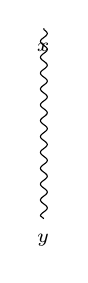
\begin{tikzpicture}[baseline={([yshift=1.4ex]current bounding box.center)}]
      \begin{feynman}[inline=(a)]
        \vertex (a);
        \vertex (b);
        \diagram {
          a -- [photon] b,
        };
        \vertex [below=0.2em of a] {\(_{x}\)};  
        \vertex [below=0.2em of b] {\(_{y}\)};  
      \end{feynman}
    \end{tikzpicture}\, .
\end{align}
The photon propagator is usually represented by a wavy line, as shown
in the second line above. 

\chapter{Divergences I - the Scalar Propagator}
\label{cha:divergences-i-scalar}

\chapter{Divergences II - the Vertex Function}
\label{cha:diverg-ii-vert}

\chapter{Renormalization}
\label{cha:renormalization}

\section{Regularization}
\label{sec:regularization}

\section{Renormalization schemes}
\label{sec:renorm-schem}



\chapter{Renormalization Group}
\label{cha:renorm-group}

\chapter{Scales - Decoupling}
\label{cha:scales-decoupling}

\printindex
\end{document}

%%% Local Variables:
%%% mode: latex
%%% TeX-master: t
%%% End:
